\documentclass[url,11pt,fleqn]{book} % Default font size and left-justified equations

%\usepackage{hyperref}
\usepackage[usenames,table,dvipsnames,svgnames]{xcolor}
\usepackage{pdfpages}
\usepackage[squaren]{SIunits}
\usepackage{acronym}
\usepackage{etoolbox}
\usepackage{multicol}
 \usepackage{vwcol}
\usepackage{placeins}
\usepackage[absolute]{textpos}
\usepackage{ulem} \normalem
\newcommand{\redcomment}[1]{{\noindent\color{red}{\it [[#1]] }}}
\newcommand{\bluecomment}[1]{{\color{blue}{\it[[#1]]}}}
\newcommand{\magentacomment}[1]{{\color{magenta}{[[ #1]]}}}
\newcommand{\greencomment}[1]{{\color{green}{[[ #1]]}}}
\newcommand{\redcommenttwo}[1]{{\color{red}{[[ #1]]}}}
\newcommand{\redtext}[1]{{\noindent\color{red}{\it #1 }}}
 \hypersetup{colorlinks=true,
            pdfstartview=FitV,
            linkcolor=Blue,
            citecolor=MediumBlue,
            urlcolor=IndianRed}
            

\textwidth 6in
\oddsidemargin 0.25 in
\textheight 8.5in
\topmargin -0.25in
%%----------------------------------------------------------------------------------------
%	VARIOUS REQUIRED PACKAGES
%----------------------------------------------------------------------------------------
\usepackage[top=3cm,bottom=3cm,left=3.2cm,right=3.2cm,headsep=10pt,letterpaper]{geometry} % Page margins
\usepackage{xcolor} % Required for specifying colors by name
\definecolor{ocre}{RGB}{52,177,201} % Define the orange color used for highlighting throughout the book

% Font Settings
\usepackage{avant} % Use the Avantgarde font for headings
%\usepackage{times} % Use the Times font for headings
\usepackage{mathptmx} % Use the Adobe Times Roman as the default text font together with math symbols from the Sym­bol, Chancery and Computer Modern fonts

\usepackage{microtype} % Slightly tweak font spacing for aesthetics
\usepackage[utf8]{inputenc} % Required for including letters with accents
\usepackage[T1]{fontenc} % Use 8-bit encoding that has 256 glyphs

% Bibliography
%\usepackage[style=alphabetic,sorting=nyt,sortcites=true,autopunct=true,babel=hyphen,hyperref=true,abbreviate=false,backref=true,backend=biber]{biblatex}
%\addbibresource{bibliography.bib} % BibTeX bibliography file
%\defbibheading{bibempty}{}


\usepackage{titlesec} % Allows customization of titles

\usepackage{graphicx} % Required for including pictures
\graphicspath{{Pictures/}{figures/cosmo/}} % Specifies the directory where pictures are stored

\usepackage{lipsum} % Inserts dummy text

\usepackage{tikz} % Required for drawing custom shapes

\usepackage[english]{babel} % English language/hyphenation

\usepackage{enumitem} % Customize lists
\setlist{nolistsep} % Reduce spacing between bullet points and numbered lists

\usepackage{booktabs} % Required for nicer horizontal rules in tables

\usepackage{eso-pic} % Required for specifying an image background in the title page

%----------------------------------------------------------------------------------------
%	MAIN TABLE OF CONTENTS
%----------------------------------------------------------------------------------------

\usepackage{titletoc} % Required for manipulating the table of contents

\contentsmargin{0cm} % Removes the default margin
% Chapter text styling
\titlecontents{chapter}[1.25cm] % Indentation
{\addvspace{15pt}\large\sffamily\bfseries} % Spacing and font options for chapters
{\color{ocre!60}\contentslabel[\Large\thecontentslabel]{1.25cm}\color{ocre}} % Chapter number
{}
{\color{ocre!60}\normalsize\sffamily\bfseries\;\titlerule*[.5pc]{.}\;\thecontentspage} % Page number
% Section text styling
\titlecontents{section}[1.25cm] % Indentation
{\addvspace{5pt}\sffamily\bfseries} % Spacing and font options for sections
{\contentslabel[\thecontentslabel]{1.25cm}} % Section number
{}
{\sffamily\hfill\color{black}\thecontentspage} % Page number
[]
% Subsection text styling
\titlecontents{subsection}[1.25cm] % Indentation
{\addvspace{1pt}\sffamily\small} % Spacing and font options for subsections
{\contentslabel[\thecontentslabel]{1.25cm}} % Subsection number
{}
{\sffamily\;\titlerule*[.5pc]{.}\;\thecontentspage} % Page number
[]

%----------------------------------------------------------------------------------------
%	MINI TABLE OF CONTENTS IN CHAPTER HEADS
%----------------------------------------------------------------------------------------

% Section text styling
\titlecontents{lsection}[0em] % Indendating
{\footnotesize\sffamily} % Font settings
{}
{}
{}

% Subsection text styling
\titlecontents{lsubsection}[.5em] % Indentation
{\normalfont\footnotesize\sffamily} % Font settings
{}
{}
{}

%----------------------------------------------------------------------------------------
%	PAGE HEADERS
%----------------------------------------------------------------------------------------

\usepackage{fancyhdr} % Required for header and footer configuration

\pagestyle{fancy}
\renewcommand{\chaptermark}[1]{\markboth{\sffamily\normalsize\bfseries\chaptername\ \thechapter.\ #1}{}} % Chapter text font settings
\renewcommand{\sectionmark}[1]{\markright{\sffamily\normalsize\thesection\hspace{5pt}#1}{}} % Section text font settings
\fancyhf{} \fancyhead[LE,RO]{\sffamily\normalsize\thepage} % Font setting for the page number in the header
\fancyhead[LO]{\rightmark} % Print the nearest section name on the left side of odd pages
\fancyhead[RE]{\leftmark} % Print the current chapter name on the right side of even pages
\renewcommand{\headrulewidth}{0.5pt} % Width of the rule under the header
\addtolength{\headheight}{2.5pt} % Increase the spacing around the header slightly
\renewcommand{\footrulewidth}{0pt} % Removes the rule in the footer
\fancypagestyle{plain}{\fancyhead{}\renewcommand{\headrulewidth}{0pt}} % Style for when a plain pagestyle is specified

% Removes the header from odd empty pages at the end of chapters
\makeatletter
\renewcommand{\cleardoublepage}{
\clearpage\ifodd\c@page\else
\hbox{}
\vspace*{\fill}
\thispagestyle{empty}
%\newpage
\fi}

%----------------------------------------------------------------------------------------
%	THEOREM STYLES
%----------------------------------------------------------------------------------------

\usepackage{amsmath,amsfonts,amssymb,amsthm} % For math equations, theorems, symbols, etc

\newcommand{\intoo}[2]{\mathopen{]}#1\,;#2\mathclose{[}}
\newcommand{\ud}{\mathop{\mathrm{{}d}}\mathopen{}}
\newcommand{\intff}[2]{\mathopen{[}#1\,;#2\mathclose{]}}
\newtheorem{notation}{Notation}[chapter]

%%%%%%%%%%%%%%%%%%%%%%%%%%%%%%%%%%%%%%%%%%%%%%%%%%%%%%%%%%%%%%%%%%%%%%%%%%%
%%%%%%%%%%%%%%%%%%%% dedicated to boxed/framed environements %%%%%%%%%%%%%%
%%%%%%%%%%%%%%%%%%%%%%%%%%%%%%%%%%%%%%%%%%%%%%%%%%%%%%%%%%%%%%%%%%%%%%%%%%%
\newtheoremstyle{ocrenumbox}% % Theorem style name
{0pt}% Space above
{0pt}% Space below
{\normalfont}% % Body font
{}% Indent amount
{\small\bf\sffamily\color{ocre}}% % Theorem head font
{\;}% Punctuation after theorem head
{0.25em}% Space after theorem head
{\small\sffamily\color{ocre}\thmname{#1}\nobreakspace\thmnumber{\@ifnotempty{#1}{}\@upn{#2}}% Theorem text (e.g. Theorem 2.1)
\thmnote{\nobreakspace\the\thm@notefont\sffamily\bfseries\color{black}---\nobreakspace#3.}} % Optional theorem note
\renewcommand{\qedsymbol}{$\blacksquare$}% Optional qed square

\newtheoremstyle{blacknumex}% Theorem style name
{5pt}% Space above
{5pt}% Space below
{\normalfont}% Body font
{} % Indent amount
{\small\bf\sffamily}% Theorem head font
{\;}% Punctuation after theorem head
{0.25em}% Space after theorem head
{\small\sffamily{\tiny\ensuremath{\blacksquare}}\nobreakspace\thmname{#1}\nobreakspace\thmnumber{\@ifnotempty{#1}{}\@upn{#2}}% Theorem text (e.g. Theorem 2.1)
\thmnote{\nobreakspace\the\thm@notefont\sffamily\bfseries---\nobreakspace#3.}}% Optional theorem note

\newtheoremstyle{blacknumbox} % Theorem style name
{0pt}% Space above
{0pt}% Space below
{\normalfont}% Body font
{}% Indent amount
{\small\bf\sffamily}% Theorem head font
{\;}% Punctuation after theorem head
{0.25em}% Space after theorem head
{\small\sffamily\thmname{#1}\nobreakspace\thmnumber{\@ifnotempty{#1}{}\@upn{#2}}% Theorem text (e.g. Theorem 2.1)
\thmnote{\nobreakspace\the\thm@notefont\sffamily\bfseries---\nobreakspace#3.}}% Optional theorem note

%%%%%%%%%%%%%%%%%%%%%%%%%%%%%%%%%%%%%%%%%%%%%%%%%%%%%%%%%%%%%%%%%%%%%%%%%%%
%%%%%%%%%%%%% dedicated to non-boxed/non-framed environements %%%%%%%%%%%%%
%%%%%%%%%%%%%%%%%%%%%%%%%%%%%%%%%%%%%%%%%%%%%%%%%%%%%%%%%%%%%%%%%%%%%%%%%%%
\newtheoremstyle{ocrenum}% % Theorem style name
{5pt}% Space above
{5pt}% Space below
{\normalfont}% % Body font
{}% Indent amount
{\small\bf\sffamily\color{ocre}}% % Theorem head font
{\;}% Punctuation after theorem head
{0.25em}% Space after theorem head
{\small\sffamily\color{ocre}\thmname{#1}\nobreakspace\thmnumber{\@ifnotempty{#1}{}\@upn{#2}}% Theorem text (e.g. Theorem 2.1)
\thmnote{\nobreakspace\the\thm@notefont\sffamily\bfseries\color{black}---\nobreakspace#3.}} % Optional theorem note
\renewcommand{\qedsymbol}{$\blacksquare$}% Optional qed square
\makeatother

% Defines the theorem text style for each type of theorem to one of the three styles above
\newcounter{dummy}
\numberwithin{dummy}{section}
\theoremstyle{ocrenumbox}
\newtheorem{theoremeT}[dummy]{Theorem}
\newtheorem{problem}{Problem}[chapter]
\newtheorem{exerciseT}{Exercise}[chapter]
\theoremstyle{blacknumex}
\newtheorem{exampleT}{Example}[chapter]
\theoremstyle{blacknumbox}
\newtheorem{vocabulary}{Vocabulary}[chapter]
\newtheorem{definitionT}{Definition}[section]
\newtheorem{corollaryT}[dummy]{Corollary}
\theoremstyle{ocrenum}
\newtheorem{proposition}[dummy]{Proposition}

%----------------------------------------------------------------------------------------
%	DEFINITION OF COLORED BOXES
%----------------------------------------------------------------------------------------

\RequirePackage[framemethod=default]{mdframed} % Required for creating the theorem, definition, exercise and corollary boxes

% Theorem box
\newmdenv[skipabove=7pt,
skipbelow=7pt,
backgroundcolor=black!5,
linecolor=ocre,
innerleftmargin=5pt,
innerrightmargin=5pt,
innertopmargin=5pt,
leftmargin=0cm,
rightmargin=0cm,
innerbottommargin=5pt]{tBox}

% Exercise box
\newmdenv[skipabove=7pt,
skipbelow=7pt,
rightline=false,
leftline=true,
topline=false,
bottomline=false,
backgroundcolor=ocre!10,
linecolor=ocre,
innerleftmargin=5pt,
innerrightmargin=5pt,
innertopmargin=5pt,
innerbottommargin=5pt,
leftmargin=0cm,
rightmargin=0cm,
linewidth=4pt]{eBox}

% Definition box
\newmdenv[skipabove=7pt,
skipbelow=7pt,
rightline=false,
leftline=true,
topline=false,
bottomline=false,
linecolor=ocre,
innerleftmargin=5pt,
innerrightmargin=5pt,
innertopmargin=0pt,
leftmargin=0cm,
rightmargin=0cm,
linewidth=4pt,
innerbottommargin=0pt]{dBox}

% Corollary box
\newmdenv[skipabove=7pt,
skipbelow=7pt,
rightline=false,
leftline=true,
topline=false,
bottomline=false,
linecolor=gray,
backgroundcolor=black!5,
innerleftmargin=5pt,
innerrightmargin=5pt,
innertopmargin=5pt,
leftmargin=0cm,
rightmargin=0cm,
linewidth=4pt,
innerbottommargin=5pt]{cBox}

% Creates an environment for each type of theorem and assigns it a theorem text style from the "Theorem Styles" section above and a colored box from above
\newenvironment{theorem}{\begin{tBox}\begin{theoremeT}}{\end{theoremeT}\end{tBox}}
\newenvironment{exercise}{\begin{eBox}\begin{exerciseT}}{\hfill{\color{ocre}\tiny\ensuremath{\blacksquare}}\end{exerciseT}\end{eBox}}
\newenvironment{definition}{\begin{dBox}\begin{definitionT}}{\end{definitionT}\end{dBox}}
\newenvironment{example}{\begin{exampleT}}{\hfill{\tiny\ensuremath{\blacksquare}}\end{exampleT}}
\newenvironment{corollary}{\begin{cBox}\begin{corollaryT}}{\end{corollaryT}\end{cBox}}

%----------------------------------------------------------------------------------------
%	REMARK ENVIRONMENT
%----------------------------------------------------------------------------------------

\newenvironment{remark}{\par\vspace{10pt}\small % Vertical white space above the remark and smaller font size
\begin{list}{}{
\leftmargin=35pt % Indentation on the left
\rightmargin=25pt}\item\ignorespaces % Indentation on the right
\makebox[-2.5pt]{\begin{tikzpicture}[overlay]
\node[draw=ocre!60,line width=1pt,circle,fill=ocre!25,font=\sffamily\bfseries,inner sep=2pt,outer sep=0pt] at (-15pt,0pt){\textcolor{ocre}{R}};\end{tikzpicture}} % Orange R in a circle
\advance\baselineskip -1pt}{\end{list}\vskip5pt} % Tighter line spacing and white space after remark

%----------------------------------------------------------------------------------------
%	SECTION NUMBERING IN THE MARGIN

%----------------------------------------------------------------------------------------\titlespacing*{<command>}{<left>}{<before-sep>}{<after-sep>}

\makeatletter
\renewcommand{\@seccntformat}[1]{\llap{\textcolor{ocre}{\csname the#1\endcsname}\hspace{1em}}}
\renewcommand{\section}{\@startsection{section}{1}{\z@}
{-2ex \@plus -1ex \@minus -.4ex}
{1ex \@plus.2ex }
{\normalfont\large\sffamily\bfseries}}
\renewcommand{\subsection}{\@startsection {subsection}{2}{\z@}
{-1ex \@plus -0.1ex \@minus -.4ex}
{0.5ex \@plus.2ex }
{\normalfont\sffamily\bfseries}}
\renewcommand{\subsubsection}{\@startsection {subsubsection}{3}{\z@}
{-1ex \@plus -0.1ex \@minus -.2ex}
{.2ex \@plus.2ex }
{\normalfont\small\sffamily\bfseries}}
\renewcommand\paragraph{\@startsection{paragraph}{4}{\z@}
{-1ex \@plus-.2ex \@minus .2ex}
{.1ex}
{\normalfont\small\sffamily\bfseries}}

%----------------------------------------------------------------------------------------
%	HYPERLINKS IN THE DOCUMENTS
%----------------------------------------------------------------------------------------

% For an unclear reason, the package should be loaded now and not later
\usepackage[colorlinks=true,citecolor=blue,linkcolor=blue]{hyperref}
%\hypersetup{hidelinks,backref=true,pagebackref=true,hyperindex=true,colorlinks=false,breaklinks=true,urlcolor= ocre,bookmarks=true,bookmarksopen=false,pdftitle={Title},pdfauthor={Author}}

%----------------------------------------------------------------------------------------
%	CHAPTER HEADINGS
%----------------------------------------------------------------------------------------

% The set-up below should be (sadly) manually adapted to the overall margin page septup controlled by the geometry package loaded in the main.tex document. It is possible to implement below the dimensions used in the goemetry package (top,bottom,left,right)... TO BE DONE

\newcommand{\thechapterimage}{}
\newcommand{\chapterimage}[1]{\renewcommand{\thechapterimage}{#1}}

% Numbered chapters with mini tableofcontents
\def\thechapter{\arabic{chapter}}
\def\@makechapterhead#1{
\thispagestyle{empty}
{\centering \normalfont\sffamily
\ifnum \c@secnumdepth >\m@ne
\if@mainmatter
\startcontents
\begin{tikzpicture}[remember picture,overlay]
\node at (current page.north west)
{\begin{tikzpicture}[remember picture,overlay]
\node[anchor=north west,inner sep=0pt] at (0,0) {\includegraphics[width=\paperwidth]{\thechapterimage}};
%%%%%%%%%%%%%%%%%%%%%%%%%%%%%%%%%%%%%%%%%%%%%%%%%%%%%%%%%%%%%%%%%%%%%%%%%%%%%%%%%%%%%
% Commenting the 3 lines below removes the small contents box in the chapter heading
%\fill[color=ocre!10!white,opacity=.6] (1cm,0) rectangle (8cm,-7cm);
%\node[anchor=north west] at (1.1cm,.35cm) {\parbox[t][8cm][t]{6.5cm}{\huge\bfseries\flushleft \printcontents{l}{1}{\setcounter{tocdepth}{2}}}};
\draw[anchor=west] (2cm,-9cm) node [rounded corners=20pt,fill=ocre!10!white,text opacity=1,draw=ocre,draw opacity=1,line width=1.5pt,fill opacity=.6,inner sep=12pt]{\huge\sffamily\bfseries\textcolor{black}{\thechapter. #1\strut\makebox[22cm]{}}};
%%%%%%%%%%%%%%%%%%%%%%%%%%%%%%%%%%%%%%%%%%%%%%%%%%%%%%%%%%%%%%%%%%%%%%%%%%%%%%%%%%%%%
\end{tikzpicture}};
\end{tikzpicture}}
\par\vspace*{230\p@}
\fi
\fi}

% Unnumbered chapters without mini tableofcontents (could be added though)
\def\@makeschapterhead#1{
\thispagestyle{empty}
{\centering \normalfont\sffamily
\ifnum \c@secnumdepth >\m@ne
\if@mainmatter
\begin{tikzpicture}[remember picture,overlay]
\node at (current page.north west)
{\begin{tikzpicture}[remember picture,overlay]
\node[anchor=north west,inner sep=0pt] at (0,0) {\includegraphics[width=\paperwidth]{\thechapterimage}};
\draw[anchor=west] (5cm,-9cm) node [rounded corners=20pt,fill=ocre!10!white,fill opacity=.6,inner sep=12pt,text opacity=1,draw=ocre,draw opacity=1,line width=1.5pt]{\huge\sffamily\bfseries\textcolor{black}{#1\strut\makebox[22cm]{}}};
\end{tikzpicture}};
\end{tikzpicture}}
\par\vspace*{230\p@}
\fi
\fi
}
\makeatother


%needed for cosmo
\usepackage{graphicx}
\graphicspath{{./figures/}}
%\usepackage{psfrag}
\usepackage{appendix}
\usepackage{latexsym,amsmath,amsfonts,amssymb,booktabs}
\usepackage[font=small]{caption}
\usepackage{slashed,upgreek,amscd,cancel,tensor,color}
\usepackage{adjustbox}
\usepackage[numbers,compress,square]{natbib}
\usepackage{epsfig,latexsym}
%\usepackage[pdfencoding=auto]{hyperref}
\usepackage{url}
\numberwithin{equation}{section}% numera le equazioni seconde le sezioni , e.g. 1.15 invece che consecutivamente; anche le appendici, eq. (A.1) etc. Richiede amsmath
\usepackage{doi}
\usepackage{subcaption}
\usepackage{mathtools}
\usepackage{upgreek}
\usepackage{stfloats}
\usepackage{afterpage}
\usepackage{multirow}

%\newcommand{\mnras}{MNRAS}
%\newcommand{\aap}{A\&A}
%\newcommand{\nat}{Nature}
%\newcommand{\araa}{Annual Review of Astronomy and Astrophysics}
%\newcommand{\araa}{ARAA}
%\newcommand{\apj}{ApJ}
%\newcommand{\apjl}{ApJL}
%\newcommand{\aj}{AJ}
%\newcommand{\prd}{Physical Reviews D}
\newcommand{\aapr}{Astronomy and Astrophysics Reviews}

\definecolor{antiquewhite}{rgb}{0.98, 0.92, 0.84}
\definecolor{aliceblue}{rgb}{0.94, 0.97, 1.0}
\definecolor{blanchedalmond}{rgb}{1.0, 0.92, 0.8}
\definecolor{beaublue}{rgb}{0.74, 0.83, 0.9}
\definecolor{beaubluedark}{rgb}{0.79, 0.85, 0.95}
\definecolor{amber(sae/ece)}{rgb}{1.0, 0.49, 0.0}
\definecolor{airforceblue}{rgb}{0.36, 0.54, 0.66}
\definecolor{aliceblue}{rgb}{0.94, 0.97, 1.0}
\definecolor{alizarin}{rgb}{0.82, 0.1, 0.26}
\definecolor{almond}{rgb}{0.94, 0.87, 0.8}
\definecolor{amaranth}{rgb}{0.9, 0.17, 0.31}
\definecolor{amber}{rgb}{1.0, 0.75, 0.0}
\definecolor{amber(sae/ece)}{rgb}{1.0, 0.49, 0.0}
\definecolor{americanrose}{rgb}{1.0, 0.01, 0.24}
\definecolor{amethyst}{rgb}{0.6, 0.4, 0.8}
\definecolor{anti-flashwhite}{rgb}{0.95, 0.95, 0.96}
\definecolor{antiquebrass}{rgb}{0.8, 0.58, 0.46}
\definecolor{antiquefuchsia}{rgb}{0.57, 0.36, 0.51}
\definecolor{antiquewhite}{rgb}{0.98, 0.92, 0.84}
\definecolor{ao}{rgb}{0.0, 0.0, 1.0}
\definecolor{ao(english)}{rgb}{0.0, 0.5, 0.0}
\definecolor{applegreen}{rgb}{0.55, 0.71, 0.0}
\definecolor{apricot}{rgb}{0.98, 0.81, 0.69}
\definecolor{aqua}{rgb}{0.0, 1.0, 1.0}
\definecolor{aquamarine}{rgb}{0.5, 1.0, 0.83}
\definecolor{beaver}{rgb}{0.62, 0.51, 0.44}
\definecolor{blizzardblue}{rgb}{0.67, 0.9, 0.93}
\definecolor{azure}{rgb}{0.0, 0.5, 1.0}

\usepackage{pdfpages}
\usepackage[squaren]{SIunits}
\usepackage{acronym}
\usepackage{etoolbox}
\usepackage{multicol}
 \usepackage{vwcol}
\usepackage{placeins}
\usepackage[absolute]{textpos}
\usepackage{ulem} \normalem
\usepackage{tcolorbox}
\newcommand{\redcomment}[1]{{\noindent\color{red}{\it [[#1]] }}}
\newcommand{\bluecomment}[1]{{\color{blue}{\it[[#1]]}}}
\newcommand{\magentacomment}[1]{{\color{magenta}{[[ #1]]}}}
\newcommand{\greencomment}[1]{{\color{green}{[[ #1]]}}}
\newcommand{\redtext}[1]{{\noindent\color{red}{\it #1 }}}


\begin{document}
%\linenumbers
%\title{GWIC 3G R\&D Subcommittee Report }
%\author{
v.d. Brand, Jo, \texttt{jo@nikhef.nl} 
\and
McClelland, David, \texttt{david.mcclelland@anu.edu.au}
\and
L\"uck, Harald,   \texttt{harald.lueck@aei.mpg.de} 
%Inst. f. Gravitationsphysik, Leibniz Universitaet Hannover and Max-Planck Institut f. Gravitationsphysik, Hannover, Germany; 
\and
Adhikari, Rana, \texttt{rana@caltech.edu}
\and
Billingsley, Garilynn, \texttt{billingsley\_g@ligo.caltech.edu}
\and
Cagnoli, Gianpietro, \texttt{cagnoli@lma.in2p3.fr}
\and
Evans, Matthew, \texttt{mevans@ligo.mit.edu}
\and
Fejer, Martin, \texttt{fejer@stanford.edu}
\and
Freise, Andreas, \texttt{adf@star.sr.bham.ac.uk}
\and
Fulda, Paul, \texttt{pfulda@phys.ufl.edu}
\and
Gemme, Gianlucca, \texttt{gianluca.gemme@ge.infn.it}
\and
Genin, Eric, \texttt{eric.genin@ego-gw.it}
\and
Gonzalez, Gabriela, \texttt{gonzalez@lsu.edu}
\and
Harms, Jan, \texttt{jan.harms@gssi.it}
\and
Hild, Stefan, \texttt{stefan.hild@glasgow.ac.uk}
\and
Losurdo, Giovanni, \texttt{giovanni.losurdo@pi.infn.it}
\and
Lough, James, \texttt{James.Lough@aei.mpg.de}
\and
Martin, Ian, \texttt{iain.martin@glasgow.ac.uk}
\and
Massaki, Ando,  \texttt{ando@phys.s.u-tokyo.ac.jp}
\and
Prabhakar, Anil, \texttt{anilpr@ee.iitm.ac.in}
\and
Reid, Stuart, \texttt{Stuart.Reid@uws.ac.uk}
\and
Ricci, Fulvio, \texttt{fulvio.ricci@roma1.infn.it}
\and
Robertson, Norna, \texttt{nroberts@ligo.caltech.edu}
\and
Willke, Benno, \texttt{Benno.willke@aei.mpg.de}
\and
Yamamoto, Kazuhiro \texttt{yamak@icrr.u-tokyo.ac.jp}
}
%\date{\today}
%\maketitle
%\tableofcontents
%\newpage
%\chapter{Research and development for a 3G GW observatory network}
\label{chap:RaD}
\chapterimage{Figures/ArtisticView2.jpg} % Chapter heading image
%Einstein Telescope artits impression copyright Nikhef
%\section{Introduction}
\chapter{Introduction}
\label{sec:Intro}

In this part of the report we review the Research and Development needed to construct and operate detectors of "third generation" or "3G" sensitivity. As with the first set of long baseline facilities (LIGO, Virgo, KAGRA)~\cite{AdvancedVirgo2015,AdvancedLIGO2015,KAGRA2013}, the new 3G facilities will be designed and built to house a number of generations of detectors with increasing sensitivity as technology evolves and new ideas emerge. Section 3.2 will cover the R\&D needed to build such large, long-life-time facilities in a cost efficient way. The remainder of this part will focus on the R\&D required to deliver the first detectors operational in these 3G facilities. Currently, there are two main concepts for these detectors, the Einstein Telescope (ET)~\cite{ET2011} and Cosmic Explorer (CE)~\cite{CosmicExplorer2017}.

\begin{figure}[ht]
\centering
%\begin{multicols}{2}
% \begin{vwcol}[widths={1.06,0.84},justify=flush,rule=0pt] 
%\centering
%\vspace{-0.15cm}
%\includegraphics*[width= 1.0 \columnwidth]{Figures/noises_percentiles.pdf}
%\columnbreak
\includegraphics*[width= 0.8\textwidth]{Figures/noises_percentiles.pdf}
\caption{Currently, there are two main designs proposed for 3G: the Einstein telescope (ET) \cite{ET2011} with the goal sensitivity shown in green and Cosmic Explorer (CE) \cite{CosmicExplorer2017} with goal sensitivity shown in pink.  Also shown are the aLIGO design sensitivity (blue curve) and the goal sensitivity for LIGO Voyager (orange curve). The shades of the curves represent sensitivity to sources with differently distributed locations.}
\label{fig:3GSens}
%\end{vwcol} 
%\end{multicols}
\end{figure}

The 3G instruments will be 10 to 20 times more sensitive than 2G in the frequency band above  100\,Hz.  This rises to up to a factor of 100 around 20\,Hz and factors of thousands to millions below 10\,Hz. 
% Despite their differences in sensitivity, 
The 'enabling technologies' -- the main pillars on which the predictions of sensitivity are based --  are similar for ET and CE. They aim to mitigate 'fundamental noise sources' affecting the instruments, in particular: \textbf{Quantum noise} is modified by high laser power, quantum squeezing and interferometer topology; \textbf{Thermal noise} in mirror substrates, coatings and suspensions is modified by temperature and material properties (and their behaviour as a function of temperature); And \textbf{Newtonian noise} is modified by the location of the sites and subtraction schemes. 
% quantum noise, thermal (Brownian) noise and Newtonian noise. 
%Seismic noise and residual gas noise had been listed as fundamental noises, but as they are treatable by more expensive technology we do not list them as fundamental here.
   
These considerations are not independent of each other. Using low temperatures to reduce Brownian noise requires moving away from the fused silica optics used in Advanced LIGO and Advanced Virgo. Sapphire and Silicon are promising low temperature materials. Silicon would require changing the operating wavelength to 1.5 -- 2\,\micro m, necessitating the development of a new suite of light sources, optical components and detectors.  Considering material properties as a function of temperature and wavelength along with the ability to handle high optical power whilst noiselessly removing heat from the core optics leads to four candidate operating temperatures:  room temperature and cryogenic temperatures 123\,K, 15\,K and below 5\,K.  

Sections \ref{sec:Fac_Inf} to \ref{sec:Newtonian_Noise} consider the state of the art in enabling technologies, the R\&D needed in each area, the level of resources needed (broadly bracketed as high, medium, low),
% \magentacomment{This is not implemented in the report} 
and how the R\&D should be organized and coordinated, in order to deliver fully tested subsystems for timely installation in new 3G facilities. Prototyping will require new test facilities and/or using existing long baseline facilities.
In addition to fundamental noises, a myriad of technical noise sources and control issues can limit interferometer performance: parametric instabilities, scattered light, and noise originating from auxiliary optics and control systems.  The current state of the art in these areas, R\&D needed, and coordination for 3G are reviewed in sections \ref{sec:Aux-optics} and \ref{sec:Sim_Controls}. 

Two detector epochs are envisioned 
% post advanced detector baseline sensitivities 
to follow the advanced detectors over the next 25\,years: upgrades in existing facilities; % operating at 1\,$\mu m$ wavelength; 
and new detectors in new, longer baseline, third generation (3G) facilities. This strategy will be modified according to signals observed, technology readiness and funds available.
%The 3G facility infrastructure can to some extent be decoupled from the initial 3G instruments. 
The 3G facilities are being designed with lifetimes up to 50 years and to be suitable for both initial instruments with sensitivities 10 times that of the advanced detectors and upgrades that may achieve another factor of 10. There are currently two designs for such facilities:  The Einstein Telescope (ET) is envisaged as an underground facility capable of housing three pairs of detectors in a nested triangular vacuum envelope with three 10\,km sides. Cosmic Explorer is proposed to be a single L-shaped facility with two 40\,km arms. The most effective 3G network would incorporate a pair of widely separated Cosmic Explorers working in unison with the Einstein Telescope~\cite{Hall:2019xmm}.

\begin{tcolorbox}[standard jigsaw,colback=amber!10!white,colframe=red!70!black,coltext=black, title=The Einstein gravitational--wave Telescope (ET)] ET~\cite{ET2011} is the European concept for a third generation gravitational-wave \emph{observatory}. To reduce the effects of seismic motion, the ET concept calls for the site to be located at a depth of about 100\,m to 200\,m below ground. In its final configuration it shall be arranged as an equilateral triangle of three interlaced detectors, each consisting of two interferometers. The configuration of each detector dedicates one interferometer (ET-LF) to detecting the \textbf{L}ow \textbf{F}requency components of the gravitational-wave signal (2--40\,Hz), while the other one (ET-HF) is dedicated to the \textbf{H}igh \textbf{F}requency components. Each interferometer will have a dual-recycled Michelson layout with Fabry-Perot arm cavities of about 10\,km arm length. In ET-LF, which operates at cryogenic temperature, thermal, seismic, gravity gradient and radiation pressure noise sources are particularly suppressed; in ET-HF, sensitivity at high frequencies is improved by high laser light power circulating in the Fabry--Perot cavities and the use of frequency-dependent squeezed light technologies.
\end{tcolorbox}

\begin{tcolorbox}[standard jigsaw,colframe=azure!70!black,colback=azure!20!white,opacityback=0.6,coltext=black, title= LIGO Voyager]
LIGO Voyager~\cite{Voyager:Inst,VoyagerDCC2018} is the tentative concept for a new detector in the current LIGO observatory facilities designed to maximize the observational reach of the LIGO infrastructure and demonstrate the key technologies to be used for 3G observatories in new infrastructures.
Voyager would use heavy (ca.\,200\,kg) cryogenic mirrors with improved coatings and upgraded suspensions made of ultra-pure silicon at a temperature of 123\,K in the existing LIGO vacuum envelope and a laser wavelength of $\sim1.5\,-\,2\,\mu m$. 
A further factor of 3 increase in BNS range (to 1100\,Mpc) is envisioned along with a reduction of the low frequency cutoff down to 10 Hz. In the context of this report we use the term \emph{Voyager Technology} for this type of technology irrespective of plans to implement it in any existing or future infrastructure.
\end{tcolorbox}

\begin{tcolorbox}[standard jigsaw,colframe=antiquefuchsia!80!black,colback=antiquefuchsia!20!white,opacityback=0.6,coltext=black, title=Cosmic Explorer (CE)] 
CE~\cite{CosmicExplorer2017} is a US concept envisioning an L-shaped above-ground observatory with 40\,km arm-length, operating a dual recycled Michelson interferometer with Fabry--Perot arm cavities. 

CE~\cite{CosmicExplorer2017} is a US concept that envisions 40\,km long arms and new technologies to achieve a factor of 10 or more strain sensitivity improvement over the current generation of gravitational-wave detectors. As with LIGO, it will employ a dual recycled Michelson interferometer with Fabry--Perot arm cavities and be implemented in stages. Its initial phase, called CE1, will employ scaled-up \emph{aLIGO technology} and frequency-dependent squeezing. 
% Frequency-dependent squeezing will improve the quantum limited sensitivity by a factor of three. 
A major upgrade, CE2, will exploit the full potential of the new facility by using \emph{Voyager technology} such as silicon test masses and amorphous silicon coatings operating at 123\,K, with $1.5$ or $2\,\mu m$ laser light and 3\,MW of optical power in its arm cavities.
\end{tcolorbox}

Planning for the 3G detectors began more than 20 years before they are envisioned to operate. This was based on experience with past and current detectors, for which there was a lead time of 15 years or more from conception to operation. Assuming a 2035 start date for initial 3G operations preceded by five years of construction and five years of commissioning, it is likely that only technologies with mature R\&D in 2025 will feed into final design and engineering for the initial 3G detectors. In this document we assess the state of the enabling subsystem R\&D toward readiness in 2025 while also looking ahead to the R\&D that will continue as a necessary preparation for subsequent 3G upgrades. Prototyping such technology may include testing performance and science capability in an existing 2G facility. The term "Voyager" is used to describe a detector in a 2G facility that would prototype CE phase 2 technology whilst significantly improving detection range. 

\begin{table}[h]
\centering
\begin{tabular}{|l|l|l|p{1.6cm}|l|l|l|l|}
\hline
 % \multicolumn{8}{|c|}{Current and Future Interferometers}\\ 
 %\hline
 &aLIGO / AdV &A+/V+ &KAGRA &CE 1 &CE 2 &ET-LF &ET-HF\\
\hline
Arm Length [km] & 4 / 3 &4& 3& 40& 40& 10 &10\\
\hline
Mirror Mass [kg]& 40 / 42& 40& 23& 320& 320& 211& 200\\
\hline
Mirror Material& silica& silica& sapphire& silica& silicon& silicon& silica\\
\hline
Mirror Temp [K]& 295& 295& 20& 295& 123& 10& 290\\
\hline
Suspension Fiber& 0.6m/0.7m& 0.6m& 0.35m& 1.2m& 1.2m& 2m& 0.6m\\
& SiO2& SiO2&Al2O3&SiO2&Si&Si&SiO2\\
\hline
Fiber Type& Fiber& Fiber& Fiber& Fiber& Ribbon& Fiber& Fiber\\
\hline
Input Power [W]& 125& 125& 70& 150& 220& 3& 500\\
\hline
Arm Power [kW]& 710 / 700& 750& 350& 1400& 2000& 18& 3000\\
\hline
Wavelength [nm]& 1064& 1064& 1064& 1064& 1550& 1550& 1064\\
\hline
NN Suppression& 1& 1& 1& 10& 10& 1& 1\\
\hline
Beam Size [cm]& (5.5/6.2) / 6& 5.5/6.2& 3.5/3.5& 12/12& 14/14& 9/9& 12/12\\
\hline
SQZ Factor [dB]& 0& 6& foreseen& 10& 10& 10& 10\\
\hline
F. C. Length [m]& none& 300& unknown& 4000& 4000& 10000& 500\\
\hline
\end{tabular}
\caption[FutIfos]{Interferometric parameters for the current Advanced detectors, the upgrades thereof (LIGO A+ and advanced {\bf V}irgo +), the two phases of Cosmic Explorer (CE1 and CE2) and the two interferometer types of the Einstein Telescope.}
\label{FutIfos}
\end{table}
\magentacomment{hal: please check values}
\clearpage
\chapterimage{Figures/Virgotube.jpg} % Chapter heading image
% Virgo beam tube copyright Virgo/EGO
\chapter{Facilities and Infrastructures}
%\section{Facilities and Infrastructures}
\label{sec:Fac_Inf}
test
The characteristics of the site location and of the infrastructure directly impacts the final sensitivity and achievable observation time of the detector. Ground vibrations not only affect the sensitivity directly, through seismic and Newtonian noise couplings, but 
% may also do it indirectly 
also indirectly though additional scattered light noise and 
%making the overall control more difficult).
complicating interferometer control.
Therefore, local noise (of natural or anthropic origin) is one of the key parameters for the evaluation of a candidate site.  Construction of underground detectors (such as ET) must consider the nature of the rock, homogeneity over the arm lengths, abundance of water, long term geological stability both as cost drivers and overall site quietness. 
%are aspects which can impact the infrastructure cost and stability. These aspects are particularly relevant for underground infrastructure such as the one planned for hosting the ET detector.

%Optimizing the site facility and infrastructure's influence on  detector performance is only one aspect of the R\&D work required.  
In addition to the of site, the design of the 
Civil facilities and vacuum systems are likely to dominate the total project construction costs.  Every effort to minimize costs, cost %uncertainties, 
contingencies, and other collateral impacts on society in these domains will reap rewards,  potentially pivotal, in approval and sponsorship. 

\section{High Level Design Considerations}
\label{Req:Fac_Inf}
%Quantitative requirements and figures-of-merit for site selection and infrastructure implementation still need to be worked out, but a 
A high-level list of considerations includes aspects such as:
\begin{itemize}
\item intensity of seismic noise (on surface and underground)
\item surface meteorological conditions (wind, rain)
\item anthropogenic noise (population density, presence of industrial activity)
\item geological stability
\item earthquake history
\item type of the underground rock (for tunnel construction feasibility and cost) 
\item underground water abundance
\item orography
% Dave R adds:
\item regional and national permitting and environmental clearances
\item site levelness (for above ground detectors)
\item proximity to urban centers (for live-ability)
\end{itemize}
\newpage
For underground detectors, the design of the %caverns
experimental halls %hosting the corners of the detector 
require a special attention. They have to be large enough %in order to ease 
to facility assembly and maintenance of detector components %equipment and operation  and, above all, not to prevent 
to accommodate future %evolution of the detector. 
upgrades. On the other hand, the larger the volume the larger the cost and the engineering challenge. Cavern volume and shape also contribute to the level of atmospheric Newtonian noise (Section \ref{sec:Newtonian_Noise}) which might limit the sensitivity.

For surface %concepts, 
detectors such as Cosmic Explorer, many of these same criteria are in effect; indeed, for a putative 40km laser-straight arm, the Earth’s sagitta is of order 30m, somewhat blurring the concept of “surface” construction. This approach does, however, promote surface topography and surface geology in their priorities as site criteria. The direct effect of wind on above-ground structures also joins its indirect influences on seismicity and gravitational gradients. Effects on the artificial and natural environment, flora and fauna are also concerns, and must be factored differently into site selection, project approval, and design. 

Advances in tunnel boring machines and in surface road and pipeline excavation have been seen to drastically reduce the cost per kilometer of public works structures over recent decades, e.g.,~\cite{BoringCompany}. Directed research into applying these modern methods to reduce the cost and collateral impact of projects such as ET and CE should be explored as a high priority. 
Attention must be also paid to the legal aspects specific to each candidate countries, which could impact the timing of the infrastructure realization. 

\subsection{3G initial/future}\magentacomment{hal: derive required action items (JRS: Subscale demos, current gen equipment noise surveys)}
\greencomment{Dave: I had to read this section before I understood what it was about.  It needs a few introductory sentences to make it clear  to the reader what this section is consider.}

I think this is better located at the end of the facilities section.  Also, if we become pushed to make cuts to save space; I think this section could be cut. 
As far as the civil infrastructure is concerned we cannot think of a phased approach. In the ET case the excavation of the underground infrastructure and the realization of the ground auxiliary works must be done once for all. It is a matter of realizing an expensive infrastructure, which must be working for decades and must therefore be stable  and capable of hosting the evolution of the detector.

With respect to vacuum systems, 1G/2G experience suggests different approaches. LIGO elected to bake out and qualify its beam tubes for asymptotic "2G" service (about $10^{-9}$ Torr $\rm H_2$ and $10^{-11} $ Torr $\rm H_2O$) immediately at inception, but invested in no durable means to repeat this in future; Virgo chose to provide a permanent bake capacity, but to delay the expense of exercising the bakeout until it is required for observing sensitivity. In the construction phase, the  KAGRA interferometer devoted  a special care to smooth   the inner surface of the tube via electropolishing, a costly approach that could fulfill  residual pressure requirements without baking the vacuum system  after assembly.  Each was a valid approach in its specific Project context; whether phased performance criteria (and some opportunity for cost savings) makes sense for 3G beam tubes will depend on many factors, including future operations funding and the future global observing plan.  


\section{Impact/relation to 2G and upgrades}

There is still room to\textbf{improve the sensitivity of the 2G detectors through incremental upgrades}. However, in the next years we expect to reach the "\textbf{infrastructure limit}". In other words, the level of environmental noise as well as the detector lengths and even the space available in the buildings will make it hardly possible or to expensive to improve further. The ET underground infrastructure is conceived to overcome such limits. \greencomment{Dave: I realize this may be a controversial opinion not shared by all, but an infrastructure that is limited to $L=10 km$ will require all the improvements to come from making better measurements of $Delta_L$.  That seems a harder road to me...} However, it is crucial to understand those limits and be sure that all the lessons have been learned. For instance, the quietness of an underground location can be spoiled by machine-induced noise. It is therefore very important to review the machine-induced noise in the current infrastructures and engineer the new site in order to minimize such disturbances. A joint effort based on the LIGO, Virgo and particularly KAGRA experience on this topic would be beneficial. 

In current practice, incremental upgrades of existing detectors like LIGO, GEO600  and Virgo have been an effective way to prove new technologies in context, at full sensitivity, while directly expanding the observing horizon. Enhanced LIGO, Advanced LIGO, Advanced Virgo, Virgo+ and A+ are examples of this effective combination of R\&D and practical deployment ``on the fly''  for improved observations.  

The incremental upgrade approach has limits, however.  One is the constraint to maintain compatibility with legacy systems and infrastructure; new topologies, footprints, and even wavelengths may be effectively off the table. Less obvious, but potentially more serious, is the growing imperative to minimize interruptions to observing. Upgrades require downtime.  The explosive discoveries of the last three years, particularly the multimessenger astronomy revolution triggered by GW170817,  have raised global desire to keep observing with existing 2G and 2G+ instruments. 

As a result, an increasing portion of 3G technology demonstration must rely on offline engineering development in subscale demonstrations, reprising the  development environment of initial LIGO and Virgo, before any large-scale testbed existed. 

\section{3G vacuum systems}
Vacuum systems for planned 3G detectors are likely to be the largest ultra-high vacuum systems built to date and will account for a significant part of the cost of building the observatories. Substantial innovation and research went into designing and building the LIGO, Virgo, GEO600 and KAGRA vacuum systems within economic constraints; the more stringent technical requirements and much greater size required for 3G vacuum envelopes threaten to render them infeasible without still further innovation. Many avenues for technical research have been proposed,  centered on themes of either improving an interferometer’s immunity to residual gas, or reducing the cost of suitable installations. Some questions that merit closer investigations include:

\begin{itemize}
\item  Are there economies in using materials other than stainless steel as the envelope material? What is really known about the vacuum properties of the inexpensive tubing (e.g., cold rolled steel) used for petroleum and gas transport? What are the vacuum experience and costs associated with aluminum alloys and plastics?

\item Are nested (e.g., differentially pumped) vacuum systems practical and would they offer cost advantages? For example, can an outer pressure vessel of inexpensive structural material protect a thin liner of UHV-compatible, bakeable material?

\item Can civil construction mass-production techniques, such as extrusion and spiral tube milling, be adapted to future UHV construction?

\item Are there newer mass production surface treatment and cleaning techniques that can be applied reduce outgassing? Is heating the best degassing method, or can UV or plasma excitation be cost-competitive at scale?

\item Are there ways to simultaneously meet surface outgassing and possibly distributed pumping together with other physical requirements of the system, such as (e.g. for gravitational wave applications) stray light attenuation, vibration damping and particulate mitigation?

\item Can optical pressure gauging and leak detection offer practical advantages for system construction, commissioning and maintenance?

\item What are the prospects for new getter materials and surface treatments in maintaining UHV conditions for very large systems with modest gas loads?

\item Are there new ideas for reliable, affordable large-aperture gate valves to isolate from atmospheric pressure during construction and service, and to isolate volumes with different requirements?

\item What are effective methods or surface treatments to minimize moisture adsorption during vented system service access? Are there efficient means to accelerate desorption during pumpdown and recovery?

\end{itemize}



\section{Pathways and required facilities}
\section{Type of collaboration required:  small/large}
collaboration with high energy particle physics community (know-how in building large vacuum systems from accelerator facilities)

\section{Suggested mechanisms}
\magentacomment{Josh: Would be good to get report, or whatever we can from the LLO vacuum workshop.}
\clearpage
\chapterimage{Figures/CoreOptics.jpg} % Chapter heading image
% aLIGO optics copyright LSC/LIGO
%\section{Introduction}
\chapter{Core Optics}
%\section{Core Optics}
\label{sec:Core_optics}
%\section{Background}

% For 3G detectors there is a strong interdependence among the core optic substrate material, operating temperature, and laser wavelength.

The substrate materials that will be used for core optics in the 3G detectors are interdependent on the operating temperatures of those detectors (Section~\ref{sec:Cryogenics}) and the laser wavelengths to be used (Section~\ref{sec:Light_sources}). 
Thermal noise plays a strongly limiting role in all current gravitational-wave detectors. At room temperature, fused silica, which is used in LIGO and Virgo, is an excellent substrate material due to its very low thermoelastic effect and ultra low optical~\cite{GEO_Absorption} and mechanical losses~\cite{Ageev_2004}. Many planned detectors
% Thermal noise will limit the sensitivity of all current gravitational wave detectors. Many planned detectors and upgrades will use cryogenic cooling of the mirrors to reduce thermal noise -- 
including KAGRA~\cite{KAGRA2013}, LIGO Voyager~\cite{VoyagerDCC2018}, the Einstein Telescope low-frequency detector (ET-LF)~\cite{ET2011} and the upgrade to Cosmic Explorer (CE2)~\cite{CosmicExplorer2017} will operate at cryogenic temperatures to reduce thermal noise. 
% At cryogenic temperatures, fused silica suffers from a broad and high peak in mechanical loss~\cite{Travasso_2007}, and cannot be used. 
Fused silica is not a suitable mirror substrate material at cryogenic temperatures due to strongly increased low-temperature mechanical loss~\cite{Travasso_2007}.
In general, crystalline materials have much less Brownian noise at cryogenic temperatures than at room temperature due to their ordered lattice structure.
% a very large peak in mechanical loss centred on $\sim$40\,K, which would result in a significant increase in thermal noise on cooling a silica mirror to temperatures below 100 K.
Sapphire, which is used in KAGRA at 20\,K~\cite{Hirose_2014a}, and silicon, which is planned for use in Voyager, ET, and CE2, have especially promising performance including low mechanical loss at cryogenic temperatures. 
% for the key considerations of cryogenic gravitational-wave detectors.
% The two materials that are most commonly considered for use at cryogenic temperatures are sapphire, which is used in Kagra at 20\,K~\cite{Hirose_2014a}, and silicon, which is planned for use in Voyager, ET, and CE2. 
% Both materials can have low mechanical loss at cryogenic temperatures, essential for keeping the substrate contribution to thermal noise low. 

%In addition to low thermal noise, 
3G detector core optics must also meet a number of other challenging requirements. Uniform and pure masses of several hundred kg (see Table~\ref{Tab:FutIfos}), significantly more than currently in use, are required to reduce radiation pressure noise and accommodate larger diameter laser beams in order to better reduce (through averaging, see figure~\ref{fig:Thermal_Noise}) thermal noise. Optical absorption and scatter must both be low. The ET Design Study~\cite{ET2011} specifies a scatter loss of 37.5\,ppm per mirror surface. We note that there is excess scatter loss in the arm cavities of the advanced detectors, and further understanding of this will be important to reach the 3G scatter requirements. Finally, requirements for test mass cooling for Voyager and ET-LF lead to requirements for the optical absorption of the input test mass substrates to be less than $\sim$10\,ppm/cm.

The major open questions for core optics materials that must be addressed by 3G R\&D are described below with a focus on fused silica, silicon and sapphire. More details are given in Appendix~\ref{sec:Appendix_Core_optics}.


%\magentacomment{hal: Is this paragraph required or does a link to suspensions and cryogenics suffice?} Extraction of the laser power absorbed in the mirrors (and their coatings) will be an important consideration, impacting on the operating temperature of the mirror. For mirrors at 123 K, as proposed for LIGO Voyager, significant cooling power is provided by thermal radiation. Mirrors operating at lower temperatures will need to rely largely on conduction through the suspension fibres for heat extraction. It should be noted that heat extraction at 10 K has significant implications for the design of suspension fibres, and thus for suspension thermal noise, with one study suggesting silicon fibre diameters approaching 4mm may be required.

%The optical absorption requirement is set by a combination of the desired operating temperature, the potential for heat extraction from the cold mirror and the desired laser power in the interferometer. For LIGO Voyager, with  3\,kW power on the central interferometer and assuming a maximum radiative cooling power of 10\,W, the allowable absorption in the ITM is less than 15\,ppm/cm.  For ET-LF, with $\sim$850\,W %18\,W 
%of central interferometer power and assuming a cooling power of 100\,mW via conduction through the suspension fibres, a similar absorption requirement of less than 11\,ppm/cm is found. \magentacomment{hal: pretty sure the numbers were wrong. check powers stated here. It seems that the PRC power and the power absorbed in the ITMs has been disregarded (forgotten???) in the ET DS. 11ppm/cm in the ET-LF ITMS leads to 17mW absorbed power, similar to what was assumed for intracavity surface absorption.}


%\section{Candidate materials for low noise substrates}
% \magentacomment{This paragraph and the first one above are so similar...I'll merge them later}
 
% The main challenge is the production of homogeneous large volume crystalline substrates with low enough defects and optical absorption.

\section{Fused Silica} 
For fused silica, homogeneity of the refractive index is an important consideration. For the substrates of the cavity mirrors, excellent homogeneity is only important in the two dimensions perpendicular to the beam axis. This can be achieved even for large volumes (corresponding to a total mass of several hundred kilograms). However, the beam splitter requires a very high homogeneity in all three dimensions and this can currently only be guaranteed by the manufacturers for masses up to 40 kg (diameter 55 cm, thickness 7 cm). The company Heraeus has planned some tests to push this limit to about 100 kg. Whether such large beam splitters are required depends on the optical layout of the detector and is under investigation.

\section{Silicon}
Silicon has a low mechanical loss at cryogenic temperatures (similar below 10 K to fused silica's at room temperature).
% , resulting in low substrate thermal noise. 
In addition, the thermal expansion coefficient of silicon is zero at $\sim$123\,K and 18\,K which allows, with temperature control, the suppression of substrate thermoelastic noise and thermal expansion effects due to absorbed laser power.

Silicon is opaque at the currently used wavelength of 1064\,nm. Initially, the telecommunications wavelength of 1550\,nm was proposed for use with silicon mirrors, due to wide availability of high-powered lasers and optical components. More recently, there has been growing interest in using a wavelength close to 2000\,nm. A major driver towards 2000\,nm is the development of amorphous silicon as a possible low thermal noise cryogenic coating material. Amorphous silicon exhibits significantly lower absorption (a factor of $\sim$7) at 2000\,nm than at 1550\,nm. It seems likely, therefore, that the choice of mirror coatings will be a major factor in the choice of wavelength for future detectors. 

Sufficiently low optical absorption can be obtained from silicon refined with the Float Zone technique, however, the maximum size for this method is $\sim$200\,mm. This is too small for the requirements of future detectors (e.g. ET-LF requires 450\,mm diameter, 550\,mm thick optics and CE2 upto 700\,mm diameter optics). While larger diameter silicon pieces can be produced using the Czochralski method, the optical absorption of this type of silicon is too high, due to impurities related to the production method. A magnetic Czochralski process (MCz) exists, in which a magnetic field is used to reduce the impurity concentration in the centre of the ingot. This process can produce diameters of up to 450 mm, and a production line for manufacturing silicon of this diameter does exist at the company Shin Etsu, but is currently not operational. Initial studies of the optical absorption have shown low values at room temperature of $\sim$3\,ppm/cm at 1550\,nm and $\sim$5\,ppm/cm at 2000\,nm. The measurements showed an increase towards lower temperatures, reaching approximately 10\,ppm/cm at 50\,K, meeting the requirement for cryogenic silicon mirrors of the ET design study. However, initial studies indicate that the absorption of this material can vary significantly, both along the radius and along the length of an ingot, and more studies of the homogeneity of the absorption and its dependence on the thermal history of the sample are required. 

There is evidence that polishing silicon surfaces can increase their optical absorption. The presence of surface absorption was confirmed in a study in the IGR in Glasgow \cite{SiliconSurfaceAbsorpBell2017} and it was shown that a proprietary polishing process can be used which does not produce this effect. While this has been consistently demonstrated, further work is required to test whether a silicon surface can be polished to the specifications required for a GW detector without resulting in surface absorption.

Non-linear absorption in silicon is not expected to set a major limit to performance, contributing <\,0.5\,ppm/cm absorption for a wavelength of 2\,$\mu$m at the light intensity assumed for inside the LIGO Voyager ITM. At the significantly lower intensity within an ET-LF ITM, these effects are even less significant. Two-photon absorption generates free carriers in silicon: the absorption due to these free carriers depends crucially on the carrier life time. Experiments to measure this for magnetic Czochralski silicon are underway in a collaboration between Stanford and Glasgow.

% \greencomment{Dave: I like including absorption mechanisms in this section.  But you don't talk about free carrier absorption, impurity absorption, etc... Presumably there are the main sources of absorption?  }

It will be important to test the optical scattering from MCz silicon, particularly as the MCz growth process is known to produce a high void content in the material. Work on this is underway at Glasgow and at Caltech. Initial scattering estimates at Glasgow~\cite{SiliconScatter2017} suggest that the scattering is higher than in fused silica, but is likely to be within the required limits.

\section{Sapphire}
Sapphire is transparent at 1064\,nm and hence does not require changing the currently used laser wavelength. It has low mechanical loss at room temperature~\cite{Rowan_2000a} and even lower loss at cryogenic temperatures\cite{uchiyama1999mechanical}. 
% On mirror-size samples measurements are affected by the suspension systems used. 
Sapphire's elastic constants are about 3 times higher than silicon's, helping to reduce thermal noise (\ref{fig:Thermal_Noise}). The high Young's modulus of elasticity has two additional advantages: fewer parametric instabilities and a higher internal resonance frequencies. The thermal conductivity of sapphire increases with decreasing temperature and reaches a peak of several $10^3$\,W/(m \,K) around 20-40K.  Thermoelastic noise is also quite low due to the high thermal conductivity at low temperatures.  This high conductivity (and the low temperature coefficient) make the thermal lens effect negligible. 
The optical absorption of sapphire has been found to vary strongly from crystal to crystal and for crystals from different suppliers. % There is only a very small chance of finding sapphire crystals with low absorption by cherry-picking among a large number of products on the market. 
In KAGRA, it turned out that it was necessary to develop sapphire crystals with low absorption ($<$50ppm/cm) by working closely with the crystal manufacturers. 
% Although it took some time, sapphire crystals were developed to meet 50ppm/cm with sufficient margin \cite{Hirose_2014a}. The production success rate due to the inclusion of bubbles is 1/8.
Theoretical work on scattering in sapphire sets a lower limit of 0.21\,ppm/cm, with higher measured values of around 13 ppm/cm being attributed to impurities and vacancies.
Sapphire's high Mohs hardness of 9 and its crystalline structure, resulting in orientation dependent machinability, makes it harder to process sapphire substrates. 
% Polishing the KAGRA test masses took much longer than polishing the aLIGO test masses, although the size is smaller. Despite this hardness, no degradation in micro roughness or surface figure of the polished surfaces has been observed in KAGRA sapphire test masses\cite{Hirose_2014a}, compared to aLIGO or advanced VIRGO test masses made of fused silica. 
%More specifically, looking into Power Spectral Density (PSD) of uncoated surfaces at different spatial frequencies from $10^{-2}$ to $10^3$\,1/mm of both sapphire and fused silica,  no apparent degradation in sapphire has ever been observed.
Finally, Sapphire is birefringent, though KAGRA has taken steps to address this including alignment of the c-axis with the beam axis and locally adjusting the substrate thickness with ion beam figuring.  
% Since sapphire is a uniaxial crystal, the alignment of the optical axis, called the c-axis, to the beam axis should theoretically make the refractive index uniform in the plane perpendicular to the beam axis. In reality, however, even with optimized alignment, it is common that the inhomogeneity of the refractive index of sapphire is one order of magnitude worse than that of fused silica. It is therefore essential to compensate for this by locally adjusting the thickness of the substrates. 
% This can be addressed by aspherically polishing the back of the mirror, and the ion beam figuring technique (IBF) has been applied to the KAGRA ITMs.

%Dielectric multilayer coating of SiO2 and Ta2O5 on sapphire substrates appear to be as good as such coatings deposited on silica substrates\cite{Hirose_2014b}. The biggest c-axis sapphire window currently available in the market for gravitational wave detectors is about 220mm in diameter and 150mm in thickness (mass of 23 kg) although the ingot size is actually much larger. These are grown by either HEM or TSMG methods which assure the lowest dislocation density among all the production methods. If we allow crystals to have bubbles or apparent defects inside, the size could be much larger. The ingot size has been simply limited by size of furnace where sapphire crystal is grown.

%The KAGRA monolithic suspensions (will) feature sapphire components for the core optic, the ears, fibers, and blade springs, attached using hydroxide catalysis and indium bonding~\cite{Kumar:2016_KAGRA}. KAGRA has demonstrated that sapphire can be successfully bonded through hydroxide catalysis bonding. Sapphire technology has also been extensively developed in order to produce mono--crystalline fibres of length greater than 1\,m and large plates of a large variety of thickness. \magentacomment{hal:what plates are those? for cutting fibres from them?}

%A collaborative research project with a Japanese company got started targeting 100kg sapphire windows whose diameter is 400mm and thickness is 200mm. Developing that large size windows compatible with lower absorption and higher homogeneity will be a key to success toward 3G detectors with sapphire test mass mirrors


\section{Recommendations and Timelines} 

There is not a research laboratory that is dedicated to the development and optimization of the large size crystal growth required by 3G gravitational-wave detectors; We recommend such a laboratory be identified. 
% This could have a severe impact on the development of 3G detectors.
For fused silica, we recommend continued work with Hereus to ensure that the homogeneity of the refractive index will be sufficient for future detectors, and in parallel to explore the use of telescopes to use small beamsplitters but still have large beams in the arms. For silicon, the community should continue to study scatter, absorption, and absorption uniformity, in silicon at the temperatures and wavelengths of interest for 3G. Two sources of phase noise in silicon optics have not yet been studied experimentally: thermo-refractive noise and carrier density noise. These noise sources should be experimentally verified to ensure that they do not set unexpected limits of silicon mirror performance. An experiment targeted at measuring thermo-refractive noise in silicon is currently being constructed in Glasgow. For Sapphire, learning as much as possible from the KAGRA experience and continuing to reduce absorption are key. 

As mentioned before, the choices of core optic materials are strongly interrelated with wavelength, temperature, and coatings for 3G detectors and have strong ramifications for most other subsystems. Additionally, much of the R\&D described here has long lead times and high cost. Steering the direction needs decision points well ahead of time. Core optics decisions based on the community's ongoing R\&D must be met a decade before 3G construction, i.e., in the coming six years. 


\clearpage
\chapterimage{Figures1_3/coatingsmall1_3.jpg} % Chapter heading image
% small sample mirror copyright Harald Lueck
\chapter{Coatings}
%\section{Coatings - roadmap to readiness --- Martin Fejer}
\label{sec:Coatings}

\vspace{1cm}

%\section{Background}

%Thermal noise of the mirror coatings (see Box~\ref{Box:Thermal}) sets a fundamental mid-frequency limit to the sensitivity achievable by the current room temperature gravitational-wave detectors, aLIGO and AdVirgo~\cite{AdvancedVirgo2015, AdvancedLIGO2015}. The coatings \ac{RaD}   community is working to deliver coatings with improved thermal noise for the imminent aLIGO+ and adVirgo+~\cite{Zucker:LIGOAplus, Cagnoli:VirgoAplus} detectors. 
% Mirror coatings with improved thermal noise performance are key to the imminent enhancements to these detectors, A+ and AdVirgo+~\cite{Zucker:LIGOAplus, Cagnoli:VirgoAplus}, and a current focus of the community. 

Coating thermal noise limits the mid-band design sensitivity of current (\ac{aLIGO}, \ac{AdVirgo})~\cite{ AdvancedLIGO2015,AdvancedVirgo2015}, future enhanced versions of those detectors (\ac{a+LIGO}, \ac{AdVirgo+}) \cite{Zucker:LIGOAplus, Cagnoli:VirgoAplus}, potential \ac{2.5G} detectors (\ac{Voyager})~\cite{VoyagerDCC2018}, and \ac{3G} detectors (\ac{ET}, \ac{CE})~\cite{ET2011,CosmicExplorer2017}.  While \ac{a+LIGO} and \ac{AdVirgo+} will operate at room temperature with 1.06\,$\mu$m lasers, the designs of the \ac{2.5G} and \ac{3G} detectors are still evolving, so therefore are the requirements on the mirror coatings. In the following discussion we assume the parameters for future detectors as set out in Table.\,\ref{Tab:FutIfos}. 

%Significant \ac{RaD}   on coating thermal noise is required to ensure that the sensitivity targets of \ac{3G} detectors are met.

%that Voyager will operate at 123\,K with a 2\,$\mu$m laser, \ac{ET-LF}    will operate at 20 K with a 1.5\,$\mu$m laser, and that the first stage of Cosmic Explorer will operate at room temperature and a wavelength of 1064nm and in phase 2 at 123\,K and 2\,µm.

Thermal noise is fundamentally connected to the mechanical and optical properties of the mirror coatings through the fluctuation-dissipation theorem (see Box~\ref{Box:Thermal}). For coatings, the thermal noise is proportional to the square root of the operating temperature \ac{T} of the mirrors, the \ac{phi}  of the coating at that temperature, the \ac{w}, and the \ac{d} ~\cite{levin1998internal}. In terms of strain as measured by the interferometer the coating thermal noise is also inversely proportional to the arm length \ac{L}, such that,
\begin{equation}
\text{CTN} \propto \frac{1}{L} \, \sqrt{\frac{T}{f} \frac{1}{w^2} \, \varphi \, d   }.
\end{equation}\label{eq:CTN}
where $f$ is the frequency. Each future detector has a specific set of parameters \ac{T}, \ac{w}, and \ac{L} different from the others, hence the requirements on coating material parameters, \ac{phi} and \ac{d}, vary significantly from one detector to the other. For the advanced-plus detectors a 4-fold reduction in mechanical loss is targeted.

%Coating thermal noise will also play a prominent role in next-generation detectors\,\cite{DawnIV2018}. 
%The Voyager concept~\cite{VoyagerDCC2018} requires low thermal noise coatings for operations at 123\,K and longer laser wavelengths; coating thermal noise limits the design sensitivity of Einstein Telescope's high frequency detector ET-HF~\cite{ET2011} and CE1, the initial stage of Cosmic Explorer~\cite{CosmicExplorer2017}.  

Thermal noise is not the only requirement that must be met. The total optical absorption for room temperature interferometers (\ac{A+} and \ac{3G}) must be less than 0.5\,ppm, although some relaxation of this target is possible if required by low thermal noise coatings at the expense of making thermal management more challenging. Recently small defects have been recognized as affecting the performance of current detectors; scattering centres with sizes from tens of nanometers to several microns, and points with high absorption are clearly visible on the mirrors. Coating \ac{RaD}   has to take into account these optical properties as well as mechanical losses in order to meet the stringent requirements comparable to those for current detectors~\cite{AdvancedLIGO2015,AdvancedVirgo2015}. Advancements on the coating deposition technology are also necessary for new detectors, especially when considering the need for larger mirror diameters. 

%Other defects like formation of bubbles, cracks and delamination limit the coating realization.
%The lack of understanding of the physics of deposition is another limiting factor to coating development. 
%Coating design and monitoring is also becoming essential.

%In that respect the same considerations apply to amorphous and crystalline coatings. If molecular beam epitaxy (MBE) seems not be replaceable for perfect crystal growth, improvements for ion beam sputtering of amorphous coatings seem possible.

% Josh thinks the below paragraph is covered in the detector overviews in the introduction, esepcially the boxes and the tables. 

% While a+LIGO and AdVIRGO+ will operate at room temperature with 1.06\,$\mu$m lasers, the designs of the \ac{2.5G} and \ac{3G} detectors are still evolving, so therefore are the requirements on the mirror coatings. For definiteness in the following discussion, we assume that Voyager will operate at 123\,K with a 2\,$\mu$m laser, \ac{ET-LF}    will operate at 20 K with a 1.5\,$\mu$m laser, and that Cosmic Explorer will operate at a temperature and wavelength that emerges as most advantageous given the experience with the enhanced \ac{2G} and \ac{2.5G} detectors.

%The power spectral density of thermal noise is proportional to the operating temperature of the mirrors, the mechanical loss angle of the mirror coatings at that temperature, and the thickness of the mirror coating~\cite{levin1998internal}. 
%For all of the detectors above, a four-fold reduction, from the current coatings at room temperature, in the product of coating thickness and mechanical loss angle will be adequate to meet thermal noise requirements. Coating thickness can be reduced by identifying materials with a strong index of refraction contrast. Avenues for mechanical loss reduction include improved amorphous coatings, semiconductor and crystal coatings.
% Mechanical loss reduction relies on a cycle of mechanical measurements, structural characterization, and modeling.

% For all cases, a product of coating thickness and mechanical loss equal to approximately a 4-fold reduction on the performance at room temperature of the current coatings (and in the case of Voyager the reduction in thickness allowed by a-Si/SiO2 coatings) will be adequate to meet thermal noise requirements. 

% Josh thinks the below sentence has nothing to do with coatings

The situation in \ac{ET-LF}    is somewhat different, in that the thermal noise is dominated by the mirror suspension, which must be able to extract the thermal load imposed by the optical power absorbed in the mirror; in this case the optical absorption plays a key role in the thermal noise performance, and must be held in the range of 1\,ppm \cite{HiEA2011}.

% \magentacomment{hal: I realised that scattering and esp. absorption from point sources, which is an issue right now, is not mentioned. Shall this be included? }

Mechanical loss in amorphous materials results from the coupling of elastic energy into low energy excitations of the materials, generally thought of as \ac{TLS}~\cite{braginsky1985systems,bommel1956dislocations}. These \ac{TLS} typically involve motions of several dozen atoms, and different \ac{TLS} are responsible for losses at different temperatures (low barrier heights at low temperatures, higher barriers at higher temperatures)~\cite{hamdan2014molecular,trinastic2016molecular}. Reducing the mechanical loss thus requires reducing the density of two-level systems with the barrier heights pertinent to the operating temperature. 
% It is important to note that a process that reduces the losses for one temperature may increase it for another, if the distribution of two-level systems is reduced at one barrier height at the expense of increasing it at another.

%In addition to meeting thermal noise requirements, the mirrors also must meet stringent optical specifications, such as absorption, scatter and figure error, that are comparable to those for current detector designs~\cite{AdvancedVirgo2015, AdvancedLIGO2015}. These are near the state of the art but attainable for conventional ion-beam-sputtering (IBS) deposition of amorphous oxide mirrors; if other types of materials and deposition methods emerge as necessary to meet the mechanical loss requirements, significant deposition techniques and tool development will be necessary. Additionally, the causes of point absorption and point scattering observed currently in the optical coatings in aLIGO and AdVirgo must be understood and eliminated for next-generation coatings. 

\section{Current Approaches to Low Mechanical Loss Mirror Coatings}

The sensitivity limit due to coating thermal noise is explained through equation\,\ref{eq:CTN} and in Appendix~\ref{sec:Appendix_Coatings} where the relevant parameters are presented. Among those is mechanical loss, which will be the subject of this section. The density and distribution of the \ac{TLS} responsible for mechanical loss depend on the coating materials, and they can be altered through deposition conditions and post-deposition treatments.

\noindent Promising approaches for reducing mechanical losses of optical coatings are listed below and described in more detail in Appendix~\ref{sec:Appendix_Coatings} and in\,\cite{DawnIV2018}.
\begin{itemize}
    \item\textbf{Improved conventional amorphous oxides:} Increased annealing temperature by suppressing crystallization through mixing.
    \item\textbf{Alternative amorphous materials:} Semiconductors such as amorphous silicon or silicon nitride are being actively considered by several groups.
    \item\textbf{Multi-materials:} Amorphous semiconductor materials currently have adequate mechanical properties but excess optical absorption; Consider coatings with amorphous oxide layers where the optical intensity is highest and amorphous semiconductor layers below.
    \item\textbf{Crystalline coatings:} Alternating layers of \ac{AlGaAs/GaAs} have shown favorable mechanical loss properties; \ac{GaP/AlGaP} should also be explored.
\end{itemize}
Deposition parameters that are worth exploring are: 
\begin{itemize}
    \item\textbf{High temperature deposition:} producing ultrastable glasses where \ac{TLS} are significantly reduced.
    \item\textbf{Nanolayering:} nm-thick layers are able to frustrate crystallization and to modify the \ac{TLS} distribution.
    \item\textbf{Ion energy and deposition rates:} the energy of ions and the deposition rates are the parameters that seem to impact the mechanical losses the most. A model of the physics of deposition is important in order to help clarify the relation between the optical and mechanical parameters of coatings with that of the physical condition of deposition. This is a challenging problem and significant progress is being made by the collaboration.
\end{itemize}
Finally, \textbf{post deposition annealing} is able to change the \ac{TLS} distribution and therefore mechanical loss. The dynamics of the annealing process is poorly understood and should be explored further.
These investigations will benefit from synergy between 1) synthesis of samples, 2) microscopic and macroscopic characterization, and 3) modelling of deposition of the amorphous materials, and loss calculations.

\section{Current Research Programs}

There are several 
% current and planned 
programs devoted to developing low-thermal-noise mirror coatings suitable for enhanced \ac{2G}, \ac{2.5G}, and \ac{3G} detectors. Participants are involved in all aspects of coating research, including various deposition methods, characterization of macroscopic properties at room and cryogenic temperatures, and atomic structure modeling and characterization. The recent incorporation 
% into the project 
of several groups involved in coating deposition is particularly important, as the costs and time delays associated with commercial deposition of research coatings have been significant impediments to rapid progress.

There are about ten U.S. university research groups participating in coating research. In 2017, a more coordinated effort and additional funding for these groups were initiated under the \ac{CCR}, jointly funded by the Gordon and Betty Moore Foundation and the NSF, which was extended in 2020 for another 3 years. Work in the U.S. also importantly includes that in the \ac{LIGO} Laboratory. These efforts are complemented by groups not formally affiliated with the \ac{CCR}, notably U. Montreal and U. Laval. The GEO collaboration (GEO) has a major coatings effort within the U.K. and Germany, within five institutions, and we note that the U. Glasgow and U. Strathclyde are establishing a new coatings center aligned to 3G technologies. The efforts of all these groups are coordinated through the \ac{LSC} Optics Working Group.

About ten universities are involved in the Virgo Coatings \ac{RaD}   (\ac{RaD}  ) Project that has its research plan focused on new materials, deposition conditions, post-deposition treatments and metrology. The \acs*{ViSIONs} project, supporting six French laboratories, including the \ac{LMA} and \ac{ILM}, is focused on studying the relationship between the physical properties of sputtered or evaporated materials and the structural and macroscopic properties of the deposited films. 
% Josh this sentence was in here twice, and I think its second use is better:
% LMA is the only facility currently operational that is capable of producing coatings of the size and optical quality required for gravitational-wave interferometers. 
\ac{LMA} is improving the uniformity of their coating deposition to meet the challenges of the Advanced+ detectors. They have also developed plans to upgrade their coaters and tools to accommodate the increased size and weight of the 55\,cm end mirrors being considered for \ac{AdVirgo+}.
% The AdV+ project is considering the use of end cavity mirrors of 55\,cm diameter. Therefore LMA has developed plans to upgrade their coaters and tools to deal with such increase of diameter and weight.

\section{Timelines}

The most pressing timeline is for the enhanced \ac{2G} detectors.The necessary research to identify a coating material and process should be completed by \magentacomment{May 2020 is already out of date - what is should this say?}May 2020 for \ac{a+LIGO} and by the end of 2020 for \ac{AdVirgo+}. This timeline implicitly assumes that the coating will be a sputtered amorphous oxide or silicon nitride, possibly deposited at elevated temperature, possibly at a lower rate and/or with a higher annealing temperature than conventionally used. It is unlikely that there will be time during this period to identify coatings and develop the necessary equipment for a process with significantly different deposition processes than the current ones.

%In recognition of the fact that meeting the enhanced \ac{2G} detector timeline requires doing basic research on a development schedule, the efforts of the LSC community are of necessity focused on these mirrors. That said, it is also recognized that the community shouldn't put itself again in such a situation, so a portion of the current research effort is devoted to establishing approaches to mirrors for \ac{2.5G} and \ac{3G} detectors. It is difficult to set research timelines for this effort, since the funding and construction schedules for these systems are not yet established. Another open question is the deposition process that will be required for the \ac{2.5G} and \ac{3G} mirrors; the further that process is from conventional IBS, the longer it is likely to take to develop suitable tooling. It seems that in any plausible scenario at least five years are available for research into the best approach to mirrors meeting \ac{2.5G} requirements. Results for these \ac{2.5G} mirrors will, in turn, inform choices with respect to \ac{3G} mirrors. It is therefore too soon to argue for a large investment in scaling deposition tools alternative to elevated-temperature IBS for \ac{2.5G} and \ac{3G} mirrors. That said, as the funding trajectories and interferometer architectures become better defined, it will be important to regularly re-evaluate the current understanding of potential mirror technologies, and make critical decisions, especially with respect to deposition tools with long development times and requiring major financial investments.

The efforts of the \ac{LVC} community are currently focused on meeting the coating thermal noise requirements of the enhanced \ac{2G} detectors, which requires conducting basic research on a development timeline. It is recognized and recommended by the community that the development of coatings for future detectors should not be subject to such a constraining timeline. Therefore, a portion of the current research effort is devoted to establishing approaches to mirrors for \ac{2.5G} and \ac{3G} detectors. At the moment, it is difficult to set research timelines, since the funding and construction schedules for these detectors are not yet established.

The deposition process required for \ac{2.5G} and \ac{3G} mirrors remains an open question. The further that process deviates from the currently used \ac{IBS} technology, the longer it will take to develop. In any plausible scenario, at least 5 years are available for research into finding a viable \ac{2.5G} coating. The results for these \ac{2.5G} mirrors will then inform available choices for \ac{3G} mirrors. It is therefore too soon to argue for a large investment in scaling deposition tools alternative to \ac{IBS} for \ac{2.5G} and \ac{3G} mirrors.

As plans for future interferometers mature and funding is secured, it will be important to regularly re-evaluate potential mirror technologies that meet specifications, in order to focus research and development efforts. This is especially important for enabling critical decisions on down-selecting coating materials or technology in a timely manner, especially with respect to developing deposition tools that may require long development times and major financial investment.



\section{Outlook and Recommendations}
\label{coatings_Recomm}
We recommend
\begin{itemize}
\item Continued and deeper coordination among all gravitational-wave groups to maximize the possibility of developing new coatings with the requisite \ac{3G} performance in the limited time available;
\item  parallel research lines be developed, making a division of tasks among the research groups necessary;
\item support for several producers of large high quality coatings and to work with them on ongoing research efforts as an essential risk mitigation for the \ac{3G} effort.
\end{itemize}


%The additional funding provided by the CCR for U.S. efforts in coating research, combined with the previously existing NSF support, leave these efforts with reasonably adequate funding in the near future. There is currently more capacity for characterization of properties (other than cryogenic mechanical losses) than for synthesis. It is important that the LIGO Lab continue with at least its current effort level, as their contribution to high-throughput mechanical loss characterization, optical scatter and homogeneity measurements, and their overall coordination of sample fabrication, distribution, and characterization is critical to the coating research success.

In 2017, the U.S. efforts in coatings research received a significant funding increase enabling the creation of the \ac{CCR}.  It is important that this level of funding at least be maintained in order to carry out the required research and development for mirror coatings for future interferometers. It is also important that the \ac{LIGO Lab} continue with at least its current efforts, as their contribution to high-throughput mechanical loss characterization, optical scatter and homogeneity measurements, and their overall coordination of sample fabrication, distribution, and characterization is critical to the success of coatings research. Currently, adequate capacity exists for characterization of properties (other than cryogenic mechanical loss); an increase in modeling and synthesis capabilities would enhance our ability to inform research directions and develop new coating materials.

In the \ac{GEO} collaboration, there is growing capacity for depositing coatings at Strathclyde, \ac{UWS} and Hamburg. These coatings can be produced at a rate faster than it is possible to characterize their properties at cryogenic temperatures. U. Strathclyde, U. Glasgow and \ac{UWS} have established a variety of IBS systems and are in the process of establishing a new coatings center aligned to 3G detector requirements. Studies of \ac{GaP/AlGaP} crystalline coatings are underway using hardware now installed in an \ac{MBE} chamber at Gas Sensing Solutions Ltd. This is an important parallel research direction for the development of crystalline coatings.

\ac{VCRaD} is responsible for a significant research activity that is complementary to that carried out in the LSC and its planning has to be supported. Production of samples is done in four labs, modelling in two and characterizations at different scale is widely distributed in all the collaboration. The mechanical loss measurement setups known as \ac{GeNS} is one example of fertilization of \ac{VCRaD} to the \ac{LSC} community. 

With the imbalance of coating production and coating characterisation capacities in the various collaborations it is prudent to join forces in a globally coordinated way. 
%In VIRGO, LMA and University of Sannio are able to provide high quality coatings at a rate higher than the existing characterization capability in \ac{RaD}  . 
% The ViSIONs project is investigating the role played by deposition parameters in determining the properties of the coatings.

\ac{LMA} is presently the only institution, capable of depositing coatings with the size and quality required by gravitational-wave detectors. \ac{LMA} will continue to be supported as a research and coating facility for future gravitational-wave detectors by the French \ac{CNRS} through EGO. Activities at \ac{CSIRO} in Australia, which was able to provide similar coating quality, had been discontinued but are now being transferred to and revived at \ac{ANU}. Supporting several producers of large high quality coatings and to work with them on ongoing research efforts is an essential risk mitigation for the \ac{3G} effort.


% Within these activities, the products of other commercial vendors can also be characterized.  


%At present, there is only one group, LMA, capable of depositing coatings of a size and quality suitable for gravitational wave interferometers. While French CNRS through EGO is fully committed to continue supporting LMA as a research and coating facility for future GW detectors, a single source for any critical component is viewed as a potential risk to the whole community. There was a second system capable of such depositions, though subsequently defunded, at CSIRO in Australia. It seems prudent to re-establish this program, both to provide a second source for full-scale coatings, and as a significant contributor to the ongoing research efforts, as well as to certify additional commercial vendors. 

%\greencomment{Dave:This is an important recommendation.  I would even broaden it to say that not just CSIRO, but also new manufacturers should be certified.}
%\magentacomment{hal: mention the existence or lack thereof of commercial companies}

% While there is a good level of coordination within the LSC coating research programs, and within the VIRGO collaboration, the interaction between LSC and VIRGO groups has been less effective. Current efforts underway to establish an agreement on how to manage these interactions to enable more efficient exchange of information will be invaluable in generating synergy between the programs, and avoiding unnecessary duplication of efforts.
%\greencomment{Dave: I get why this is in here, but this seems too 'political' to me as written.  I would say that continued and deeper coordination among all GW collaborations will be critically important in developing coatings with the requisite performance.} \\
%\redcomment{Geppo: Paragraph removed}

\subsection{Roadmap}
Since the development of low-thermal-noise coatings is in the stage of research rather than development, even for \ac{2.5G} detectors, a conventional roadmap is not the best model for describing the path towards identifying suitable mirror designs and fabricating corresponding full-scale mirrors for \ac{3G} detectors. Considering that the architectures and operating parameters for \ac{3G} detectors remain in flux, that the results for mirrors developed for \ac{2.5G} detectors will have a strong, perhaps decisive, influence on the designs for \ac{3G} mirrors, and that the funding and therefore construction schedules for \ac{3G} detectors are not yet clear, it is best to estimate schedule implications in terms of time requirements before installation. 

The currently plausible approaches to \ac{3G} mirrors fall into three broad categories which have different cost and schedule drivers: amorphous coatings deposited by methods similar to conventional IBS, amorphous coatings deposited by alternative means, e.g. chemical-vapor deposition (CVD), and crystalline coatings. 

\textbf{Amorphous coatings deposited by IBS methods:} 
Currently, IBS is the only mature technology for deposition of mirror coatings suitable for GW interferometers (GWI); the challenge is to find the appropriate combination of material, deposition conditions (rate, ion energy, substrate temperature, etc.) and post-deposition treatments to meet mechanical loss requirements and optical specifications. The time required for this step is unknown; a solution may be found next month or may not exist at all. Once the materials and conditions have been determined, the time to production readiness will depend on the differences in current IBS practice. One year would be sufficient for room temperature deposition at conventional rates. For more extreme conditions with increased substrate temperature, low rate, microwave annealing, etc., perhaps 3-5 years and USD 3-5M would be needed to develop appropriate equipment and processes. Multi-material coatings would fall between these extremes of time and equipment costs. 

\textbf{Amorphous coatings deposited by methods other than IBS:} 
if research shows that the optimal deposition method is other than IBS, e.g. CVD of a-Si/SiNx mirrors, in addition to open-ended research time (similar to the IBS case) sufficient time would be required to develop deposition tools and a scaled-up process suited to GWI requirements. While CVD tools are widely used in the semiconductor industry, adaptation to GWI mirror requirements would be a significant effort. Instrumentation development and the more complex pathfinder process to production readiness might take USD 25-30M and perhaps 10 years. These figures are order of magnitude estimates that can be tightened up by discussions with equipment vendors. 

\textbf{Crystalline coatings:} for AlGaAs crystalline mirrors, the materials research and modeling phase for small scale (ca. 15\,cm) coatings could be completed in perhaps three years. If these results showed high performance, the time and financial costs for substrate and tool development and the more complex pathfinder process to scale to 45\,cm optics might take about USD 25M and 5 years. 

%\greencomment{Stan: Still (Harald: at the time before the last edit 21.6.19) very disorganized, too disorganized for me to have anything useful to say about it.  Except that maybe reorganizing it into separate sections for the different coating tupes that need to be investigated (as was done in the core optics section) might make this seem less like a laundry list.  }
 
%\section{References}
%References will be included in text once final length and content are determined
%\cite{Levin:Direct}



\clearpage
\chapterimage{Figures1_3/Cryo1_3.jpg} % Chapter heading image
% frozen baltic sea @ Stralsund copyright Arne Lueck
\chapter{Cryogenics}
%\section{Cryogenics}
\label{sec:Cryogenics}
\vspace{1cm} 

%\magentacomment{hal: This chapter needs a complete overhaul. The section" Cryogenics below 20\,K feels like an appendix; which it probably is. If this is deemed an important technique for the future it should go into the main part, not after the requirements and pathways.DEM:  I think it is redeemable! }

% A common feature of most designs for future interferometers, is the cryogenic\footnote{Here we use the term cryogenic to refer to temperatures significantly below room temperature, including 123\,K.} operation of the test mass mirrors~\cite{ET2011, ISWP:2018} and suspensions.
To reduce thermal noise (see Box~\ref{Box:Thermal}), the Einstein Telescope~\cite{ET2011}, Voyager~\cite{Voyager:Inst} and Cosmic Explorer~\cite{CosmicExplorer2017} (CE2) are designed to operate with their mirrors and suspensions at cryogenic\footnote{Here we use the term cryogenic to refer to temperatures significantly below room temperature, including 123\,K.} temperatures (see Table~\ref{tab:CryoTemps}).

Gravitational-wave physics has a history of using cryogenics to improve the sensitivity of detectors, starting with resonant mass (bar) detectors~\cite{ColdBars}. Currently, the first cryogenic laser interferometers, the 100\,m prototype detector CLIO~\cite{CLIO:2008} and 3\,km gravitational-wave detector KAGRA~\cite{KAGRA2013}, both in Japan, are in operation and testing the cryogenic performance of mirrors and suspensions. 
%In the gravitational-wave field there is a long history of using cryogenics for improving the sensitivity of the resonant mass (bar) detectors~\cite{ColdBars}.
% The vibration noise requirements for cryogenic interferometers are much more demanding than they had been for resonant mass detectors.
%More recently, the 100\,m prototype detector CLIO~\cite{CLIO:2008} and the 3\,km GW detector KAGRA~\cite{KAGRA2013} in Japan are investigating the use of cryogenic mirrors and suspensions for laser interferometers.
In CLIO, the mirrors were cooled to cryogenic temperatures without observing significant additional noise, suggesting active cryo-coolers as potential candidates for use in future interferometers. KAGRA, which will be the first cryogenic interferometer large and sensitive enough to detect gravitational waves, will provide a valuable test bed for uncovering potential, unknown problems with sensitive cryogenic interferometry, a key step toward 3G cryogenic detectors. Several other laboratories worldwide operate cryogenic optical cavities for precision measurements~\cite{Mueller:03}, atomic clocks~\cite{JunYeGroup:2019} and tests of quantum mechanics~\cite{CaltechIQIM} and are valuable partners for the development of technologies in cryo-cooling and low noise cryostats. 

\begin{table}[h]
\centering
%\begin{tabular}{ |p{3cm}||p{3cm}|p{3cm}|p{3cm}|  }
\begin{tabular}{ |l||l|l|l|  }
 %\hline
 %\multicolumn{4}{|c|}{Cryogenic interferometers} \\
 \hline
 Interferometer & Mirror Temperature [K] & Mirror Material & Suspension \\
 \hline
 CLIO           &   20\,K           & glass     &  steel wires \\
 KAGRA          &   20\,K           & sapphire  &  sapphire fibers  \\
 ET-LF             &   20 or 123\,K    & silicon   &  silicon  \\
 CE2             &   123\,K          & silicon   &  silicon ribbons \\
 Voyager        &   123\,K          & silicon   &  silicon ribbons \\
 \hline
\end{tabular}
\caption[Cryo IFOs]{Parameters of the cryogenic interferometers}
\label{tab:CryoTemps}
\end{table}

%Although low vibration cryo-technology was pioneered by the resonant mass detector groups, the optical cryostats pose the new challenge of low \emph{phase noise} measurements in a cryostat.\\
%The 3G detectors: Einstein Telescope~\cite{Sathyaprakash:2012jt} and Cosmic Explorer~\cite{CosmicExplorer2017}, and also Voyager~\cite{Voyager:Inst}, are all being designed to use cryogenics for their optics and suspensions.



%\begin{tcolorbox}[standard jigsaw,colframe=ocre,colback=blanchedalmond!10!white,opacityback=0.6,coltext=black]
%\paragraph{Thermal Noise}
%The primary benefit of cryogenic operation of the mirrors and suspensions is reduced thermal noise: Brownian noise of the mirror suspensions, substrates and coatings and thermo-optic (thermo-elastic plus thermo-refractive) noise of substrates and coatings. The relation between the dissipation and the power spectrum of the noise is described by Callen's Fluctuation-Dissipation Theorem~\cite{CaWe1951, Kubo:FDT, Callen:1959} and is given by:
%\begin{equation}
%S_x(f) = \frac{k_B T}{\pi^2 f^2} \left| Re \big[ Y(f) \big]\right|.
%\label{eq:FDT}
%\end{equation}
%The displacement noise, $x(f)$, scales as $\sqrt{T}$. More significantly, many material properties of mirror substrates (e.g., sapphire and silicon) and coatings (e.g., GaAs, GaP, $\alpha$-Si) scale favorably with decreasing temperature. This makes the improvement in the noise substantially larger than the naive $\sqrt{T}$ scaling.\\
%\magentacomment{hal: I suggest moving this to the introduction and expanding a little to also cover coating, core optics and suspension thermal noise}
%\end{tcolorbox}

% \paragraph{Robust Operation}
In addition to thermal noise improvement, there are a number of possible operational advantages due to a low a low temperature environment:
\begin{enumerate}
\item Increased thermal conductivity in crystalline substrates and at cryogenic temperatures; this dramatically reduces the thermal gradients in the mirror, and thereby, the induced wavefront distortions due to thermo-elastic deformations of the mirror surface and thermo-refractive lensing in the substrate bulk.
%\magentacomment{hal: Does dn/dT not also go down considerably at cryogenic temperatures?}
%\greencomment{Rana: Not really; it has a weak T dependence until very low T}
%\magentacomment{Depends on what you call weak: Appl. Phys. Lett. 101, 041905 (2012) and https://ntrs.nasa.gov/search.jsp?R=20070021411 2019-01-08T12:51:25+00:00Z}
\item Zero thermal expansion in silicon at 18 and 123\,K~\cite{Touloukian_Brett6,Wiens:14}. Not only does this suppress thermo-elastic noise for stress-free structures, but it also reduces greatly the thermally induced thermo-elastic deformation of the mirror surface from any residual temperature gradients.
\item Cryo-pumping of the residual gas by the cold (colder than the mirrors) shields surrounding the mirror reduces the gas pressure and thereby the presence of squeeze-film damping~\cite{Cavalleri:09,Bao:07}.
\item As temperature approaches 0\,K, all thermally induced parameter fluctuations (e.g. thermo-elastic, thermo-refractive, etc.) tend to zero, as a consequence of the Nernst theorem.
\item Electronic noise of sensors and actuators used to control the mirrors can be reduced by low temperature operation.
\end{enumerate}
 


%\section{Current State of the Art}
%In the gravitational-wave field there is a long history of using cryogenics for improving the sensitivity of the resonant mass (bar) detectors\cite{ColdBars}.
%In recent years, the 100\,m prototype detector, CLIO~\cite{CLIO:2008}, and the 3\,km GW detector, KAGRA\cite{KAGRA2013}, have investigated the idea of making cryogenic mirrors and suspensions for laser interferometers.
%In the CLIO, case, the cryogenic operation was done successfully: the mirrors became cold and there was no major introduction of noise. In this way, it was shown that active cryo-coolers are a possible candidate for use in future interferometers. KAGRA will be the first cryogenic interferometer operating at astrophysically interesting sensitivity; many of the import unknown problems with cryogenic interferometry should be exposed there. For those designing future cryogenic interferometers, this would be a valuable learning environment.
%In addition, there are several laboraties around the world which have been operating cryogenic optical cavities for precision measurement\cite{Holger:Munich}, atomic clocks\cite{JunYegroup}, and tests of quantum mechanics\cite{CaltechIQIM}. These prototypes are valuable in developing the technologies: cryo-cooling, NIR opto-electronics, low noise cryostats. Although low vibration cryo-technology has been pioneered by the resonant mass detector groups, the optical cryostats pose the new challenge of low \emph{phase noise} measurements in a cryostat.

\section{Requirements}
A sketch of possible requirements for operating future detectors with their mirrors and the final stage of their suspensions at cryogenic temperatures are as follows. 
% For the future 3G GW detectors (whether in the existing facilities or in new, larger facilities), it is envisaged that we will operate the mirrors and the final stage of the mirror suspensions at low temperatures.
% The major requirements are the following:
\begin{enumerate}
\item Maintain the target cryogenic temperature with sufficient accuracy:
      \begin{itemize}
        \item for silicon at 123\,K, and 18\,K, the fluctuations must be kept below 0.1\,K
        \item for sapphire at $\sim$20\,K, the requirement is less stringent since there is no null in the material properties to reach
        \item the cryocooling mechanism must be able to compensate for the power absorbed by the mirror as well as the laser power scattered by the mirror into wide angles. In a single interferometer design with typical 3G arm powers of around 3\,MW, and typical values of absorption (1\,ppm) and scattering (30\,ppm) this implies 3\,W of cooling for the test mass and 100\,W of cooling for the baffles. In ET's xylophone design, the injected power in the cold interferometer is very low and the cooling power is less critical. 
      \end{itemize}

\item The time required to cool from room temperature to cryogenic operation must be fast enough to avoid delays in operations. Currently, the cooling time in KAGRA is about one month. For 3G detectors, the goal is to have the cooldown time be less than the vacuum pumpdown time, which is expected to be about one week.  

% The cooldown from room temperature must be fast enough to minimize delays in commissioning time (i.e., less than the vacuum pumpdown time).  Currently the cooling time in KAGRA is about one month. The target should be to reduce that time to less than the evacuation time, considered about one week.     

\item Steady-state cooling should be accomplished with minimal disturbance:
      \begin{itemize}
        \item the surrounding cold shields must be designed to have low backscatter (into the main cavity mode) and low vibration (relative to the mirror), such that the combined amplitude/phase noise does not degrade the sensitivity of 3G detectors
        % is below the quantum noise level achieved with squeezing
        \item in designs where the suspension fibers/ribbons are used for the steady-state cryocooling, the suspension thermal noise, see Chapter~\ref{sec:Suspensions_Isolation}, must not degrade the sensitivity of 3G detectors,
        \item auxiliary cold links must be designed so as to not produce seismic shortcuts to ground of the suspension system nor increase the overall suspension thermal noise;
        \item the required cryogenic machinery must be quiet or isolated enough to not increase the acoustic and gravity gradient noise.
      \end{itemize}
\end{enumerate}

% --- roughly the same for initial/future, so lets leave it out
% \subsection{3G initial}
% 100-200 kg mirrors.
% cold suspension ribbons/fibers.
% Shield from outside heat load.
% Absorb O(10 W) of heat from mirror scattered light,
% whilst avoiding backscatter (currently a limit in Advanced LIGO).
%
% \subsection{future}
% Mirrors of around 1000kg, and 60 cm diameter.
% How to produce such large optics of sufficient quality?
% Issues with the annealing / preparation.
% Large thermal gradients during cooldown?


\section{Required Facilities and Collaborations}

The successful operation of cryogenics in 3G instruments relies on continued R\&D
to meet the above requirements, while also demonstrating the practicality of integration in gravitational-wave detectors. Specifically, methods for reliable and fast heat extraction and ways to achieve the required temperature stability must be demonstrated. Cryogenic systems must be integrated with seismic isolation, suspensions, and vacuum systems.  
Other subsystems, such as auxiliary optics for wavefront control, must be modified to take into account the changed material and optical properties at cryogenic temperatures. Silent and vibration-free refrigeration machinery (e.g., using Pulse tube cryocoolers with symmetric cold heads) need to be designed and constructed (collaboratively with industry and the high energy physics community). Furthermore, the use of cryogenics in the electronics and magnetic actuators~\cite{cryo:OSEM} of gravitational-wave detectors has potential great benefit and should be explored. In all of these endeavors, cooperation with industry and high-energy particle physics, where comparable requirements are addressed, could create valuable synergies. 

% R\&D toward the design and construction of silent and vibration-free refrigerator machinery is required.  Several ideas have been proposed, for example the use of PT cryocoolers with symmetric cold heads. Collaboration with cryogenics industry and the accelerator community is strongly recommended. 

This R\&D will be carried out in tabletop experiments, operating detectors, upgrades to detectors, and prototype systems. KAGRA will provide an outstanding demonstration of many of these considerations, for sapphire core optics at 20\,K. However, it will not have as stringent requirements as 3G detectors.
% For sapphire core optics at 20\,K,   Items 1 and 3 have been/will be demonstrated using KAGRA.  As the current sensitivity goal of KAGRA is modest at low frequencies, it is not clear how well KAGRA performance will inform item 2 and 4.  May occur with KAGRA upgrade.
A number of facilities are planned or operational to test silicon core optics at 18\,K and 123\,K. 
% : Items 1-3:  a number of facilities are planned or under construction.  
Existing facilities at Stanford, Caltech and Gingin are currently being reconfigured for such tests. A new facility, ET Pathfinder, in Maastricht, the Netherlands, has been designed with an L-shaped vacuum system that will investigate both 123\,K and  18\,K, separately in each arm. Much of the technology required for cryogenic operation will also be tested in the near future in experiments exploring the material properties of mirrors, coatings, suspensions and in-vacuum materials. Tight coordination between all these groups is recommended to learn as much as possible about cryogenic operations to ensure rapid progress and to focus efforts on the most important open questions.

Ultimately, full system integration tests must be done in present multi-km facilities or large, sensitive prototypes to demonstrate sustained high performance in situations that are reliably scalable to 3G systems. New prototypes, such as ET Pathfinder, are very valuable, but are also large endeavors that require global coordination for the necessary resources and execution. Similarly, large investments in low temperature operation in 2G facilities, such as the Voyager concept, would not only demonstrate the technical readiness, but might also serve to expand the astronomical scope of the global 2G GWD network. 


% Ultimately, full system integration tests need to be done on large, sensitive, prototypes, demonstrating sustained high performance. The prototypes need to be large enough to allow reliable scaling to full size 3G systems.  \textit{\textbf{This is a major undertaking and global collaboration is needed to resource, develop and manage these prototypes}}.  These could be new facilities, or,  potentially, an existing 4\,km facility(ies) could be re-purposed.  This would not only demonstrate technical readiness but would produce detector(s) with a significantly extended range.  This is effectively the Voyager concept.

Cryogenic interferometers can be operated with a variety of temperatures, materials, and wavelengths, each with interdependence and implications for the facilities design. Current plans call for initial Cosmic Explorer, CE1, to operate at room temperature with fused silica optics. Its major upgrade, CE2, would operate at 123\,K with silicon, technologies that the Voyager concept would test and exploit. Einstein Telescope is designed to operate at 18\,K with silicon. However, there is flexibility in these plans to account for technological readiness and feasibility. Thus, planning must become more solid in the coming years to allow timely 3G operations. 

\section{Outlook and Recommendations}
We recommend that 
\begin{itemize}
\item 3G community develop a realistic roadmap for 3G cryogenic operation over the next 2-5 years to achieve the requirements mentioned above.  Specifially,
\item testing and improving the best candidate cooling technologies in terms of cooling power, vibration level, safety (with special regard to underground operation) and ready these technologies for implementation. 
\item  cooperation with industry and international laboratories where cryogenics are routinely used, such as CERN, is strongly recommended. 
\item participating with KAGRA to learn about major issues with cryogenic suspensions  on a full-scale facility.
\end{itemize}


% Note that it is feasible that both Silicon 123\,K and Silicon 18\,K cryogenic subsystems will be deployed at different 3G facilities.  Depending on facility finding and  technology readiness, it is  feasible, perhaps even likely,  that 3G facilities will initially operate room temperature detectors whilst cryogenic development continues.

% \magentacomment{dem: cross referencing to suspension and isolation}

%\textit{Sapphire at 20\,K}


%\begin{itemize}
%\item  2019-2026  	Use KAGRA to diagnose  feasibility and performance.
%\item  2027  		First Cryogenic downselect.  
%\item  2028-2032  		If GO:  final design and fabrication.
%\end{itemize}



%\textit{Silicon at 	123\,K}
%•  \begin{itemize}
%\item 2019-2025  	R\&D in university labs on 1. and 3.
%\item 2022-2028	Integration testing with SIS and other subsystems  %(item 2).
%\item 2028……  	Cryogenic downselect
%\item 2029-2033	Large  Phase noise prototype
%\item 2034-2039		If GO:  final design and fabrication.
%\end{itemize}



%\textit{Silicon at 	18\,K}
%\begin{itemize}
%\item SAME CYCLE AS SILICON AT 123\,K.
%\end{itemize}


%The development of the cryogenics techniques will need dedicated
%testbeds. In the initial stages, these may be non-suspended masses where thermal control and cryo-cooling ideas can be developed.

%To test the low noise aspect of the cryocooling techniques, suspended
%interferometers must be used. In a medium scale  interferometer, one can test the near-complete cryocooling system and conduct integration testing of the overall design (laser, optics, opto-electronics).

%A major challenge is the low-noise operation of the GW detectors in the low (<20\,Hz) frequency band. This is not only due to the obvious problems of seismic and gravitational noise, but also to the dynamic range required for the control system.
%Since the mirrors are moving by a significant fraction of the laser wavelength at 0.01\,--\,0.1\,Hz, it is difficult to control that motion without introducing noise at the $10^{-18}$\,m level at $\sim5$\,--\,10\,Hz. Ultimately, phase noise prototype interferometers for 124K and below 20K must be built.   

%Such suspended prototypes should be enough to give confidence in the full design,
%but should not be designed for the full displacement/phase sensitivity
%Prototype systems at the scale of the GEO\,600, AEI, MIT, and Caltech interferometers
%would be appropriate for these purposes along with lesson learned from KAGRA operation


%\section{Type of collaboration required:  small/large}
%\begin{enumerate}
%\item
%\end{enumerate}
%\section{Suggested mechanisms}

%\section{Impact/relation to 2G and upgrades}

%\section{Cryogenics below 20\,K}
%\label{sec:cryo20}
%Below $\sim20$\,K most thermal noise sources are so small that they are negligible compared to other noise sources (e.g. quantum noise).
%The main motivations in going below 20\,K is to take advantage of the possible dramatic change in material properties (e.g. superconductivity) for the mirrors and suspensions, but also for the mirror sensors and actuators.





% \subsection{Initial Cooldown}
% The technological effort to cool the mirrors down to
% temperatures around 4\,K is not so different from that used to operate the interferometer at 20\,K.
% The engineering plant is  almost identical both if we use cryogenic fluids or commercial cryo-coolers.
% The main difference is in the improvement of the heat extraction from the payload and the reduction of the thermal inputs.
% It follows that the main issue is the optimization of the %\magentacomment{hal: not understandable as written}
% thermal links  used to transmit the refrigeration power and the fibers for the heat extraction from the mirror.


% The control of test masses plays a crucial role in gravitational wave detectors with independent test masses.
% Payload local control system is meant to slow down and align
% the mirrors, driving their motion within the range of interferometric error signals.
% In order to preserve the quasi-inertial state guaranteed at the level of payload suspension point by the seismic attenuator system, only internal forces
% %\magentacomment{hal: internal to?}
% should be used.
% The digital/analog control system needs to be improved; namely by reducing by more than 10x the overall low frequency noise re-injection.
% The related R\&D will naturally follow the developments of advanced detector implementations. The task will be complicated by the presence of cryostats surrounding the vacuum chambers hosting the payloads and the use of extra viewports should be avoided to limit the thermal input.
% As consequence the sensing access to the mirror position without significant perturbation of cryostat performance in mirror cooling.
% This can be done by an extensive use of optical fiber sensors or even inventing new capacitive detectors with SQUID pre-amplifiers from which an almost noiseless error signal can be extracted to drive the actuators.
% This last element is crucial for applying forces on the different  stages of the payload. The actuators acting on the marionette and the reaction mass are designed to allow active control of the locking and alignment during operation.
% %\magentacomment{hal:Should this go into the control section?}
% Small and fast corrections of the mirror position can be obtained, through the marionette, if the mechanical transfer function of the system is taken into account.
% For example, due to the response of pendulum mechanical filters, the displacement amplitude of the mirror face with respect to that applied to the marionette arms decreases with the frequency.
% In the advanced detector configuration  magnets are placed on the marionette arms and coils  are set in front of each of them. Through these actuators, it is possible to steer, around the directions perpendicular  to the line  joining the magnet pairs.
% In order to design the coil - magnet actuators for the marionette and the mirror of the LF interferometer, several constraints must be taken into account.
% We should consider the effect of the magnetic noise produced by the magnet at 4.2 K,  its magnetization change due to the cooling, the current noise of the coil and the power dissipated by the current flowing in the coil. The use of superconducting wires for the coils is the obvious solution to kill the last contribution, while for the magnet itself it has been demonstrated that with a suitable material choice the Barkausen noise can be kept  well below the threshold set by the low frequency sensitivity of a 3G detector\cite{cryo:OSEM}.
%
% In this temperature range it is possible also to develop new push-pull actuators based on Meissner effect, with the great advantage to replace the magnets glued on the mirror or attached to the marionette arms with superconducting thin films coated on the surfaces.


% \paragraph{R\&D for lowering the temperature}
%
% The optimization of the mirror suspension fibers is the main action to
% be pursued in order to keep the mirror at temperature below 20\,K.
% This implies to explore new geometric configurations and new materials
% being constrained by the need  to have a low suspension thermal noise and
% at the same time an efficient path to extract the heat power from the mirror.
%
% In principle a 4\,K cryostat is not  different from that for 20\,K.  In fact, the final temperature of a double stage cryocooler is in the 4\,K  range, so   this device  can be still used to  achieve this temperature.  It is  far obvious \magentacomment{hal:reword}  that, to get a lower temperature we should reduce the thermal input and/or  use more refrigeration power. An increased number of cry-cooler can imply higher vibration.  In this respect R\&D devoted to design and construct  silent refrigerator machine is highly desirable.
% Several ideas have been proposed, for example the use of PT cryocooler, with symmetric cold heads and driven at the same helium wave frequency in  opposite phase. However, these devices are not commercial yet and R\&D carried on in collaboration with a cryo-industry is highly recommended.
%  In order to increase the cooling efficiency and to get a further reduction of the thermal noise contribution, the most powerful approach is to make use \magentacomment{hal:how?} of the liquid helium II (He II), which has great advantages. It limits the vibration noise associated to the other cryogenic fluids  and it provides a powerful way for extracting the heat from the mirrors. Modern large engineering projects for high-energy physics require thermostatic control of working components at the level of 1.8 - 2 K and are constructed with lengths of channels containing He II. The uniqueness of He II is that it contains a superfluid component with zero entropy, which moves through other liquids and solids with zero friction to an extent dependent on the temperature of the liquid. He II is a liquid of extremely low viscosity and very high heat capacity, which prevents small transient temperature fluctuations. Moreover, thanks to its very high thermal conductivity is able to conduct away heat a thousand times better than any metallic conductor like copper.
%
% In He II, the heat from a hot surface is carried away by the superfluid component, so in any design with complicated geometry and helium flows, the entire heat load acts on the phase interface. The boiling mechanism involves evaporation from surfaces ad in a \magentacomment{hal:???}  flow of ordinary boiling liquid, the heat influx is uniformly distributed in unit volume of the two-phase mixture. In stratified He II, the heat influx is associated with the interface between the phases, so the He II evaporation rate is increased by a substantial factor. A major feature of boiling in He II is that the evaporation of the superfluid component predominates. The heat load is transported by convection in the superfluid component, and this consequently evaporates more rapidly than does the normal component.
% When a two-phase flow of He II moves in a heated channel, a droplet structure or mist is formed in the vapor space as the amount of liquid in the stratified flow decreases. In a stratified flow of an ordinary liquid in a large- diameter tube, an increase in the bulk vapor content leads to the vapor becoming superheated and the liquid evaporating completely. In He II one prevents the vapor becoming superheated by encouraging the spontaneous formation of a droplet structure with a large heat-transfer surface, which provides a constant temperature over the channel cross section.
% An efficient and quiet configuration for cooling the mirror by He II is the bain de Claudet. Here the idea is to provide superfluid helium at atmospheric pressure and to insure continuous refilling from the container of the helium in the normal state. In this way the He II bath is kept in a quiet hydrodynamic status well far from the boiling point . In this case the cold box on top of the seismic attenuator , ancillary to the main one  to which a the mirror is suspended, is an heat exchange filled by superfluid helium at atmospheric pressure and operating in the stationary condition of almost zero mass flow.
%\magentacomment{hal:a sketch may be helpful, although the level of technical detail is already too high. Can we point to some reference and dramatically shorten the subsection?}
%\greencomment{Stan:  Outlook section is weak--it is a low key set of vague recommendations (mostly motherhood)--I suggest sharpening the recommendations and highlighting them. }
\clearpage
\chapterimage{Figures/HeaderNNsmall.jpg} % Chapter heading image
% tiltmeter at aLIGO detector copyright Krishna Venkateswara

\chapter{Newtonian Noise}
\label{sec:Newtonian_Noise}

Newtonian noise (NN) is predicted to be one of the limiting noise sources in third-generation detectors at frequencies below 30\,Hz~\cite{Saulson:NN,Har2015}. Sources of NN include seismic fields, atmospheric sound and temperature fields, and vibrating infrastructure~\cite{HuTh1998,BeEA1998,Cre2008,FiEA2018,Har2015}. Mitigation of NN can be achieved by suppressing density perturbations in the environment near the test masses~\cite{HaHi2014}, and by cancellation of NN in gravitational-wave data using environmental sensors~\cite{Cel2000,CoEA2016a}.

\begin{samepage} % this vodoo is needed to stop Latex from skipping half a page

In second-generation detectors, NN is mostly produced by detector infrastructure such as pumps and ventilation fans generating seismic and sound waves. The natural environment will become more important in third-generation detectors, since, (a), we have learned and will continue to learn how to build detector infrastructure that does not significantly disturb the environment in the NN frequency band, and (b), our targets for NN cancellation will be so ambitious that we will care both about the dominant anthropogenic perturbations and the weaker disturbances cased by nature. Therefore, NN research has a potentially big impact on site selection~\cite{BeEA2010}. 


\section{State of the art}
% \subsection{Modeling of NN} 
Much effort has gone into modeling NN. Analytic models of seismic NN were calculated for homogeneous half spaces with spherical cavities for arbitrary wave polarizations including the scattered waves~\cite{Har2015} and for specific seismic sources such as point forces and point moments in homogeneous half spaces~\cite{HaEA2015,Har2016}. Numerical simulations were performed to simulate seismic fields from point forces in laterally homogeneous half spaces~\cite{BeEA2010c}. Analytic models of atmospheric NN were calculated for temperature fields in laminar flows~\cite{Cre2008}, turbulence induced pressure fluctuations~\cite{Har2015}, and homogeneous sound fields~\cite{FiEA2018}. 

\end{samepage} % this vodoo is needed to stop Latex from skipping half a page

% \subsection{Mitigation of NN}
Surface seismometer arrays optimized for NN cancellation were calculated using analytic and numerical methods~\cite{Har2015,CoEA2016a}. Analytic expressions were derived for Rayleigh waves to express NN and correlations between NN and seismometers in terms of observed seismic correlations~\cite{Har2015,CoEA2016a}. The potential impact of surface topography on NN cancellation was investigated~\cite{CoHa2012}. A tiltmeter signal was suppressed by more than an order of magnitude using Wiener filtering with a seismometer array, which serves as proxy of NN cancellation~\cite{HaVe2016,CoEA2018}. A factor 1000 (100) suppression of seismic signals in seismometers using Wiener-filtered data was achieved with underground arrays at Homestake (surface arrays at LIGO Hanford)~\cite{CoEA2014,CoEA2018}. Extensive seismic array measurements were performed at Sanford Underground Research Facility, LIGO Hanford, and Virgo. Practical work on the mitigation of atmospheric NN has only started. Extensive sound correlation measurements were done at the Virgo site to characterize the sound field.

% \subsection{Impact of site selection and detector infrastructure on NN}
% We have a good understanding by now how certain choices concerning site and infrastructure can impact NN and its mitigation. 
Some aspects of how the site and infrastructure can impact NN are now well known. 
Ambient seismic noise is mostly understood from world-wide long-term observations and studies of how it depends on, for example, geology, and distance to major cities and coast~\cite{CoHa2012b}. Detailed studies of the connection between geology and ambient seismic fields were made at detector sites~\cite{HaOR2011} and at the Sanford Underground Research Facility. Seismic scattering from topography was studied in linear order to estimate the effect of scattering on NN~\cite{CoHa2012}. Sound and seismic noise between about 5\,Hz and 50\,Hz are dominated by sources that are part of LIGO/Virgo infrastructure (e.g., ventilation). Concrete plans are being developed for infrastructure changes at Virgo to mitigate NN from sound fields.

\section{Requirements}
% Understanding of how site selection and infrastructure design influences NN must be improved.
There remain, however, aspects of site and infrastructure influence on NN that are not well understood. 
While noise-cancellation systems can possibly enhance sensitivities of 3G detectors, methods to cancel NN from underground seismic fields and the atmosphere have not been developed yet even in theory. Consequently, atmospheric and underground seismic NN should currently be considered a fundamental noise limitation of 3G detectors. Generally, the aim of any new infrastructure and site selection should be to have natural sound and seismic noise levels as close as possible to the global low-noise models~\cite{Pet1993}, especially with the goal to extend the observation band to frequencies below 10\,Hz, and to perturb the natural fields as little as possible with the infrastructure. 

% \subsection{Infrastructure R\&D and site selection}
We have seen that the infrastructure of current GW detectors is the main source of seismic and sound disturbances in the frequency band between 10\,Hz and 30\,Hz. It is therefore important to (a) learn from this experience, and develop low-noise infrastructure designs for 3G detectors % Assuming that this problem is solved, 
and (b) 
% the natural environment of the detectors becomes important, and so the goal is to 
develop a set of tools to characterize the environment, and to understand how it affects NN. This part needs to take into account what information about a site can realistically be obtained in a 1 -- 2 year site-characterization study. It is recommended to establish globally accepted guidelines of how site-characterization measurements are to be carried out to be complete and of sufficient quality. To answer to questions about how much NN is reduced as a function of detector depth. Finally, (c) improved models especially of atmospheric NN are required based either on analytical calculations or numerical simulations.

% \subsection{R\&D for the cancellation of NN}
Noise-cancellation systems need to be developed 
% if the goal is 
to go beyond the infrastructural noise limitations. (a) Concerning surface detectors, new technologies are required to monitor fluctuations of the atmospheric mass-density field, which is connected to sound and temperature fields. Coherent LIDAR was proposed as a possible sensor, but it is unclear whether the required sensitivity can be achieved. This problem plays a minor role in underground detectors, where atmospheric NN is strongly suppressed. However, (b) a cancellation system of NN from sound fields inside buildings and underground caverns might be required also for underground detectors. In this case, a simple microphone array can in principle be used, but how to design it based on sound-correlation studies is still an unsolved problem. These studies rely on (c) new numerical simulations and advanced analytic models of atmospheric fields including effects such as turbulence and sound scattering. Especially for underground detectors where the goal is to observe GWs down to a few Hertz. (d) cancellation of NN from underground seismic fields needs to be developed. Here, the main questions are where seismic sensors should be ideally placed, and what type of sensors are to be used (single-axis or three-axis seismometers, seismic tiltmeters and strainmeters). Special attention should be given to (e) how local geology and above all surface topography increase the complexity of the seismic field through scattering of seismic waves. This will have an important impact on 
% how easy it is to 
the design of seismometer arrays for seismic NN cancellation.

\section{Impact/relation to 2G and upgrades}
Newtonian-noise cancellation techniques will evolve continuously from 2G to 3G surface detectors, and insight gained from 2G R\&D will be applicable to 3G detectors. This is true for seismic as well as atmospheric NN in surface detectors. This development extends from the current 2G detectors, to their minor and major upgrades, into the 3G era, whenever the goal is to also achieve low-frequency sensitivity improvements. 

There are aspects of NN modeling and cancellation unique to 3G underground detectors, as for example the question how quickly surface disturbances are suppressed with increasing detector depth, and how to cancel seismic NN in underground detectors. The KAGRA underground detector in Japan might 
% in principle 
provide some continuity of underground NN R\&D towards the 3G era, but NN is currently not expected to be a limiting noise source for KAGRA.

\section{Pathways and required facilities}
The main facilities of NN R\&D are the natural environments of 3G detector candidate sites. In addition, since we have very little experience in observing and modelling underground seismic and sound fields, underground studies done anywhere can provide important information. There are significant differences between sites in terms of sources of environmental disturbance, local geology and topography, so transferring results from one site to another should be done with caution.

Finite-element simulations of environmental fields and algorithms for the optimization of array configurations for noise cancellation are computationally expensive. Significant computing time on clusters will be required. 

Collaboration between groups is strongly recommended with respect to site characterization. It requires substantial expertise to set up robust, high-quality environmental measurements, to understand, which properties of environmental fields are important, and how to analyze environmental data. Collaboration is also encouraged between groups working on numerical simulations to share generic knowledge, such as how to assess the accuracy of numerical simulations, e.g., by comparing simulations using different software, or by running simple simulations that allow comparison with analytic models.

\section{Timeline}

As the level and character of NN and the choice of the 3G sites are strongly interdependent, a solid understanding of the NN-relevant characteristics of candidate sites is required imminently. After this, significant R\&D into the above open questions should continue through the 3G era such that the NN of the chosen site and infrastructure can be reduced as much as possible.  

% \magentacomment{hal: timelines?}

%\chapterimage{Figures/balance.jpg} % Chapter heading image
% https://upload.wikimedia.org/wikipedia/commons/2/27/Bascula_9.jpg
\chapterimage{Figures/urmeter.jpg} % Chapter heading image
%https://www.lichtmikroskop.net/elektronenmikroskop/bilder/urmeter.jpg
\chapter{Calibration}
%\section{R\&D misc.}
\label{sec:Calibration}
%\section{Schumann resonances}
%Schumann resonances, global electromagnetic resonances propagating around the earth in the wave-guide formed by the earth and the ionosphere and excited by lightning discharges, can generate a correlated background in widely spaced gravitational wave detectors, which complicates the detection of a stochastic gravitational wave background. Dedicated detectors and models for the excitation and propagation of magnetic waves can be used to subtract the contributions from the gravitational wave signal. 

%Contacts (James Lough <james.lough@aei.mpg.de>, Yuki Inoue <iyuki@ncu.edu.tw>)
Extracting new science from the observed GWs requires accurate knowledge of the amplitude and timing of the signals. With high SNR detections expected in 3G detectors on the order of 1000, extremely low calibration uncertainty will be necessary for observations to be noise limited.

\section{Science driven calibration requirements}
%While the exact calibration requirements for the science we wish to do with 3G detectors is not well known, we can make some estimates. One might make the assumption that one would need something like 1/snr calibration accuracy, it's more complicated than this. The calibration uncertainty is frequency dependent. At some frequencies we don't know the calibration as well as other frequencies. At the same time, the signals we wish to analyze are frequency dependent. There are investigations underway to understand calibration requirements in a way that takes into account the signal, and the detector to determine required frequency dependent calibration uncertainty. With a detector network of 1 Einstein Telescope and 2 Cosmic Explorer detectors, we expect to see about 1 event per year of ~1000 SNR. At the highest SNRs, we can set the best limits on GR. To not be dominated by calibration error, we need to have calibration to within 0.5\% in amplitude.

The exact calibration requirements needed for the scientific objectives of 3G GW observatories are not yet known, but can be estimated. The calibration accuracy not only depends on the SNR of the signal, but both the detector calibration and the signal calibration are also frequency dependent. Studies are currently underway that take both aspects into account and evaluate the frequency response requirements of the calibration uncertainty.  With a detector network of three 3G detectors we expect about one event per year with SNR ~1000. The signals with the highest SNRs give the narrowest limits for GR. To avoid being dominated by calibration errors, we need a calibration \magentacomment{absolute or relative?} to an amplitude of 0.5\%.

The science we can do with detections in third generation detectors that will be limited by calibration include BNS tidal deformation, deviations from GR, and measurements of the Hubble constant. The first two look for deviations from a modeled waveform template, while the latter is based on absolute distance measurements.

There are two aspects of calibration uncertainty, the absolute uncertainty and the relative uncertainty. The first tells us how well we understand the total calibration in absolute numbers, while the latter is a frequency-dependent calibration uncertainty with respect to some fixed reference frequency. We have to consider each individually, depending on the physics we want to study. Looking for deviations from a modeled waveform template, we are mainly concerned with relative calibration uncertainty. In order to understand the absolute distance to the sources, we are most interested in absolute calibration.

\section{State of the art in calibration}
\subsection{Photon calibrators}
Photon calibrators (PCAL) provide a calibration reference starting from a traceable reference power meter. They use an amplitude modulated laser to apply a photon-recoil force to the test mass. For all large scale interferometric Gravitational Wave Detectors this is the current method of choice for absolute calibration. 
PCAL reference uncertainty is roughly at the 1\% level. This was specifically stated at 0.76\% for the O2 calibration uncertainty for the advanced LIGO detectors.\magentacomment{citation needed} This resulted in a frequency dependent uncertainty between 2\% and 4\% for O2\magentacomment{How does an absolute calibration uncertainty of 0.76\% result in a relative uncertainty of 2\% - 4\%? ,citation needed}. With improvements between O2 and O3 the expectation is that this could be reduced to \magentacomment{a relative uncertainty? of} 0.3\%.\magentacomment{citation needed.} 

\subsection{Newtonian calibrators}
This calibration method relies on gravitational interaction between an arrangement of rapidly rotating assymetrically arranged masses and one of the interferometer test masses. Adding a gravity field calibrator to the photon calibrator results in a theoretical absolute calibration uncertainty of 0.17\% .\cite{PhysRevD.98.022005}
advanced LIGO, advanced Virgo, and KAGRA are all developing Newtonian calibrator technologies.\cite{PhysRevD.98.022005,0264-9381-35-23-235009}

The design for the {\bf KAGRA} gravity field calibrator incorporates two distinct mass distributions in one rotating mass. One quadrupole and one hexapole, which provide a sort of self calibration of the distance to the test mass.\cite{PhysRevD.98.022005}\par
{\bf Advanced LIGO} is also working on a Newtonian calibrator for confirmation of the photon calibrator in a similar way to KAGRA.\magentacomment{citation needed} \par
{\bf Advanced Virgo} has recently published \cite{0264-9381-35-23-235009}  first tests of such a system and observed less than 1\% statistical uncertainty at some frequencies.\par
These Newtonian calibrator technologies are still in the very early stages of development, but there is significant work effort in this direction.

\subsection{Frequency based calibration}
Another calibration method would be to use frequencies as a reference. We can measure frequencies much more precisely than amplitudes. Free swinging Michelson is an example of this technique, though with arm cavities this method has to be done in steps and involves actuating the ITMs through the PUM stage which is weak and introduces more error than what is achievable with PCAL. For detectors without arm cavities (such as GEO 600) this method is much simpler and can result in very precise measurements of the absolute ESD actuator calibration, with statistical uncertainties of less than 0.1\%. \cite{Leong2012}

The arm cavity locking method outlined in the LIGO calibration for GW150914 paper is another example.
\cite{PhysRevD.95.062003}
This uses a frequency reference which in this case would be an RF LO to measure the beat frequency between the green arm locking signal and the frequency doubled infrared light.


\clearpage
\chapterimage{Figures1_3/Isolation1_3.png} % Chapter heading image
% seismic isolation table 10m prototype AEI copyright AEI
\chapter{Suspensions and Seismic Isolation Systems}
%\section{Suspensions and Seismic Isolation Systems}
\label{sec:Suspensions_Isolation}

\begin{samepage} % this vodoo is needed to stop Latex from skipping half a page

In this section we discuss suspensions and isolation systems for 3rd generation detectors. We address four areas: suspensions (especially the final stage), isolation, damping and control, and interface with cryogenics. The last two areas overlap Sections~\ref{sec:Sim_Controls} and~\ref{sec:Cryogenics} and thus are only covered briefly here.

\section{State of the Art}
The use of fused silica fibers is a well-established technique for the final stage of the suspension of fused silica test masses, leading to a monolithic suspension which minimises suspension thermal noise. Currently there are four detectors operating with fused silica suspensions at room temperature: two \ac{aLIGO} detectors, \ac{AdVirgo} and \ac{GEO600}. Research is ongoing on silica within these collaborations.
The \ac{KAGRA} project is pursuing the use of cryogenic sapphire suspensions (i.e. sapphire fibres supporting a sapphire test mass) working at about 20K. First full operation of \ac{KAGRA} with its cooled sapphire suspensions took place in early 2020.
% Regarding seismic isolation and control, the 
Current detectors use different combinations of active and passive stages to achieve the necessary level of isolation and control. In \ac{aLIGO}, overall isolation is achieved using three sub-systems: the \ac{HEPI} for low frequency alignment and control, a two-stage hybrid active and passive isolation platform and a quadruple pendulum suspension system that provides passive isolation above a few Hz and supports the test mass~\cite{Matichard_2015}. \ac{AdVirgo} employs a combination of a tall inverted pendulum which is actively controlled, a passive seismic attenuation chain (the \ac{SA}), and a double pendulum supporting the test mass~\cite{AdvancedVirgo2015}. \ac{KAGRA} also uses a passive attenuation chain supporting the cryogenic payload suspension system~\cite{KAGRA2013}. All detectors incorporate active damping for various resonances within their systems and their suspensions incorporate means to apply signals (magnetic, electrostatic) for global alignment and arm length control.

\section{Requirements, Challenges and current/Planned R\&D}
Suspension thermal noise and residual seismic noise are two of the dominant noise sources which limit the low frequency performance and define the low-frequency cut-off for ground based gravitational wave detectors. Thus the requirements of the suspension and isolation systems are to a great extent set by what the target low end of the operating frequency band is chosen to be, as well as by the intrinsic seismic levels of the chosen sites.
% , whether on or below ground. 
For reference, the design low frequency cut-off for \ac{aLIGO} and \ac{AdVirgo} is at $\sim$10\,Hz (see figure \ref{fig:3GSens}).

\end{samepage} % this vodoo is needed to stop Latex from skipping half a page


\noindent{\bf Suspensions, including cryogenic aspects} For future detectors at room temperature the aim will be to further reduce the suspension thermal noise. This is likely to involve suspension of heavy mirrors, up to several hundred kg, making the fibers as long as practicable, and making them relatively thinner (and thus requiring them to support higher stress) to push the bounce modes down in frequency and push the violin modes up~\cite{Heptonstall:2014, Bell:2014,aisa:2016advanced, Tokmakov:2012, Amico:2002_monolithic}.  Testing of individual elements and fully assembled prototypes will be required, as will upgrading current methods for pulling and welding fibers and of assembly procedures~\cite{Hammond:2014,Travasso:2018}. Ensuring that robust techniques are developed to handle the delicate fibers and heavier masses through assembly and installation will be an engineering challenge. For a general overview regarding reducing suspension thermal noise see~\cite{Hammond:2014, Hammond:2012}.

% For cryogenic operation, we note that 
The work of \ac{KAGRA} is ground-breaking for the understanding and application of cryogenic techniques, and will lead to the first full stage sapphire suspensions operating at low temperature \cite{Kumar:2016_KAGRA}. The community will have a much better feel of where effort needs to be applied based on \ac{KAGRA}'s experience.
In general for detectors operating at cryogenic temperature, silicon or sapphire are the materials of choice for suspensions and test masses for low thermal noise, and these will have different challenges compared to the use of fused silica (see e.g., \cite{Cumming:2014Silicon, nawrodt:2013,Haughian:2016, Alshourbagy:2006_thermoelastic, Alshourbagy:2006,amico:2004, Cumming:2014Silicon, Alshourbagy:2005}). A significant challenge with 20\,K operation is the need to extract any deposited power via the fibers, which in turn drives their cross sectional area and vertical stiffness, and requires knowledge of their thermal properties. Suspending heavy mirrors with thick fibers/ribbons will need a smart design to soften the vertical and horizontal modes. Operation at 123\,K is less challenging for heat extraction since radiative cooling can be used.

All aspects of the monolithic assembly process will need development for \ac{3G} detectors. This includes hydroxy-catalysis bonding, which is already successfully used in \ac{GEO}, \ac{LIGO} and \ac{Virgo} (silica-silica) and \ac{KAGRA}, (sapphire-sapphire)~\cite{dari:2010, Amico:2002, vanVeggel:2014, Haughian:2016}. Properties of Si-Si bonds are being investigated, and indium or gallium bonding may also have applications in certain areas~\cite{Hofmann:2015, Murray:2015Low_Temp}.  Fiber fabrication of sapphire or silicon material with circular or ribbon geometries will be demanding and require significant \ac{RaD}: laser heated pedestal growth, micro-pull down, machining or etching are all possible techniques to be investigated~\cite{Cumming:2014Silicon, Alshourbagy:2005}. Assembly processes for sapphire and silicon including welding will need to be developed.

Other aspects which will need consideration include excess losses like clamping or bonding losses. The challenge is to have suspension dissipation dominated by the material thermal noise and not by thermoelastic or other losses.
Simulations and modelling of suspensions will be important for understanding overall behavior, including dynamics of fiber suspensions, violin mode splitting and long term stability. \Ac{FEA} is also an important tool as a cross check to design the best strategy to produce and realize the lower stage suspension \cite{Lorenzini:2010, Sorazu2017Sus}.
Consideration should also be put into upper stages of the suspensions to ensure they do not limit thermal noise performance of the final stage, for example due to noise from the maraging steel blade springs. Lower loss materials such as sapphire and silica could be used. Indeed \ac{KAGRA} already incorporates sapphire springs at the final stage. Achieving a robust design with high breaking stress, low mechanical loss and good thermal conductivity, with the possible use of protective coatings are areas to be studied. 

As regards cryogenic operation, we have already noted that extracting power via heat conduction through the suspension elements is a major consideration for the design of a 20\,K detector. Finite element analysis with the various geometries, losses and thermal parameters will be valuable. The design of upper stages needs to be compatible with cryogenic operation and allow efficient heat extraction. A cryogenic suspension is by definition 'out of thermal equilibrium' and this needs to be evaluated. Cooling time is also a potential issue, as the timeline to commission such a detector may be driven by the several weeks to cool/warm up between vents. Currently there are efforts to work on mechanical heat links that can be removed. A cooling exchange gas is also a possibility, although may not be used due to concerns about residual vacuum level. Additionally, the development of vibration-free cryogenic suspensions is a pressing challenge. While results from \ac{KAGRA} may help inform this work, it is deserving of more attention.

% Note that two of the above three are covered in the Cryogenics section

\noindent{\bf Isolation } For the \ac{3G} detectors, combinations of active and passive stages will be used to achieve the required isolation set by the site locations and the detectors' target sensitivities.
% and its low-frequency cut-off. 
% the required isolation, and thus how many stages are required, will depend on the site location and the target sensitivity and its low-frequency cut-off.
These considerations will also influence the overall height of the isolation systems and the number and type of stages it uses.
The design goal for better sensitivities at lower frequencies requires the use of less noisy inertial sensors to be used in loop for the control of the active platforms.
Additionally, increased vertical isolation will be needed for \ac{3G} since vertical to horizontal coupling increases with arm length. 
% {\bf , and note that increased vertical isolation for the longer arm lengths in \ac{3G} will be needed since vertical to horizontal coupling increases with arm length.} Materials and designs compatible with low temperature operation and good heat extraction will need to be specified and tested. For example passive damping materials will need to be investigated for cryogenic applications, since organic elastomers such as viton will not provide damping at low temperatures. Other considerations include thermal conductivity and thermal expansion, creep, stress and strain limits, internal friction, and acoustic emission under load. Suitable sensors and actuators for operation under cryogenic conditions, for both suspension and isolation systems, requires research and development.

More specifically, the \ac{ET} design~\cite{ET2011} aims to reduce the low frequency sensitivity cutoff to 1.8\,Hz, in part using a longer (17\,m) superattenuator. However, it would be valuable either to relax further this cutoff and/or to reduce the overall height of the vibration isolation system in order to save money for the realization of the underground caverns. Toward this end, a modified design of the superattenuator, using two cascaded inverted pendulums is being considered. On the other hand, it would be interesting, and open additional collaboration channels, to study the possibility of a merging of the technologies used so far by \ac{AdVirgo} and \ac{aLIGO}. 
% This could open interesting collaboration perspectives inside the GW community.
The \ac{CE}  isolation system follows a scaled up approach from \ac{aLIGO} and \ac{Voyager}, with a more relaxed cut-off of 8\,Hz. For a 40\,km arm length detector such as \ac{CE} , requirements for vertical seismic isolation will be particularly challenging to achieve, especially at low frequencies, given the larger cross-coupling from the vertical to horizontal direction due to the curvature of the Earth on the longer baseline. Addressing this will require dedicated \ac{RaD} efforts.

\noindent{\bf Controls} The design of control systems for suspension and isolation systems has evolved significantly, and is expected to use modern controls that are now being tested, such as noise subtraction, automatic filter design and supervised machine learning and neural networks for feedback optimization. 
Noise subtraction is best done by directly actuating on the suspensions and seismic isolation systems; this needs careful design and modeling of actuation mechanisms for guaranteed dynamic range and low noise.  To achieve this, lower noise sensors may be required and the robustness of operation will have to be tested. Controls are discussed further in Section~\ref{sec:Sim_Controls}.

\section{Outlook and Recommendations}
%\section{Pathways, timeline, required facilities and collaborations}

%Suspensions and isolation systems are a central part of the \ac{3G} interferometer designs and their \ac{RaD} must be mature roughly a decade before systems installation such that facilities and related subsystem choices can be made. It has typically taken 10-15 years to take suspension and seismic isolation hardware from prototype designs to interferometer installation. Thus prototypes for \ac{3G} suspension and isolation systems are an essential step to take in the near future. These can start with small scale (bench top) prototypes. However full-scale test facilities will also be needed. Upgrades to \ac{2G} facilities such as LASTI (MIT), the 40m detector (Caltech) and Gingin (Western Australia) can be used as test beds for \ac{3G} ideas. There is also a pressing need for new prototypes, especially for cryogenic testing, such as the new \ac{ET} Pathfinder in Maastricht. Several small-scale collaborations across detector groups in different countries already exist and we expect these to continue.  Between them ideas and results can be shared and discussed at existing meetings such as GWADW or other meetings such as \ac{ET} workshops. No additional larger collaborations are currently envisioned.

Suspensions and isolation systems are a central part of the \ac{3G} interferometer designs and their \ac{RaD} must be mature roughly a decade before systems installation such that facilities and related subsystem choices can be made. It has typically taken 10-15 years to take suspension and seismic isolation hardware from prototype designs to interferometer installation. Thus prototypes for \ac{3G} suspension and isolation systems are an essential step to take in the near future. These can start with small scale (bench top) prototypes but purpose built facilities will be needed.  Several small-scale collaborations across detector groups in different countries already exist and we expect these to continue. Between them ideas and results can be shared and discussed at existing meetings such as \ac{GWADW} or other meetings such as \ac{ET} workshops. No additional larger collaborations are currently envisioned. 

We recommend that:
\begin{itemize}
\item full-scale \ac{3G} \acs{SIS}  test facilities be developed by upgrading \ac{2G} facilities such as \ac{LASTI}, the 40m detector (Caltech) and Gingin (Western Australia) 
\item new prototyping facilities, such as the new \ac{ET} Pathfinder in Maastricht,  be developed  for integrating \ac{SUS} with Cryogenics.
\item the performance  of \ac{KAGRA} be analysed broadly and lessons learned shared widely broadly with the community.
\end{itemize}



%\greencomment{Stan: Suggest formatting the recommendations more clearly and thinking about whether there are others that would be good to get out there.  How about recommending that the \ac{ET} project and the LIGO Lab each send someone to \ac{KAGRA} for an extended stay to learn about cryogenic suspensions and to help commission \ac{KAGRA}?  Probably too late to have much impact, but wouldn't that have been a good way to get some real hands-on experience with the issues surrounding cryogenic suspensions into LIGO and ET?  }

%\magentacomment{hal: timelines???}

%\section{References}
%This is a work in progress. In particular there are as yet no references for the isolation and controls sections.
%1) The LIGO Scientific Collaboration, \ac{aLIGO}, Class. Quantum Grav. 32 (2015) 074001

%2) Virgo suspension and isolation design reference

%3) \ac{KAGRA} suspension and isolation design reference

%4) Heptonstall:2014 Heptonstall, A. et al. (2014) Enhanced characteristics of fused silica fibers using laser polishing. Classical and Quantum Gravity, 31(10), p. 105006. (doi:10.1088/0264-9381/31/10/105006)

%5) Bell:2014 Bell, C. J., Reid, S., Faller, J., Hammond, G. D., Hough, J., Martin, I. W., Rowan, S. and Tokmakov, K. V. (2014) (need to get full info)

%6) aisa:2016advanced Aisa, D. et al. (2016) The Advanced Virgo monolithic fused silica suspension. Nuclear Instruments and Methods in Physics Research Section A-accelerators spectrometers detectors and associated equipment, 824

%7) Tokmakov:2012 Tokmakov, K.V., Cumming, A., Hough, J., Jones, R., Kumar, R., Reid, S., Rowan, S., Lockerbie, N.A., Wanner, A. and Hammond, G., (2012) A study of the fracture mechanisms in pristine silica fibres utilising high speed imaging techniques. Journal of Non-Crystalline Solids, 358(14), pp. 1699-1709. 

%8) Amico:2002_monolithic Amico, P., Bosi, L., Carbone, L., Gammaitoni, L., Marchesoni, F., Punturo, M., Travasso, F., Vocca, H. (2002) Monolithic fused silica suspension for the Virgo gravitational waves detector. Review of Scientific Instruments, 73(9). (DOI: 10.1063/1.1499540)

%9) Hammond:2014 Hammond, G., Hild, S. and Pitkin, M. (2014) Advanced technologies for future ground-based, laser-interferometric  gravitational wave detectors. Journal of Modern Optics, 61(Sup. 1), S10-S45. (doi:10.1080/09500340.2014.920934)

%10) Travasso:2018 Travasso, F. on behalf of Virgo Collaboration (2018) Status of the Monolithic Suspensions for Advanced Virgo. IOP Conf. Series: Journal of Physics: Conf. Series 957 (2018) 012012  (doi:10.1088/1742-6596/957/1/012012)

%11) Hammond:2012 Hammond, G.D., Cumming, A.V., Hough, J., Kumar, R., Tokmakov, K., Reid, S. and Rowan, S. (2012) Reducing the suspension thermal noise of advanced gravitational wave detectors. Classical and Quantum Gravity, 29(12), Art. 124009. (doi:10.1088/0264-9381/29/12/124009)

%12)Kumar:2016_\ac{KAGRA}  R Kumar et al 2016 J. Phys.: Conf. Ser. 716 012017

%13) = 21) 

%14) nawrodt:2013 Nawrodt, R. et al. (2013) Investigation of mechanical losses of thin silicon flexures at low temperatures. Classical and Quantum Gravity, 30(11), p. 115008. (doi:10.1088/0264-9381/30/11/115008)

%15)  = 25) 

%16) Alshourbagy:2006_thermoelastic Alshourbagy, M. et al. (2006) Measurement of the thermoelastic properties of crystalline Si fibres. Classical and Quantum Gravity 23(8) (doi.org/10.1088/0264-9381/23/8/S35)

%17) Alshourbagy:2006 Alshourbagy, M. et al. (2006) First characterization of silicon crystalline fibers produced with the $\mu$--pulling technique for future gravitational wave detectors. Review of Scientific Instruments, 77(4) (doi.org/10.1063/1.2194486)

%18) amico:2004 Amico, P., Bosi, L., Gammaitoni, L., Losurdo, G., Marchesoni, F., Mazzoni, M., Parisi, D., Punturo, M., Stanga, R., Toncelli, A., Tonelli, M., Travasso, F., Vetrano, F., Vocca, H. (2004) Monocrystalline fibres for low thermal noise suspension in advanced gravitational wave detectors. Classical and Quantum Gravity, 21(5) (doi.org/10.1088/0264-9381/21/5/094)

%19)  = 21)

%20) Alshourbagy:2005 www.infn.it/thesis/PDF/getfile.php?filename=781-Alshourbagy-dottorato.pdf

%21) Cumming:2014Silicon Cumming, A.V. et al. (2013) Silicon mirror suspensions for gravitational wave detectors. Classical and Quantum Gravity, 31(2), 025017. (doi:10.1088/0264-9381/31/2/025017)

%22) dari:2010 Dari, A., Travasso, F., Vocca, H., Gammaitoni, L. (2010) Breaking strength tests on silicon and sapphire bondings for gravitational wave detectors. Classical and Quantum Gravity, 27(4). (doi.org/10.1088/0264-9381/27/4/045010)

%23) Amico:2002 Amico, P., Bosi, L., Carbone, L., Gammaitoni, L., Punturo, M., Travasso, F., Vocca, H. (2002) Fused silica suspension for the VIRGO optics: status and perspectives. Classical and Quantum Gravity, 19(7). (doi.org/10.1088/0264-9381/19/7/359)

%24) vanVeggel:2014 van Veggel, A.-M. A. and Killow, C. J. (2014) Hydroxide catalysis bonding for astronomical instruments. Advanced Optical Technologies, 3(3), pp. 293-307. (doi:10.1515/aot-2014-0022)

%25) Haughian:2016 K. Haughian et al., Mechanical loss of a hydroxide catalysis bond between sapphire substrates and its effect on the sensitivity of future gravitational wave detectors, Phys. Rev. D 94, 082003 – Published 12 October 2016

%26) Hofmann:2015 Hofmann, G. et al. (2015) Indium joints for cryogenic gravitational wave detectors. Classical and Quantum Gravity, 32(24), 245013. (doi:10.1088/0264-9381/32/24/245013)

%27) Murray:2015Low_Temp Murray, P. G., Martin, I. W., Cunningham, L., Craig, K., Hammond, G. D., Hofmann, G., Hough, J., Nawrodt, R., Reifert, D. and Rowan, S. (2015) Low-temperature mechanical dissipation of thermally evaporated indium film for use in interferometric gravitational wave detectors. Classical and Quantum Gravity, 32(11), 115014. (doi:10.1088/0264-9381/32/11/115014)

%28)  Lorenzini:2010 Lorenzini, M., Cagnoli, G., Campagna, E., Cesarini, E., Losurdo, G., Martelli, F., Vetrano, F., Vicere', A. (2010) The dynamics of monolithic suspensions for advanced detectors: A 3-segment model. J. Phys.: Conf. Ser. 228. (doi.org/10.1088/1742-6596/228/1/012017)

%29) Sorazu:2017Sus Sorazu, B. et al aLIGO suspensions characterisation https://dcc.ligo.org/LIGO-G1700038 


\clearpage
\chapterimage{Figures1_3/laser1_35.png} % Chapter heading image
% eLIGO laser copyright LIGO? AEI?

\chapter{Light Sources}
%\section{Light Sources}
\label{sec:Light_sources}
%{\color{blue} edited on 17 May by Benno\\
%	edited on 7 Aug by Benno\\
%edited on 5 Nov by Benno\\
%added IAP to Fig  21Nov\\
%edited 14 Jan 2019 by Benno}

This section describes 3G light sources, including the pre-stabilized high power lasers (PSLs) and the squeezed light sources. 
% Filter cavities for frequency dependent squeezing quadrature rotation are covered in the auxiliary optics chapter.

\section{Current State of the Art}
% \noindent{\bf High power lasers}
All currently operating advanced gravitational-wave detectors were designed to operate with a 200\,W class pre-stabilized laser system (PSL). All PSLs were independently developed following different approaches for the required high power lasers (HPL). A $ 200\,{\rm W} $ injection locked high power oscillator was installed at LIGO~\cite{Kwee:12}, a fiber based master oscillator power amplifier (MOPA) design was chosen for Virgo and KAGRA built on a MOPA design with fiber and solid-state amplifiers. Due to an unexpectedly high jitter noise coupling, Advanced LIGO is currently being operated with 70\,W MOPA systems using commercial solid-state amplifier (neoVAN 4S). A similar system with 100\,W power (neoVAN 4S-HP) was installed in Advanced Virgo as the tested 200\,W fiber MOPA solutions did not work reliably. KAGRA is currently operated with a 40\,W Nufern fiber amplifier. Commercial seed lasers (Mephisto series, Coherent) are being used in all PSL versions. The high power stages are either built by industry or research labs. 

R\&D is globally underway towards a stable 200\,W light source with sufficiently low power noise, frequency noise and beam jitter. 
The ongoing R\&D in Nice, at MIT and in Hannover is devoted to reliability tests of 200\,W fiber amplifiers. A coherent combination of two 100\,W class solid-state amplifiers is being investigated in Hannover and a combination of two 40\,W class fiber amplifiers followed by a high power solid-state amplifier is being tested in Japan. All of these high power lasers operate at a wavelength of 1064\,nm and are of relevance for the 3G laser development at this wavelength. At $ 1.5\, {\rm \mu m}$ and in the $ 2\, {\rm \mu m}$ region, high power laser R\&D toward developing concepts for 3G detectors is being performed in Adelaide, IIT Madras, Hamburg and Hannover. HPLs with approximately 100\,W output power have or will soon be demonstrated by these groups. 
% inside the gravitational-wave community. 

Other HPL developments that were not specifically tailored for gravitational-wave applications can be found in the literature. These designs often fall short of one or more of the stringent requirements for 3G high power light sources. To the best of our knowledge, there is no commercially available HPL with the specifications required for 3G. A market survey should be carried out to substantiate this statement.

Non-classical light sources at 1064\,nm generating up to 15\,dB of squeezed vacuum have been developed for the currently operating advanced GWDs. These sources have reached maturity, as shown by GEO600's several years of operation with squeezed light and the use of squeezing in Advanced LIGO and Advanced Virgo. Squeezed light sources at $ 1.5\, {\rm \mu m}$ have reached similar squeezing levels but no system design efforts were undertaken yet to transfer the laboratory systems to prototypes. At $ 2\, {\rm \mu m}$ a few dB of squeezing were demonstrated recently in a laboratory experiment at ANU.

%{\bf High power lasers demonstrated in lab}\\
%{\color{red}to be filled}
%\begin{itemize}
%	\item 1064\,nm
%	\item 1550\,nm
%	\item $\rm 2\,\mu m m$ (taken from M. Steinke GWADW2018 talk)\\
%	\begin{tabular}{|c|c|c|c|c|}
%		\hline 
%		\textbf{power} & \textbf{linewidth} & \textbf{M2} & \textbf{remark} & \textbf{reference} \\ 
%		\hline 
%		600\,W & $< 10\,MHz$ & 1.05 & non-monolithic & [1] \\ 
%		\hline 
%		200\,W &$ <2\,MHz$ & 1.6 & monolithic, PER 17\,dB & [2] \\ 
%		\hline 
%		300\,W & $<100\,kHz$ &  & few modes $\rm 25\mu m m fiber $ & [3] \\ 
%		\hline 
%	\end{tabular} \\
%\end{itemize}
% $[1]$ Goodno et al., Opt. Lett. 34 (8)\\
% $[2]$ Liu et al, Opt. Express 22\\
% $[3]$ Wang et al, IEEE Photon. Technol. Lett. 27 (6)\\
%
%{\bf squeezed light sources demonstrated in lab}	
%\begin{itemize}
%	\item 1064\,nm
%	\item 1550\,nm
%	\item $\rm 2\,\mu m m$
%\end{itemize}
%

\section{Requirements and current/planned R\&D}
%To evaluate the R\&D currently performed within the worldwide gravitational wave (GW) community a questionnaire was send to 32 laser and squeezing experts in all GW projects. The questionnaire asked for current and planned R\&D and for desired collaboration topics and coordination mechanisms. We found, that the current or planned research of at least two groups cover all the identified required research areas (see Fig.\ref{fig:LightSourceRD}) 
%The current or planned research of at least two groups cover all the identified required research areas (see Fig.\ref{fig:LightSourceRD}) 

%\magentacomment{hal: Include pointer to a living document instead of static table? Suggested by GWIC 3G committee}

%\begin{figure}[ht]
	% \centering
%	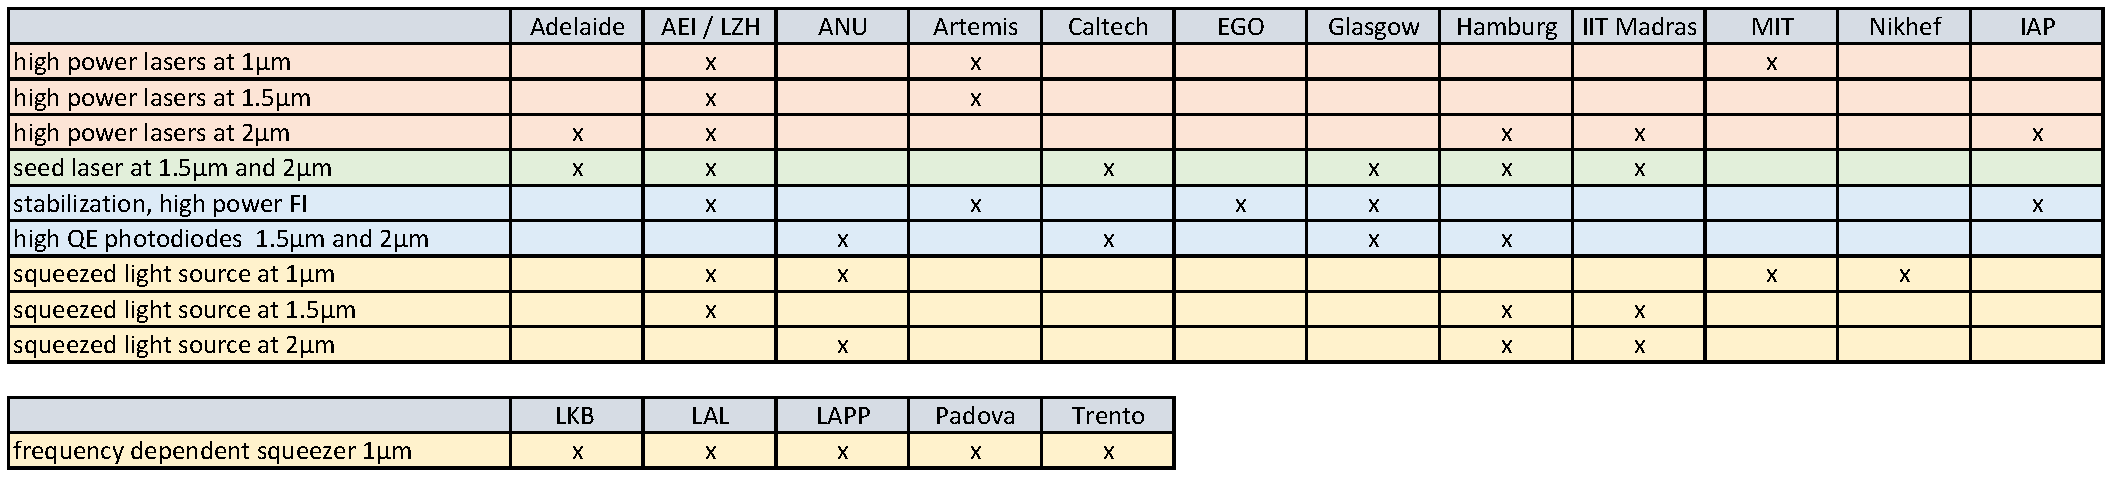
\includegraphics[width=\textwidth]{Figures/Light_source_Fig1.png}
%	\caption{Current or planned R\&D on high power laser and squeezed vacuum sources}
%	\label{fig:LightSourceRD}
%\end{figure}

A survey within the gravitational-wave community showed that more than 10 groups currently perform R\&D on light sources for 3G detectors. All relevant research topics are being worked on by at least two groups. A snapshot of which group is working on which topic can be found at~\cite{LightSource_RD_table}. We also analyzed available documentation and presentations on 3G detectors to extract requirements for the high power lasers and squeezers.

The requirements for the PSL and the squeezed light sources for 3rd generation detectors are not yet well defined. The Einstein Telescope~\cite{ET2011} is planned around a 500\,W laser at 1064\,nm in the spatial $\rm LG_{33}$ mode and a 3\,W laser at a wavelength of 1550\,nm in the fundamental Gaussian mode.
% \greencomment{Dave: It might be good to include a simple summary table of the current knowledge of the requirements for laser performance for ET, CE, and Voyager} \magentacomment{hal: there is some space left at the end of the chapter, so space-wise we could} 
Even though these are clear requirements, the ET design is currently being reevaluated. In particular the operation of the ET high power IFO in the spatial $\rm LG_{33}$ seems questionable. The current Voyager design plans for a HPL with a power of 200\,W and a wavelength of 1550\,nm or longer to minimise absorption in the Silicon test masses. The second phase of Cosmic Explorer~\cite{CosmicExplorer2017}, foreseen to operate at a similar wavelength, will require a HPL with much higher power. This power level is currently not well defined but may be as high as 1\,kW~\cite{GWADW2018,ISWP:2018}. The wavelength choice depends on several factors, such as the availability of high power lasers, absorption of the substrates and the high reflective coatings of the test masses, scattering and the availability of photo detectors with high quantum efficiency. As information on several of these factors is missing, a final wavelength choice can not yet be made. Currently wavelengths of 1550\,nm and around $\rm 2\, \mu m $ and $\rm 2.1\, \mu m $ are targets due to promising high power laser concepts for these wavelengths. Hence R\&D on HPL for three different wavelengths (1064\,nm, 1550\,nm and around $\rm 2\, \mu m $) has to be performed until the final wavelengths are selected. 
No information on PSLs stability requirements for 3G detectors exists at present. As a 10 times better sensitivity is aimed for we assume that the power, frequency and beam jitter stability has to be a factor of 10 higher than in advanced detector PSLs. Concerning the spatial and polarization purity we expect similar requirements as for the advanced detectors.
All 3G detector designs currently incorporate 10\,dB of detected squeezing, meaning that squeezed vacuum sources with squeezing levels of $> 15$\,dB are required.

Thus, in this report we assume that \emph{initially} 250\,W at 1064\,nm and 500\,W at  $ 1.5\, {\rm \mu m}$ or in the $ 2\, {\rm \mu m}$ region will be required. We expect that a factor of 10 less noise compared to 2G PSLs and similar spatial and polarization purity as in 2G PSLs will be needed. Furthermore, we assume that a squeezing level of 15\,dB will be sufficient for \emph{initial} 3G detector operation. For the \emph{final} 3G detectors, we expect that  500\,W at 1064\,nm and 1\,kW at  $ 1.5\, {\rm \mu m}$ or in the $ 2\, {\rm \mu m}$ region again with similar stability and beam purities as in the initial 3G phase will be required. A \emph{final} squeezing level requirement of 20\,dB is assumed.

%\begin{itemize}
%	\item HPL with a power of 250\,W at 1064\,nm with a factor of 10 less noise compared to the 2G PSL and similar spatial and polarization purity requirements as 2G PSLs
%	\item HPL with a power of 500\,W at  $ 1.5\, {\rm \mu m}$ or in the $ 2\, {\rm \mu m}$ region with a factor of 10 less noise compared to the 2G PSL and similar spatial and polarization purity requirements
%	\item Squeezed light sources at all three wavelength with 15\,dB squeezing level
%\end{itemize}
%
%For the final 3G GWD configurations the following PSL requirement are assumed:
%\begin{itemize}
%	\item HPL with a power of 500\,W at 1064\,nm with stability and purity as above
%	\item HPL with a power of 1\,kW at  $ 1.5\, {\rm \mu m}$ or in the $ 2\, {\rm \mu m}$ with stability and purity as above
%	\item Squeezed light sources at all three wavelength with 20\,dB squeezing level
%\end{itemize}


\section{Pathways and required facilities} \label{sec:pathway}
The pathway towards adequate PSLs for 3G detectors has several steps:
\begin{enumerate}
	\item Demonstration of reliable high power generation with required power level, low enough free-running noise (defined by stabilization constraints) and acceptable spatial and polarization purity (functional prototype)
	\item Design, fabrication and test of a HPL according to reproducible fabrication steps with the required diagnostic and stabilization actuators. Demonstration of long-term stable operation and conceptual demonstration of the stabilization concept (engineering prototype).
	\item Final design steps as part of a 3G project and reliability test of the stabilization concept.
\end{enumerate}

\noindent Item 1 is part of generic laser research and is typically performed by university or laser research laboratories. We expect, that up to a power level of $ \approx 200 \, {\rm W} $ this research will be done in the laboratories listed in \cite{LightSource_RD_table}, but new groups may also join the effort. Together with a coherent combination step this work should be sufficient for the 1064\,nm 3G HPL development.
A new coordinated R\&D effort is required to develop a 1\,kW class laser with a wavelength longer than or equal to $ 1.5\, {\rm \mu m}$.
% {\color{red} @Benno: Do we have any idea on how to generate 1\,kW in one step? Or do we need to combine 4 x 250\,W lasers?}
% Benno's answer: No I don't

The reliability and reproducibility part of the engineering step needs a dedicated program of a large laser research lab or industrial involvement. The scope of this step is normally not included in the programs of research funding agencies, so a dedicated R\&D funding program will be required to cover the costs.
Furthermore specific infrastructure and trained staff is required for the fabrication part of the engineering prototype phase. The assembly and stabilization part can be done in one of the laboratories of the GWD community (see \cite{LightSource_RD_table}) or in newly joining laser labs. The same holds true for one or several coherent combination steps. Depending on the progress of the wavelength decision, the engineering prototype step needs to be conducted for two or three wavelengths. During this phase several identical HPLs should be built and characterized in a long term test.

The final design step is part of each specific 3G project and should be performed at an early stage of the respective project with project funding.

The pathway towards an adequate squeezed light source will most likely involve university and research lab based R\&D. The required funding is on a scale that can be covered by regular research grants and the development and improvement of non-classical light sources falls in standard calls of funding agencies. Squeezing levels of $ \approx 15 \, {\rm dB} $ have already been achieved for  $ 1\, {\rm \mu m}$ and  $ 1.5\, {\rm \mu m}$ such that the main technical challenges for these wavelengths are the reduction of loss in optical components and improving the stability and controllability of the squeezing phase. The squeezing research at $ 2\, {\rm \mu m}$ is far less advanced and substantial effort has to be put into the generation of high squeezing levels and low loss components. Several parallel efforts should continue for each wavelength as this approach allows to compare different technical solutions and chose the most appropriate for each project when project funding arrives.

%\subsubsection{functional prototypes}
%Show that high power generation concepts works reliable, accept poor noise performance, missing diagnostic and actuators for stabilization
%\subsubsection*{1064\,nm}
%we assume reliability problem of 200\,W class fiber amplifier will be solved for Advanced detectors (current work at AEI/LZH, MIT and Artemis)\\
%develop coherent combination techniques at 2x250\,W power level
%\subsubsection*{1550\,nm}
%assume AEI/LZH fiber amplifier development is successful
%\subsubsection*{$\rm \bf 2\,\mu m m$}
%assume either Adelaide cryo HM or wavelength doubling of 1064\,nm in OPA is successful
%\subsubsection*{stabilization}
%develop stabilization concepts for all three wavelength adequate for free running noise and available actuators of functional PT developments
%\subsubsection{engineering prototype}
%after final wavelength selection transfer concepts to laser lab or company capable of designing and fabricating an engineering prototype that meets all requirements concerning power, noise performance, spatial and polarization purity, actuators with sufficient range and bandwidth, diagnostic\\
%transfer engineering prototype to research lab for characterization and pre-stabilization\\
%build several engineering prototypes for long-term/reliability tests

\section{Outlook and recommendations}
%\section{Type of collaboration required:  small/large}
%As in the past a strong collaboration between a group within the gravitational-wave community and a laser research lab or industry is required (such as AEI/LZH, Artemis/Alphanov, ICRR/Mitsubishi) to design and build suitable HPLs at the different wavelengths. As the different wavelengths need different solutions, a loose collaboration between the respective wavelength groups would be sufficient. It would be desirable to have at least two collaborations to work on laboratory prototype solutions for each wavelength to explore different concepts and alternative technical solutions. These groups should have a strong connection with regular meetings to exchange results and ideas. This approach would possibly avoid a single supplier problem.
%No particular collaborations are required for the squeezing research. The normal exchange of concepts and results at collaboration meetings and conferences seems sufficient. 
As in the past a strong collaboration between a group within the gravitational-wave community and a laser research lab or industry is required (such as AEI/LZH, Artemis/Alphanov, ICRR/Mitsubishi) to design and build suitable HPLs at the different wavelengths. As the different wavelengths need different solutions, a loose collaboration between the respective wavelength groups would be sufficient.  No particular collaboration arrangements are required for the squeezing research. The normal exchange of concepts and results at collaboration meetings and conferences seems sufficient. 

We recommend that
\begin{itemize}
\item for high power laser development at least two collaborations work on laboratory prototype solutions for each wavelength to explore different concepts and alternative technical solutions.  These groups should have a strong connection with regular meetings to exchange results and ideas. This approach would possibly avoid a single supplier problem.
\item for squeezing light sources, the existing development effort should be maintained, supported by the development of high efficiency photodetectors and required auxiliary optics for two micron wavelength.  
\end{itemize}

Given the long experience in laser development in the GW community, we can lay down a fairly precise roadmap: 

%\section{Road map recommendations}
\subsection*{HPL 1064\,nm}
\begin{itemize}
	\item 2019 - 2020 : continue development and reliability studies of 2G PSL systems at the 250\, W level and perform coherent combination demonstration experiments at high powers
	\item 2021 - 2024 : engineering prototype (see section \ref{sec:pathway}) 500\,W HPL and conceptual test of stabilization and spatial filter solutions
	\item 2024 - ... : final design and fabrication of HPL with the initial 3G requirements within specific 3G projects, in parallel R\&D on path toward the final 3G requirements 
\end{itemize} 


\subsection*{HPL ${\bf 1.5 - 2.1 \, {\bf \mu m}}$}
\begin{itemize}
	\item 2019 - 2021 : identify concepts for a 1\,kW HPL that fulfills the stringent 3G detector HPL requirements (most likely several coherently combined stages)
	\item 2022 - 2024 : 1\,kW HPL functional prototype phase (see section \ref{sec:pathway})
	\item 2024 - 2028 : 1\,kW HPL engineering prototype phase (see section \ref{sec:pathway})
	\item 2028 - ... : final design and fabrication of HPL with the initial 3G requirements within specific 3G projects, in parallel R\&D on path toward the final 3G requirements
\end{itemize} 


\subsection*{squeezed light sources for 3G GWDs}
\begin{itemize}
	\item 2019 - 2026 : continue laboratory based R\&D on squeezed light sources at all wavelength, potentially involve industrial partners to design and fabricate low loss optical components
	\item 2026 - ... : final design and fabrication within specific 3G GWD project
\end{itemize}

\greencomment{Stan: Recommendations (sensible ones) are buried in the Outlook section--possibly rewrite/reformat to bring out the recommendations.  
}

%\subsection{HPL 1064\,nm}
%\begin{tabular}{|p{1.8 cm}|p{10cm}|}
%	\hline 
%	\textbf{time} & \textbf{work}  \\ 
%	\hline 
%	2019-2020 &continue development and reliability studies of 2G PSL systems at the 250\, W
% level and perform coherent combination demonstration experiments at high powers \\ 
%	\hline 
%	2021-2024 & engineering prototype (see section \ref{sec:pathway} ) 500\,W HPL and conceptual test of stabilization and spatial filter solutions \\ 
%	\hline 
%	2024 - & final design and fabrication of HPL with the initial 3G requirements within specific 3G GWD project, in parallel R\&D on path toward the final 3G requirements \\ 
%	\hline 
%\end{tabular} \\

%\subsection{{HPL ${\bf 1.5 - 2.1 \, {\bf \mu m}}$}}
%\begin{tabular}{|p{1.8 cm}|p{10cm}|}
%	\hline 
%	\textbf{time} & \textbf{work}  \\ 
%	\hline 
%	2019-2021 &identify concepts for a 1\,kW HPL that fulfills the stringent 3G GWD HPL requirements (most likely several coherently combined stages)\\ 
%	\hline 
%	2022-2024 & 1\,kW HPL functional prototype phase (see section \ref{sec:pathway} ) \\ 
%	\hline 
%	2024 - 2028 & 1\,kW HPL engineering prototype phase (see section \ref{sec:pathway} ) \\ %
%	\hline 
%	2028 - & final design and fabrication of HPL with the initial 3G requirements within specific 3G GWD project, in parallel R\&D on path toward the final 3G requirements \\
%	\hline
%\end{tabular} \\

%\subsection{squeezed light sources for 3G GWDs}
%\begin{tabular}{|p{1.8 cm}|p{10cm}|}
%	\hline 
%	\textbf{time} & \textbf{work}  \\ 
%	\hline 
%	2019-2026 &continue laboratory based R\&D on squeezed light sources at all wavelength, potentially involve industrial partners to design and fabricate low loss optical components\\ 
%	\hline 
%	2026 - & final design and fabrication within specific 3G GWD project \\
%	\hline
%\end{tabular} \\

%\subsection{Suggested mechanisms}
%annual meetings, keep list of who does what,\\
%team up of GWD projects and funding agencies in engineering PT stage
%\subsection{Impact/relation to 2G and upgrades}
%at 1064\,nm laser development for 2G and upgrades is in direct path to 3G and will serve as long-term test of some concepts

%\subsection{Suggested mechanisms}
%annual meetings, keep list of who does what,\\
%team up of GWD projects and funding agencies in engineering PT stage
%\subsection{Impact/relation to 2G and upgrades}
%at 1064nm laser development for 2G and upgrades is in direct path to 3G and will serve as long-term test of some concepts
\clearpage
%\chapterimage{Figures/speedmeterzoo_filt.png} % copy right: Stefan Danilishin
\chapterimage{Figures1_3/squeezer-1_3.png} %copyright: Harald Lueck
% Chapter heading image
\chapter{Quantum Enhancements}
%\section{Quantum Enhancements}
\label{sec:Quantum}

%\section{Introduction} 
\vspace{1 cm} 
Quantum noise, originating from the quantized nature of light, limits the performance of laser-interferometric gravitational wave detectors over a large part of the observational spectrum. In contrast to many other fundamental noise sources, quantum noise can be strongly influenced and shaped by the interferometer configuration, e.g., the type of interferometer, number of optical components and their masses, mirror reflectivities and optical losses, and the use of additional optical cavities. Advanced interferometer topologies for quantum noise reduction beyond the current state of the art have been proposed~\cite{Danilishin:2019dxq}. Such configurations have the potential to significantly improve the quantum noise in a specific frequency region of interest (e.g. at the low-frequency end for more accurate source parameter extraction or the potential of early warning for signals with an expected counterpart; at the high frequency end for improved neutron star physics) or even to provide a broadband improvement across the full observational spectrum. 
With quantum noise reduction schemes developing rapidly, building additional flexibility and space into the 3G infrastructure is advised to allow for enhancements and upgrades to the initial 3G detectors as technology becomes available. 
%Taking full advantage of the best quantum noise reduction schemes available for 3G will require additional flexibility and space to be built into the planned infrastructure that allow for enhancements and upgrades to the initial 3G detectors. 
Broadly speaking, all advanced quantum noise reduction schemes rely on either the addition of long (up to km-scale) optical cavities (with potentially strongly reduced length noise requirements compared to the main interferometer), and/or major modifications to the optical configuration of the output port, i.e., the optical path between the main interferometer and main photodetectors used for reconstruction of the gravitational-wave signal. 
% Quantum noise reduction results from changes to the whole interferometer, that intrinsically links most subsystems of the observatory. 
The implementation and use of quantum noise reduction techniques can depend on and affect many subbsytems of the interferometer. The associated research and development therefore requires considerable effort, initially with detailed modelling, followed by extensive experimental testing of complete interferometer configurations in suitable environments, covering the entire range from small-scale tabletop experiments to low-noise prototype interferometers. A worldwide coordination of the required R\&D activities will allow an efficient execution of the required research programs and will also support the procurement of the required R\&D funds. 

\section{State of the Art}
The impact of the quantum noise of the light field can be shaped and mitigated by smart optical schemes and interferometer designs. We distinguish between two quantum noise components: shot noise and radiation-pressure noise, which originate from the quantum fluctuations of light and its interaction with the test masses~\cite{Cav1980}. Shot noise is inversely proportional to the square root of the optical power inside the arm cavity, and is dominant at higher frequencies (above 100 Hz in the case of Advanced LIGO); radiation-pressure noise is proportional to the square root of optical power, and is dominant at low frequencies. Radiation-pressure noise is sometimes called quantum `back-action' noise. Due to the Heisenberg Uncertainty Principle, the trade-off between these two, when varying the optical power, leads to the so-called Standard Quantum Limit (SQL). Developing quantum techniques for reducing quantum noise and surpassing the SQL is a very active field of research in the GW community. 
%\pagebreak
% At high frequencies, the 
The influence of shot noise can be reduced by any combination of increasing the circulating laser power, by using squeezed light, by improved readout schemes, or by methods which increase the signal response of the instrument in the frequency range of interest~\cite{StMe1991,Mizuno:RSE1993,Osamu:2006}. High laser power poses a number of technical challenges, including thermal distortions of the test masses and optics which can lead to additional optical loss and parametric instabilities where the resonances of the optics are excited by the light~\cite{BSV2001,Evans:2015raa}. Squeezing is anticipated to be applied for all future observatories, either as the main scheme to reduce quantum noise or in combination with more advanced interferometer schemes. High frequency quantum shot noise can also be shaped by enhancing the detector response in a certain frequency range, but usually this involves a trade-off leading to worse sensitivity outside this targeted band.  

% At low frequencies, the 
Radiation-pressure noise can be addressed by increasing the interferometer test masses and by various schemes adopting aspects of quantum-non-demolition techniques~\cite{KLMTV2001,PuCh2002,Che2003,Braginsky:2004fp}. Theoretical research into radiation pressure noise reduction is very active and has produced a wide range of schemes that show a potential for significant sensitivity improvement. At the same time, table-top experiments on quantum limited systems have become accessible to a wider community. However, the experimental investigations of possible schemes lag behind the theoretical work. We expect the range of interesting options for quantum noise reduction to shrink over the coming years based on result from experimental research at small experiments and prototype interferometers.

Quantum noise beyond the SQL already plays an important role in the Advanced detectors~\cite{BuCh2001}. GEO600~\cite{GEO:Squeezing}, Advanced LIGO~\cite{H1:Squeezing,AdvancedLIGO2015} and Advanced Virgo~\cite{AdvancedVirgo2015} are currently demonstrating and improving squeezed light injection, obtaining shot noise reduction of up to 6\,dB. A+ and Advanced Virgo+ will test frequency dependent squeezing with short (300\,m) filter cavities~\cite{Eva2013,TAMA_FDS2016}, targeting 6\,dB effective squeezing over the whole detection band. Further, balanced homodyne readout~\cite{BHD,Stefszky:Balanced2012} will be part of A+. The lessons learned through these implementations will greatly benefit 3G quantum noise designs.

\section{Requirements for 3G}
Dual-recycled Fabry-Perot Michelson interferometers combined with squeezed light injection are the state-of-the-art for current gravitational-wave detectors and serve as a robust, low-risk baseline design for 3G observatories. More innovative interferometer schemes e.g. speedmeters or variational readout schemes.
% , less researched so far, 
may offer potentially higher quantum noise suppression factors (in particular at the very low frequency end of the detection band, i.e. below 10\,Hz),  but they require further R\&D 
 in order to first evaluate their principal suitability for application in 3G observatories and then to fully qualify and develop them. 
The following list details the top level  key requirements in terms of quantum noise reduction schemes   for 3G detectors:

\begin{itemize}
\item High circulating light power is an essential ingredient in many quantum noise reduction schemes, for example to reduce shot noise, or to make use of correlation effects in opto-mechanical systems. Low-loss and stable operation of interferometers at the several megawatt level   is a key requirement for 3G detectors,  which drives requirements for related subsystems, e.g.  for low absorption coatings, suitable cooling systems for cryogenic interferometers, sufficient thermal compensation schemes and mitigation of parametric instabilities.  .
\item  Long-term  stable,  low-maintenance  and well controllable squeezed light sources (with the laser wavelengths used by 3G detectors, e.g. 1064\,nm, 1550\,nm and $\approx$2000\,nm), usually combined with long (hundreds  of meters to km-scale) filter cavities, implemented to give a quantum noise reduction of  at least  10\,dB  across the full observation band .
\item Efficient implementation of QND schemes and squeezed-light technology relies on  low optical losses. For instance in order to obtain 6\,dB of observed squeezing the maximum loss on the full optical train from the creation of the squeezing up to the detection on the main photodiodes has to be below about 22\,\%. In order to increase the observed squeezing to the envisaged 3G levels of 10+\,dB of squeezing the total losses have to be reduced to below 8\,\% \cite{LSC_IS_WP}. Hence there are very stringent requirements to develop  low-loss optical components such as Faraday isolators (with less than 1\,\% of optical loss) , reduction of optical scattering due to improved mirror surface figure errors, and adaptive optics for 3G detectors  which allow to reduce modematching losses to below 0.3\,\% . 
\item High-quantum-efficiency photodiodes (>99\%) at the operating light source wavelengths (e.g. 1064\,nm, 1550\,nm and $\approx$2000\,nm).
\item Heavy test masses of about 200\,kg,  possibly up to 500\,kg in the case of CE,  to suppress the effect of radiation pressure noise technical control noise and also to accommodate the large laser beams originating from the long baseline of the planned 3G detectors.
\item Adequate low-noise control systems for the main interferometer as well as auxiliary systems like filter cavities and readout system, compatible with astrophysical sensitivity in the sub-10Hz band.
For instance phase noise in the filter cavity control reduces the observable squeezing. For 3G detectors a phase noise level of smaller than 10\,mrads is required \cite{LSC_IS_WP}.
\item There are theoretical approaches to circumventing the SQL to any desired degree, but the limit to performance will always be set by the achievable optical losses in the system. Future R\&D will be able to quantify how the loss distribution and different optical layouts set this limit.
\end{itemize}

%\section{Benefits for 2G} 
%Both 2G and 3G detectors are based on long baseline L- or triangle-shaped interferometers with additional cavities.
%% The fundamental shape of 3G and 2G detectors will be based on long baseline L-shaped interferometers with additional cavities. 
%It is expected that some quantum noise reduction schemes developed for 3G can be installed in current facilities and should be considered for further upgrades to 2G observatories. This will mitigate some risks associated with 3G. However, only 3G facilities will be able to fully support the potential of advanced quantum noise reduction schemes, and quantum noise R\&D for 3G is not a subset of ongoing efforts but demands a new dedicated approach, requiring funding and person power. Challenging R\&D for 3G observatories has the potential to attract additional early career scientists who will be able to also support the needs of the detectors today. 
% (as set out by collaboration agreements).

\section{Outlook and Recommendations}
%\section{Recommendations and timeline}
A significant R\&D effort is required to make an informed selection of the optimal quantum noise reduction strategies for 3G detectors and to enable their risk free application to maximise the science return of 3G 
 observatories. 


The R\&D roadmap in terms of quantum noise improvements for 3G detectors can be divided into 2 broad strands: 1) R\&D to realise the observation of frequency dependent squeezing at the 10+\,dB level. 2) R\&D to evaluate and ultimately qualify more innovative, but so far less developed, QND schemes, which have the potential to further improve the sensitivity of 3G detectors at the low frequency end.  
We recommend the following actions:
\begin{itemize}
    \item Parallel development of low loss optical components (e.g. Faraday isolators with loss of less than 1\,\%) and loss reduction techniques (e.g. for all wavelength currently under consideration for 3G detectors (e.g. 1064\,nm, 1550\,nm and $\approx$2000\,nm) 
    \item Parallel development of high-quantum efficiency photodiodes for 1550\,nm and $\approx$2000\,nm. A global coordination of the communication with photodiode manufacturers will increase the chances of success. 
    \item Development of unified classification scheme of QND techniques and a common approach to analysing and comparing their performances
    \item R\&D programme of table top proof of principle experiments, followed by demonstration in 10\,m class prototype facilities in order to qualify any promising QND schemes going beyond the Dual-Recycled Fabry-Perot Michelson with frequency dependent squeezing.  The quantum noise reduction techniques used for 3G detectors must reach maturity and be demonstrated by prototypes several years before 3G instrument installation.
\end{itemize}
 
 

%\greencomment{Stan:  I would like to see the Outlook section changed to Recommendations and to include more specific recommendations--the one on a uniform classification scheme and a common way to compare different schemes is a good example of such a rather specific rec.
%}
%\subsection{Quantum Noise Reduction Techniques under consideration}
%Quick overview of the most prominent quantum noise reduction techniques currently pursued. Maybe this could be done in a separate explanation box rather 
%than in the main text of the document?
%\subsection{Current State of the Art}
%\begin{itemize}
%\item Dual-recycled, Fabry-Perot Michelson
%\item Injection of squeezed light, obtaining about 4dB max
%\item A+ and Advanced Virgo+ will test frequency dependent squeezing with short (300\,m) filter cavities, targeting 6dB effective squeezing.
%\item Balanced homodyne readout will be part of A+, allowing in principle to change readout quadrature.
%\item Quick list of current losses for 1064nm: QE PDs, Faraday isolators etc.
%\end{itemize}
%\subsection{Requirements}
%Need to start here with a quick discussion on the relation of quantum noise 
%and laser wavelength: To first order quantum noise reduction schemes are independent of wavelength so all the drivers for changing towards longer wavelength come from other noise sources.Hence in the following assume that each of the discussed quantum noise reduction techniques can be realised equally well for any laser wavelength. However, we need to keep in mind that there could  be potential showstoppers, e.g. if it would turn out that there are no high quantum efficiency photo diodes available at 2 micron, which could lead for quantum noise considerations to rule out certain wavelengths.  
%\subsubsection{3G initial}
%\begin{itemize}
%\item \textbf{Result driven: 10\,dB effective quantum noise reduction over 2G for frequencies at mid and high frequency, plus pushing the radiation pressure noise below a few Hertz.}
%\item Current baselines: ET and CE designs are currently based on tuned (ET-HF and CE) or detuned (ET-LF) dual-recycled Fabry Perot Michelson interferometers, with frequency dependent squeezing created with km-scale filter cavities, combined with heavy test masses of the order 200\,kg to reduce radiation pressure noise at low frequencies. 
%\item Alternative approaches: Several alternative approaches are currently researched which provide more cost effective ways to improve the same sensitivity as the baselines mentioned above. Examples include conditional squeezing which uses an EPR measurement for generation of frequency dependent squeezed light and therefore removes the need for long baseline filter cavities; speedmeter interferometers which inherently suppress back action noise.     
%\end{itemize}
%\subsubsection{future}
%No limit. The more reduction the merrier. (Obviously need some better words for this section. Might need to discuss within full committee what level of speculation/optimism one should put in here to make it consistent with the other sections?)
%\subsection{Pathways and required facilities}
%\begin{itemize}
%\item Bench mark parameter set, for evaluation of different quantum noise reduction schemes. 
%\item Dedicated prototype test programmes for full interferometer schemes and low noise tests.
%\item Table top tests of interferometer building blocks, such as low loss optics, high QE photo diodes. 
%\end{itemize}
%\subsection{Type of collaboration required:  small/large}
%\begin{itemize}
%\item From feedback we received from community, the key that is needed is not 
%necessarily more collaboration (though this si also welcome), but rather more coordination, to make sure there are prototype experiments testing all the different promising configurations and we do not miss to develop one. 
%\end{itemize}
%\subsection{Suggested mechanisms}
%\begin{itemize}
%\item Community feedback asked for annual quantum noise workshop with special focus to bring together theorists and experimentalists. 
%\item Prototype coordination (partly happening already via LSC MOUs). Which body would take this on to cover more than just LSC?
%\end{itemize}
%\subsection{Impact/relation to 2G and upgrades}
%\begin{itemize}
%\item 2G consolidates state of the art and test baseline scheme, i.e. frequency
%dependent squeezing. 
%\item Benefit for 3G programme for 2G: Potentially improved sensitivity and faster commissioning plus risk reduction.
%\end{itemize}
\clearpage
\chapterimage{Figures/aux_optics.png} % Chapter heading image
%PMC bench in the 10m AEI prototype copyright AEI
\chapter{Auxiliary Optics}
%\section{Auxiliary Optics}
\label{sec:Aux-optics}

We use the term \emph{auxiliary optics} here for any optical subsystem not otherwise covered by a specific category (e.g. core optics or light sources). We further sub-categorize into these subsystems:
The {\bf Input Optics} subsystem includes all optics between the light source and the input of the core interferometer, typically defined by the power recycling mirror. The {\bf Output Optics} subsystem includes all optics between the core interferometer output (typically defined by the signal recycling mirror) and the photo-detectors which detect the gravitational wave signal, with the exception of specific optical components used for the generation of squeezed light. The {\bf Active Wavefront Control} subsystem includes means for sensing and actively controlling the spatial properties of interferometer beams, with the typical goal of minimizing mode matching losses and contrast defects. The {\bf Stray Light Control} subsystem encompasses all design features which are intended to reduce the impact of stray light on the detector operations. Finally, the subcategory {\bf Other Auxiliary Optics} catches optical subsystems that fall neither into the other larger categories or the aforementioned auxiliary optics subcategories.

\section{State of the art}
The {\bf Input optics} subsystem is responsible for delivering the laser light from the pre-stabilized laser (PSL) system to the core interferometer in the correct spatial mode, with the necessary phase modulation sidebands, as well as with the required frequency, intensity and alignment stability conditions. This subsystem therefore typically includes an electro-optic modulator (EOM) for producing the phase modulation, one or more suspended input mode cleaner (IMC) cavities, a power control system, and a input Faraday isolator (IFI) to protect the PSL from light reflected from the main interferometer. Detailed descriptions of the IO subsystems of aLIGO and AdVirgo can be found in Refs.~\cite{aLIGO_IO} and~\cite{IOchapter} respectively. 

\noindent
In 2G detectors, the {\bf Output optics} subsystem is responsible for filtering out higher-order spatial modes and unwanted control sidebands from the interferometer output light, and delivering the beam to the photodetectors where the GW signal measurement is made. The recent and planned squeezed light upgrades expand the role of this subsystem to include delivery of the squeezed beam to the main interferometer. This subsystem typically includes an output Faraday isolator, an output mode cleaner cavity (OMC), and high quantum efficiency photodiodes.

\noindent {\bf Active Wavefront Control} (AWC) is used in GW detectors to compensate for thermal effects caused by the absorption of light in the interferometer core optics. As the circulating light power goals increased from 1st to 2nd generation detectors, so too did the requirements for compensation of these thermal effects. The 2G detectors have all implemented a range of active wavefront control methods including ring heaters, CO$_2$ laser heating, thermal radiation projection, and thermally deformable mirrors~\cite{aLIGO_AWC, AdVirgo_IO}. This subsystem is often conflated with the thermal compensation system (TCS), although TCS constitutes only a part of the AWC system. 

\noindent {\bf Stray Light Control}
mitigates the effects of light scattered out of the main beam and then scattered back into it as that can cause noise that can limit the sensitivity of the detector.
To address this problem, many precautions are taken in GW detectors to minimize the amount of light scattered out of the beam (by using high-quality smooth optical surfaces everywhere), and also to minimize the available paths for re-entry of scattered light into the main beam (by using baffles wherever possible). 

\noindent 
Examples for the category {\bf "Other Auxiliary Optics"} include auxiliary length sensing (ALS) systems for pre-stabilizing the arm cavities, and optical levers for local sensing of the alignment of optics.

\section{Requirements, challenges and current/planned R\&D}
\subsection{Input optics}
 % Future 3G GW detectors will require different input optics than the current second-generation detectors. 
 The ways in which the 3G detector input optics will differ from the current ones depends heavily on some of the design decisions for 3G detectors, many of which have not yet been made. Most critical for the input optics will be the choice of laser wavelength; the EOM and IFI rely on unusual electro- and magneto-optic materials that may have significantly different characteristics at longer wavelengths. Choosing suitable materials is not expected to pose a great challenge if the wavelength is changed to 1550\,nm, but 2+$\mu$m will probably require considerable effort. The high power transmitted through these optics makes low absorption critical (due to the resulting thermal lensing and depolarization effects), thus further narrowing the choice of suitable material. At 2$\mu$m Faraday isolators already exist~\cite{EOTFI}, but a high power vacuum compatible one must be developed as it is not commercially available. Iron garnets should be considered as potential candidates for the magneto-optic material for 2+$\mu$m light, also having the advantage that the Faraday rotation effect is an order of magnitude larger than that of TGG in the near infrared range, allowing a reduction in magnet size and the overall footprint and weight of the device.
The IMC design is not expected to fundamentally change beyond the 2nd generation.  However, AdVirgo and aLIGO have both seen that noise contributions have been limited by beam jitter~\cite{aLIGOjitter,adVirgojitter}. Increasing the IMC finesse or adding a second IMC in series with the first could be a way to further suppress the beam jitter. Another possibility is to reduce the beam jitter at the source, either passively or with high bandwidth control loops.  

In addition to upgrades and modifications of existing IO components, several new components are also being researched. High bandwidth electro-optic beam deflectors could be used as actuators for beam jitter suppression loops and for providing alignment sidebands for an alternative method of alignment sensing in both the IMC and in the core interferometer~\cite{RFJASC}. The use of higher-order modes for coating thermal noise reduction is still under consideration for 3G interferometers~\cite{LGmodes}. If this technology is pursued further, the higher-order mode conversion/preparation path is likely to be incorporated into the IO remit. 

The use of complex modulation~\cite{complexmod} and parallel modulation~\cite{kagraMZI} are also under investigation for reducing sidebands-of-sidebands effects that may limit interferometer sensing and control performance.

\subsection{Output optics}
With all 3G concepts assuming significant enhancement from the use of squeezed light, the critical feature for the 3G output optics will be ultra-low optical losses~\cite{squeeze_lossbudget}. OFIs with reduced optical losses are being developed~\cite{EGOLLFI,UFLLFI}, for use in the advanced GW detectors. Figure~\ref{fig:AdVLLFI} shows the low-loss OFI which has recently been installed in Advanced Virgo. OMCs must also be designed for high throughput, and photodetectors must have high quantum efficiency (QE). High-QE photodetectors at longer wavelengths has been identified as a crucial R\&D task; one which may be especially onerous for 2+$\mu$m light. Frequency dependent squeezing will also require the inclusion of a filter cavity (FC) in the path between the squeezed light source and the OFI. 300\,m long FCs are planned for the near-term upgrades to aLIGO and AdV, following on from R\&D performed at MIT~\cite{MITFC} and in Japan\cite{TAMA_FDS2016}. Alternative readout schemes such as balanced homodyne detection (BHD - another project planned for inclusion in A+) will require a redesign of the output optics chain~\cite{BHD}. There is also a need to develop robust length and angular control schemes for detuned filter cavities.
% and finesse control to control pole frequency.

%\begin{figure}[htb]
%\centering
%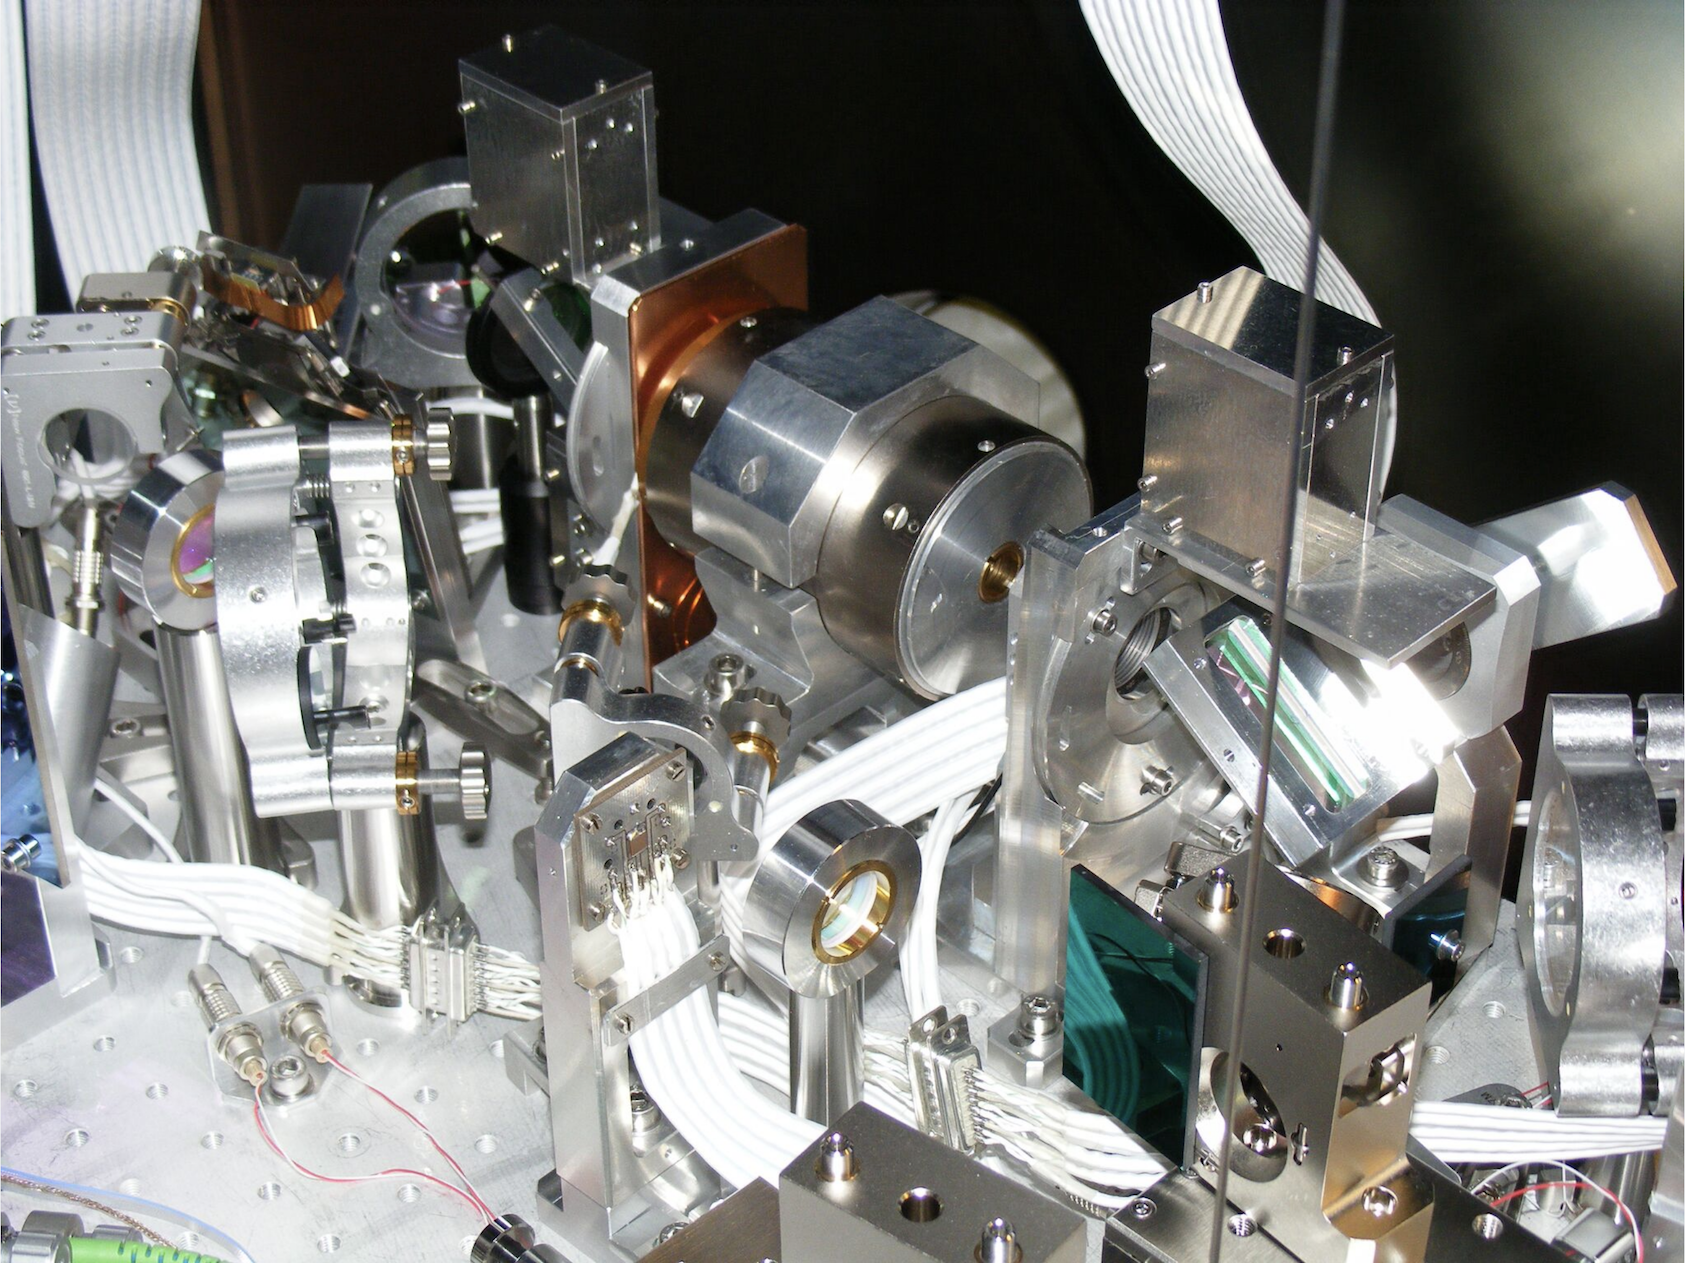
\includegraphics[width=0.6\textwidth]{Figures/LLFI.png}
%\caption{The low-loss OFI upgrade to Advanced Virgo, recently installed ahead of the third observing run of the advanced detector era.\label{fig:AdVLLFI}}
%\end{figure}\magentacomment{Do we want to have this figure here. I does not add much information and is the only figure in all chapters; except intro. On the other hand it would not shorten the chapter, as it does not gain a full page}
\subsection{Active wavefront control}
In 1st and 2nd generation detectors, active wavefront control (AWC) has often been implemented in something of an \emph{ad hoc} way. In no cases has a feedback loop been used to maintain mode matching in a detector during normal operations. This is partly due to the low bandwidth of the typical actuators, but also due to the limitations in the AWC sensors available. As a result, AWC is typically employed in a set-and-forget manner, which requires frequent manual retuning as the circulating power in the interferometer changes. 3G detectors will likely require higher performance from the AWC subsystem for several reasons: higher circulating powers, larger thermal gradients under cryogenic operation, larger beams with flatter wavefronts, and stricter requirements on optical losses. An LSC white paper on AWC has been written to track the LSC R\&D in this direction~\cite{aLIGO_AWC}, and similar work is planned for AdV+. AWC R\&D for 3G detectors is expected to focus on new sensors (RF bullseye wavefront sensors~\cite{bullseye}, improved Hartmann wavefront sensors~\cite{HWS}, phase cameras~\cite{phasecam}), as well as actuators (converting existing actuators for new optic materials, and developing new actuators). 

\subsection{Stray light control}
Although it is often difficult to diagnose directly, stray light was expected to be  limiting the sensitivity of both aLIGO and AdVirgo during O2. As such, improvements must clearly be made in order to reach 3G sensitivities with any methods other than extending the baseline length. Continued R\&D into mirror polishing and coating techniques to give improved surface roughness will go some way to reducing stray light contributions, as will the development of better baffling materials with lower reflectivities. One concern is that if the laser wavelength is changed to 2+$\mu$m, finding good absorbers for baffle materials may become more difficult. 

\subsection{Other auxiliary optics}
AdVirgo, aLIGO and Kagra all either use (or provision for) an auxiliary length sensing system in order to make the interferometer locking process deterministic. Since the optical layout of 3G detectors is not expected to reduce in complexity, it seems natural that similar systems will be required in the future. Optical levers are  omnipresent in 2G detectors, and provide important information about angular motion of the optics. Increased sensitivity in these local sensors may be beneficial for 3G detectors with increased baselines and sensitivity goals, and accordingly R\&D is ongoing towards that end. Suspension point interferometry (SPI)~\cite{SPI} may be a useful technique for reducing low frequency control noise in 3G detectors, and will require an additional auxiliary optical subsystem. SPI is currently being used at the AEI 10\,m prototype interferometer.   

\section{Current R\&D activities, pathways, required facilities, collaborations\\ and mechanisms}
A survey of research groups who are known to be working on, or have previously worked on auxiliary optics topics has been conducted~\cite{AuxActivitiesTable}.

Much of the auxiliary optics subsystems R\&D, such as materials investigations for EOMs and FIs, can be performed in small laboratories. 
Some of the larger subsystems such as filter cavities, on the other hand, require larger integrated facilities for testing. In many cases, the development of 3G auxiliary optics technologies is also beneficially incorporated into the modernisation of second-generation detectors. By virtue of being \emph{auxiliary}, modular, incremental upgrades in many of these technologies are possible. Modular upgrades are not feasible in the case of a change in the main laser wavelength, however. Such a change for 3G detectors will necessitate a broader range of auxiliary optics R\&D, which would benefit from a more complete demonstration on prototype detectors or finally at full scale in LIGO Voyager.

\subsubsection{\bf Input optics} The groups working on IO for 2nd generation upgrades and beyond are primarily those groups who have worked on providing input optics for aLIGO, AdVirgo, GEO and Kagra in the past. In the LSC-Virgo collaboration information is shared on progress in development of future input optics mostly through the auxiliary optics working group, with talks and posters at collaboration meetings. This method of collaboration seems to be sufficient for now. If the community steers towards a change in wavelength, however, additional information exchange mechanisms may be required in order to accelerate the development of suitable input optics components.

\subsubsection{\bf Output optics} The main feature of upgrades of the second generation output optics and beyond is the minimization of optical losses while adding further subsystems such as filter cavities and balanced homodyne detection paths. 
Low-loss Faraday isolators are advantageous for short-term 2G detector upgrades, so it may be useful for the 5 identified groups to work together and hold dedicated workshops to discuss progress and plans in the near future. 
\subsubsection{\bf Active wavefront control} 
This subsystem was identified by the authors as one that could benefit from increased global cooperation. Due to the \emph{ad hoc} nature of the development of this subsystem to date, many groups have taken individual paths to different but often similar solutions. We propose to contribute by forming an active wavefront control subgroup to focus efforts on a common goal of appropriate wavefront sensors and control strategy for future GW detectors. 

\subsubsection{\bf Stray light control} This subsystem could benefit from the collaboration between groups worldwide if the laser wavelength chosen is the same for all of the next generation GW detectors. If different choices are made, each project should organize R\&D activities on their own. From the stray light control perspective at least therefore, significant savings in time and money could be made by choosing common wavelengths between 3G detectors. 

\subsubsection{\bf Other auxiliary optics} Unless required by groups working on auxiliary optics topics outside the scope of the aforementioned, specific collaboration mechanisms are not seen as a priority at this time. 


\subsection{Collaborations between AO and other subsystems}

\paragraph{\bf Light sources} Many of the auxiliary optics subsystems will be strongly impacted by the choice of laser wavelength. Beyond this, the input optics has a direct interface with the light source, and so information exchange between groups performing R\&D in these two areas will be critical.
\subsubsection{\bf Quantum noise} The output optics subsystem will be closely linked to the quantum noise working groups as squeezing is foreseen in all future detectors. Close collaboration between these groups will therefore be beneficial.

\magentacomment{hal: timelines???}

\clearpage
\chapterimage{Figures/Controls2.jpg} % Chapter heading image
% Michelson Model copyright Andreas Freise
\chapter{Simulation and Controls}
\label{sec:Sim_Controls}

Interferometric gravitational-wave detectors are complex optical and mechanical systems. Their core instruments, Fabry–Perot and the Michelson interferometers, can be used for high-precision measurements only if their parameters, especially their base length, is careful controlled. 
The complete detector can have a large number of control loops for the various mirrors and beamsplitters, their suspension systems and many other components, such as the laser, active vibration-isolation systems. The \textbf{Simulations} section lists the requirements for modelling tools for design and commissioning of the complex opto-mechanical interferometers and the \textbf{Controls} section outlines the research required for developing adequate control schemes for future detectors.

\section{Simulations}
\subsection{Current approach to interferometer modelling}
GW detectors require detailed modelling for design and performance studies; this also applies to some extent to prototype experiments (table-top and 10\,m scale). The detector behaviour cannot be modelled with commercially available optical simulations as our requirements differ significantly from those of conventional systems. The proposed third-generation detectors include either new technologies or envisage pushing detector parameters closer to their limits. 
A specific set of tools has emerged that can be used to classify the most commonly used software:

\noindent{\textbf{Time-domain models}} describe the optical field and the optical components in the time domain, i.e. direct outputs will be signals over a discrete time step. Typically the time-domain models are the most powerful   simulations because they can include non-linear and dynamic behaviour.
The disadvantage, however, is that such simulations require significant computing power. Example software: SIESTA~\cite{SIESTA}, E2E~\cite{e2e_2000}.

\noindent{\textbf{Frequency-domain models}} are based on the approximation that the entire system is in a steady-state with only small disturbances or slow (quasi-static) changes. All the modelled features are linearised.
%, thus the system can be described as a set of linear equations. 
This approach provides very fast and flexible models but obviously lacks the ability to model non-linear physical features. Frequency domain software can be further split
into two categories: \emph{FFT propagation} codes and \emph{modal models}.

\newpage

\noindent{\textbf{FFT propagation models}} have been developed to analyse the behaviour of optical fields in the presence of wavefront distortions by discretizing the transverse complex amplitude of the field on a 2D grid.
%The name of this method is derived from the fact that this field can be propagated efficiently using a single two-dimensional discrete Fast Fourier Transform. 
Example software: SIS~\cite{SIS}, OSCAR~\cite{OSCAR}, DarkF~\cite{DarkF, Vinet92}.
 
\noindent{\textbf{Modal models}} use Gaussian modes to describe the spatial properties of the beam, its propagation and scattering. The modal model expands the beam shape into orthogonal modes ordered by spatial frequency forming a complete basis. Thus for near perfect Gaussian beams only a few numerical values describing the mode amplitudes need to be computed resulting in faster simulations. The commissioning of advanced detectors, as well as the design of further upgrades have shown that such tools have become crucial to understand interferometer limitations. 
%Modelling tasks related to alignment sensing and control, parametric instabilities, or simply the effect of mode mismatch or beam clipping on the control systems and ultimately on the gravitational wave signal have taken center stage. 
Example software: Optickle~\cite{Optickle}, \textsc{Finesse}~\cite{Finesse, Freise04}, MIST~\cite{MIST}.

\noindent{\textbf{Interferometer noise calculators}} are configuration level simulations that operate at a higher level so that a given optical configuration is symbolically computed and parameterized. 
%While inappropriate for detailed simulation of the optical plant, 
This approach is very effective for an initial exploration of a parameter space for a variety of optical configurations and for providing simple reference noise budgets. Example software: GWINC~\cite{GWINC}.

\noindent{\textbf{SimPlant}}, a virtual interferometer for commissioning: the commissioners can click a button to turn the machine over to Sim Mode, and then use the usual tools to measure, for example, the noise and transfer functions. This provides the fastest way to compare our theoretical knowledge with the real instrument.
%and see where the differences are. 
The simulated interferometer runs in real time within the real time control system so that the usual controls system can be run. Whether the interferometer being controlled is real or virtual is transparent to the control room operator.

\noindent{\textbf{Ray tracing}} tools are used to find the exact position of beam axes and Gaussian beam parameters in real systems and can help with stray light investigations, often using computer-aided-design (CAD) data from the design of the instrument's mechanical components as a basis. Example software: IfoCAD~\cite{IfoCAD, kochkina}, OptoCAD~\cite{OptoCAD}.
%For scattered light analysis, it is critical to use non-sequential ray tracing and Monte-Carlo methods in order to accurately represent the large dynamic range of field amplitudes necessary to compute the phase and amplitude noise.

%%% -------------------------------------------------------------------------
\subsection{Requirements}
\label{sec:Sim:Req}
%Simulation tools are strongly defined through the context in which they are used. 
Many of the priorities for the research and development of technologies and instrumentation directly translate into a priority task for modelling work or a required effort in developing new capabilities for simulation tools. 
% The main challenges will be the operation at very high circulating power (several MW), the mitigation of excess noise from feedback and control system at low frequency, and the reduction of optical loss and scattered light. Quantum noise reduction schemes will most likely have the strongest impact on the interferometer design. Newtonian noise reduction will be required. 
Significant support from interferometer modelling will be needed for tasks including:
\begin{itemize}
\item High-power operation at low optical loss.
%Small asymmetries in absorption can increase the effective optical loss for squeezed states.
Modelling of squeezed light in higher-order modes, improved thermal compensation systems, improved arm and mode matching techniques.
%\item Parametric instabilities control, modelling of acoustic mode dampers, development of a control scheme that allows tracking and selective damping of a large number of modes, requires more detailed modelling to predict individual modes.
\item Scattered light control, modelling of backscatter of detection optics and interferometer scatter. Include injection of noise with specific coherence into interferometer modelling tools. Non-sequential ray-tracing. Monte-Carlo methods.
\item Control design: better models of control schemes can be achieved by developing more effective tools for the analysis of in-loop cross coupling of a mixed mechanical, optical and electronic system, and for the analysis of modern
control strategies.
\item Advanced quantum noise schemes, development of a robust 'fundamental' quantum limit. Modelling of quantum correlations through complex MIMO (multiple in, multiple out) systems.
%\item Modelling of non-linear optical elements, such as crystals (squeezing), active opto-mechanical elements (unstable filters) etc.  Development and implementation of realistic linearised couplings for these elements into optical models.
\item Study of optical configurations which rely strongly on polarisation schemes, requires the addition of light polarisation to interferometer models.
\item Newtonian gravity noise reduction, advanced modelling of local sensing and global control strategies, require an advanced implementation of mechanical systems and seismic and gravitational noise coupling in interferometer models as well as the simulation of gravitational noise based on ground noise measurements.
%\item Investigation of alternative beam shapes for thermal noise reduction, modelling of auxiliary optical systems to study feasibility.
\item A missing piece in detector simulation is a comprehensive mechanical simulation tool for the vibration isolation and suspension design which includes the capability to handle a variety of mechanical systems and the ability to compute thermal noise for any given configuration.
\end{itemize}

%%% -------------------------------------------------------------------------
\subsection{Impact on detector upgrades}
Interferometer simulations tasks for upgrades of current facilities and for third-generation detectors are closely related and strongly benefit from each other. Simulation tools and interferometer modelling have to be advanced ahead of time in order to be able to provide the essential
support during the design and instrument development. The design of the advanced detectors triggered the development of new tools which then had a significant impact on the commissioning of the first generation. At the same time the interaction with commissioners (and scientists developing advanced detector
technology at prototypes) provided essential community interaction and feedback that resulted in tools with better capabilities, validated test results and expert users. The same synergy is expected now between advanced detectors and 3G observatories; it should be encouraged and utilized as much as possible.

%%% -------------------------------------------------------------------------
\subsection{Recommendations}
To address the above challenges, the current portfolio of software tools must be updated, either by extending the existing software or by providing new dedicated tools. The detailed list of code changes or required features goes beyond the scope of this document. The following are recommendations for the higher-level actions to support an effective and open environment for this effort.

\noindent{\textbf{Additional software}}
Most of the required modelling tasks can be performed by extending and updating the available tools, some of which is already well underway. However some missing functionality might be better achieved by developing new software. Needed packages include an easy to use and flexible time-domain simulation, a 3D beam tracing software dedicated to ground based detectors and a comprehensive modelling software for various suspension systems capable of computing the thermal noise of all elements. In addition, commercial tools should be reviewed to understand when these are superior to custom made tools, for example, for more common optics tasks such as modelling stray light.

\noindent{\textbf{Resources}}
We encourage institutions to increase support for the development and use of simulation tools over the next 5 years, a crucial time for the design of 3G instruments, and for upgrades to current detectors.
%, while the commissioning of detectors will push the limits of current technology. 
Experience has shown that
individual post-docs and PhD students can provide effective tools that are quickly adopted and used by a wide community. However, those tools often come only with rudimentary or outdated documentation and code reviews or formal testing of simulation results are not common practice. We recommend additional, dedicated post-doc support in this area to mitigate this.

\noindent{\textbf{Collaboration and coordination}}
Coordination between research groups and projects is important in three ways:
code development is often done by few individuals in each project who will benefit from having a forum to discuss priorities as well as technical challenges. The same is true for the collaboration between people
%undertaking the code development and those 
doing modelling, often 
%Modelling tasks (design or commissioning) are often 
investigating a new or not-understood behaviour;
collaboration with other scientists investigating similar or related aspects has been shown to greatly reduce the time to reaching a conclusion. We recommend to continue (or establish) working groups dedicated to the interferometer modelling within projects and 
%for these working groups 
to organize workshops/meetings adjacent to international meetings.

\noindent{\textbf{Software and code distribution}}
Accessibility of the software, and ideally the source code, should be improved. Each software tool should have: a) an active maintainer who is responsible for the current code base and who can be identified and reached by any users of the software, b) a single, discoverable web page hosting the master version of the tool or code under a clear and permissible software license, c) documentation about the implemented models and their limitations, including descriptions of mathematical algorithms, or parameter sets used and d) training material, such as a set of examples and tutorials for new users, especially graduate students. Where possible (without breaking existing compatibility) the adoption of common  input and output formats, for example, for files storing interferometer parameters  should be encouraged.

The effectiveness of specific tools is often not defined by the a single feature but by a network effect based on many factors. Any tool benefits greatly from a large user base, for example, through receiving bug reports and the availability and diversity of examples as well as experts on how to use the specific tool. And the impact of a modelling tool is improved significantly by a strong track record and trust by the wider community. We recommend that software maintainers adopts the aim of making the software as accessible as possible without compromising its core functionality. %Similarly we recommend that groups distributing software make an effort in providing training material or training opportunities for new users. The quality and effectiveness of simulation tools can be greatly enhanced by a large and informed active user base.

Those software tools that aim at providing standard results for the wider community must also provide the official data sets or model files, such as, for example default LIGO models for \textsc{Finesse}. The GWINC software package should provide standard noise budgets for all envisaged detectors and the
collaborations should establish a mechanism to review its noise models by the international community.

\noindent{\textbf{Source code maintenance}}
Some important simulation tools date back to their original development in the 80s and 90s. Given the rapid development of computing and computer languages, it could be beneficial to re-implement these in modern frameworks. At the same time the experience and knowledge acquired with the originals should not be lost in the process. A careful development process and code design that finds a balance between modern technology and backwards compatibility
is recommended. Some codes, such as \textsc{Finesse} and GWINC are currently undergoing such a process. Other software should be reviewed for similar updates.

\section{Controls}
\label{sec:Controls}
Control systems are a fundamental part of all interferometric gravitational wave detectors. The optical and interferometric methods used to achieve the strain and displacement sensitivity required for gravitational wave detection are all non-linear; actively nulling the signal with a feedback control system linearizes the output. The control system thus enables the low noise, stable, and linear operation of the detector in the presence of seismic, acoustic, and radiation pressure disturbances.
The detection of gravitational waves poses stringent requirements on the operations of the feedback and feed-forward control systems.
In the past, meeting these requirements has proved extremely challenging.
This is partially because the detectors were designed without sufficient consideration of the controls challenges, and partially because the controls challenges are so extreme and gravitational wave detectors so unique in the field of controls.
Some plans for future detectors aim to strongly improve the sensitivity at frequencies below 10\,Hz. This frequency region is currently dominated by excess noise associated with control systems, and the envisaged noise reduction represents a significant challenge for the control system design and implementation.

\subsection{Current approach}
Considering only the core optical interferometer, gravitational wave detectors have many degrees of freedom,  including the differential arm motion (DARM), which is sensitive to gravitational waves, and many auxiliary degrees-of-freedom, which are not. DARM must be stabilized to linearize the signal, and the many auxiliary degrees-of-freedom must be well stabilized to avoid coupling noise into the gravitational-wave readout. Achieving this second requirement is the primary challenge, due to the large number of coupled degrees-of-freedom, where the couplings may be both non-linear and non-stationary, and the variety of timescales involved (which range from seconds to hours).

In most cases, classical control methods are used to minimize some quantity, typically pole-zero based linear filters in feedback or feedforward systems.
The filter design is based on modelled or measured response functions of the respective degree of freedom (composed by optical, mechanical and electronic parts). There is often a trade-off between robustness of the control loop and the overall sensitivity of the detector.

There are a also few examples of the implementation of more modern techniques:
\begin{enumerate}
\item  Global feed-forward of seismic noise to platforms and suspensions.
\item  $\mu$-Synthesis approach for limited angular control
\item  Feed-forward sensor noise subtraction (removal of seismic noise from wave-front sensors)
\item  Parametric instability damping by phase-locked loops and damping through aliasing of high frequency signals.
\end{enumerate}

\subsection{Requirements}
%\begin{enumerate}
%\item
{\bf Low noise operation:} all control systems must be able to operate on the main and auxiliary degrees of freedom without introducing additional noise. This is a point often missed in design studies, where only ``fundamental'' noises are considered (for example thermal noise, quantum noise, etc.). However, different design choices of the interferometer translate to different requirements for the control system. As an example, second generation detectors are still limited in the low frequency range by (mostly angular) control noise. This is directly related to the interplay between performance the of suspension and seismic isolation design and the trade-off between stability and low-noise in angular controls. If all suspension and seismic platform resonances could be moved to lower frequencies, and if the residual motion at the microseism could be reduced by the seismic isolation, then all angular control systems could be relaxed, improving the low frequency noise of the detectors. Research is required to understand how best to integrate realistic controls limitations into interferometer designs.\par
%\item
\noindent{\bf Non-linear lock acquisition:} the term 'lock' refers to a stable state of the control systems in which all relevant degrees of freedom are stable at their nominal operating position. In the uncontrolled state the interferometer is a highly non-linear system, in the sense that all the optical signals that can be used to estimate the resonance conditions depend in a complex non-linear way on the relative mirror position. The lock acquisition scheme is an algorithm designed to bring the system in a deterministic way from the uncontrolled state to the final low noise state. There is significant room for improvement in this area, since all lock acquisition strategies developed so far are somehow sub-optimal. An example of a design choice that resulted from prototype research and vastly improved the lock acquisition process is the installation of the arm-length stabilization in Advanced LIGO~\cite{Mullavey:12}. The use of similar techniques and modern control theory could improve upon the current lock acquisition scheme. Having a fast and reliable lock acquisition strategy can reduce the down time of the detector.\par
%\item
\noindent{\bf Robustness:} control systems must be able to withstand external perturbations due to environmental disturbances, such as earthquakes, without losing lock and with minimal reduction in sensitivity. Any loss of control translates directly into downtime and a reduction of the observed time-volume. Understanding the mechanisms by which earthquakes cause detectors to lose lock, developing controls system states which might be able to ``ride out'' earthquakes, and developing methods to quickly transition from a low-noise state to a robust state all require further research.\par
%\item
\noindent{\bf Noise cancellation:} feed-forward and linear stationary noise cancellation are techniques already implemented routinely in second generation detectors. However, as those techniques reach their limit, the residual noise couplings are bound to be either non-linear or non-stationary. Development of control strategies to cope with such systems is needed. For example, new methods based on machine learning are a promising avenue to explore to develop such strategies.\par
%\item
\noindent{\bf Optimisation:} In the currently operating detectors, the controls systems are tuned manually, which yields sub-optimal results.  Considering the large number of coupled degrees-of-freedom and the long timescales involved, brute force explorations of the parameters is also impossible. The following all need to be developed or modified to suit the unique needs of gravitational wave detectors: systematic methods to explore the parameter spaces of control systems; robust automated filter design; optimal multiple-input multiple-output sensing, control, and system identification methods. These will likely require combination of offline analysis of data collected while the plant (the gravitational wave detector) is controlled in a non-optimal way, coupled with sophisticated simulations, and carefully chosen sets of test parameters that sample the global parameter space.
%\end{enumerate}

\subsection{Impact on detector upgrades}
Ongoing commissioning of current detectors includes the improvement and optimization of the control systems. We expect that many if not most new control techniques or ideas will be tested and implemented in 2G interferometers first. However, this is not true for schemes that require a very different sensing or actuation approach.

\subsection{Recommendations}
Control noise, or cross-coupling of fundamental noise through control channels, has historically limited GW detectors, especially at the low-frequency end of the measurement band. The requirements of 3G detectors will pose a great challenge to control systems. Control schemes should be developed and tested early as an integral part of detector designs. Synergies with commissioning and detector upgrades should be sought out. At the same time, care should be taken that sufficient theoretical work and tests at prototype interferometers are performed for new control designs that cannot be tested with current detectors.

\clearpage
\chapterimage{Figures/summary.jpg} % Chapter heading image
% Blackboard scribbles copyright Andreas Freise
\chapter{Summary}
\label{sec:Summary}

Prioritize R\&D items by timelines and complexity (Infra and Fac most urgent, solutions known, large cost saving potential), 
Coatings and 3G optics (no clear path forward but a little less time critical) 

\magentacomment{Josh: Here I pasted some remarks from quantum noise that Dave suggested be moved to general considerations.} 

\begin{itemize}
\item National funding agencies to increase funding (staff and instrumentation) of the relevant lab activities and to enable the required long-term research programmes at the relevant prototype interferometers.
\greencomment{Dave: Certainly.  But this is a generic recommendation in the sense that all R\&D 3G efforts need more R\&D funding.  I don't think this needs to be here (or in any other chapter), but somewhere in the main set of recommendations.}
\item Existing GW collaborations to take ownership of 3G R\&D and integrate it into their programs and deliverables, in order to ensure sufficient support for the long-term future of the field (as it has been done so successfully for 2G R\&D during the operation of the initial detectors). 
\item Establishment of worldwide discussion and coordination forum (meeting several times a year) across all relevant collaborations, in order to stipulate exchange of ideas and allowing (if deemed useful) for a coordination of the person-power intensive experimental activities.
\end{itemize}

\section{collection of recommendation section from the various chapters}
\subsection{Facilities + Infrastructure}
collaboration with high energy particle physics community (know-how in building large vacuum
systems from accelerator facilities)

3G Infrastructure and facilities construction will start roughly 5 years before the installation of detector hardware, hence the timescales for technical readiness are shorter and more critical here.
If site preparation for the Einstein telescope is to start as early as $\sim$\,2025 the respective R\&D and detailed technical studies have to start immediately. Respective international and collaboration overarching working groups should be initiated right now.

\subsection{Core Optics}
There is not a research laboratory that is dedicated to develop and optimize the large size crystal growth with the specifications imposed by the GW detectors. This could have a severe impact on the development of 3G detectors.
\magentacomment{hal: The lead times for this R\&D are huge. Steering the direction needs decision points well ahead of time. }
timelines missing
\subsection{Coatings}
By far the most pressing timeline is for the enhanced 2G detectors. In the case of a+LIGO, allowing for a one-year pathfinder after the coating material and process are identified, the required research to identify a suitable mirror coating should be completed by May 2020. This timeline implicitly assumes that the coating will be a sputter-deposited amorphous doped oxide, perhaps deposited at an elevated temperature, a slower than conventional rate and/or with a higher than conventional annealing temperature. It is unlikely that there is time in such a schedule to identify coatings and develop the required equipment for a process with more significant deviations from current deposition methods.

In recognition of the fact that meeting the enhanced 2G detector timeline requires doing basic research on a development schedule, the efforts of the LSC community are of necessity focused on these mirrors. That said, it is also recognized that the community shouldn't put itself again in such a situation, so a portion of the current research effort is devoted to establishing approaches to mirrors for 2.5G and 3G detectors. It is difficult to set research timelines for this effort, since the funding and construction schedules for these systems are not yet established. Another open question is the deposition process that will be required for the 2.5G and 3G mirrors; the further that process is from conventional IBS, the longer it is likely to take to develop suitable tooling. It seems that in any plausible scenario at least five years are available for research into the best approach to mirrors meeting 2.5G requirements. Results for these 2.5G mirrors will, in turn, inform choices with respect to 3G mirrors. It is therefore too soon to argue for a large investment in scaling deposition tools alternative to elevated-temperature IBS for 2.5G and 3G mirrors. That said, as the funding trajectories and interferometer architectures become better defined, it will be important to regularly re-evaluate the current understanding of potential mirror technologies, and make critical decisions, especially with respect to deposition tools with long development times and requiring major financial investments.

\subsubsection{Recommendations}

\noindent The additional funding provided by the CCR for U.S. efforts in coating research, combined with the previously existing NSF support, leave these efforts with reasonably adequate funding in the near future. It would be helpful to add another deposition group to the effort, as there is currently more capacity for characterization of properties (other than cryogenic mechanical losses) than for synthesis. It is also important that the LIGO Lab continue with at least its current effort level, as their contribution to high-throughput mechanical loss characterization, optical scatter and homogeneity measurements, and their overall coordination of sample fabrication, distribution, and characterization is important to the LSC efforts.

In GEO, there is growing capacity for depositing coatings at Strathclyde, UWS and Hamburg. These coatings can be produced at a rate faster than it is possible to characterize their properties at cryogenic temperatures, and thus more resources devoted to such characterization are desirable. Currently, a novel type of ion-beam sputtering is being developed and tested at Strathclyde. While this is a promising research route, there are also plans to set up a large chamber with an industry ion source which should be capable of producing large and uniform enough coatings. This is an important priority in gaining access to more coating facilities which are suitable for the deposition of large, high-quality coatings. Initiating studies of GaP/AlGaP crystalline coatings, using hardware now installed in an MBE chamber at Gas Sensing Solutions Ltd, is also planned. This is an important parallel research direction to the development of amorphous coatings.

In VIRGO, the activities are progressing at the pace compatible with the funding available from other projects. \magentacomment{Josh: I do not understand what the previous sentence intends to say.} LMA and University of Sannio are able to provide high quality coatings at a rate higher than the existing characterization capability in VCR\&D. The project ViSIONs takes care of only one specific aspect of the research, that is the impact and the understanding of deposition parameters on the coatings properties.

At present, there is only one institution, LMA, capable of depositing coatings of a size and quality suitable for gravitational wave interferometers. LMA will continue to be supported as a research and coating facility for future GW detectors by the French CNRS through EGO, while support for another institution, CSIRO in Australia, which was able to provide similar coating quality, was discontinued some time ago. It seems prudent to restart this program to create redundancy through a second source of high quality coatings and to have another significant contributor to ongoing research efforts. Within these activities, the products of other commercial vendors can also be characterized. 
Continued and deeper coordination among all GW collaborations will be critically important in developing coatings with the requisite 3G performance.

\subsubsection{Roadmap}
Since the development of low-thermal-noise coatings is in the stage of research rather than development, even for 2.5G detectors, a conventional roadmap would not seem the best model for describing the path towards identifying suitable mirror designs and fabricating corresponding full-scale mirrors for 3G detectors. Noting that the architectures and operating parameters for 3G detectors remain in flux, that the results for mirrors developed for 2.5G detectors will have a strong, perhaps determinative, influence on the designs for 3G mirrors, and that the funding and thus construction schedules for 3G detectors are not yet clear, it is best to estimate schedule implications in terms of times before installation. Here we discuss aspects that will drive the necessary decisions, and estimate the time prior to anticipated installation in 3G detectors that various steps must be completed. 
The currently plausible approaches to 3G mirrors fall into three broad categories which have different cost and schedule drivers: amorphous coatings deposited by methods similar to conventional ion-beam sputtering (IBS), amorphous coatings deposited by alternative means, e.g. chemical-vapor deposition (CVD), and crystalline coatings. 
Amorphous coatings deposited by IBS methods: IBS is currently the only mature technology for depositing mirrors suitable for GW interferometers (GWI); the challenge is identifying suitable combination of materials and deposition conditions (rate, ion energy, substrate temperature, …) to meet mechanical loss and optical specs. Time required for this step is open-ended; a solution might be found next month, or might not exist at all. Once materials and conditions are determined, the time required to reach the production stage depends on the deviation from current IBS practice: for room-temperature deposition at conventional rates, perhaps a 1-2 year pathfinder would be adequate. For more extreme conditions of elevated substrate temperature, low rate, high ion energy, ion-beam assist, nanolayers, microwave annealing, … perhaps 3-5 years and USD 3-5M for developing suitable equipment and the pathfinder process might be required. Multi-material coatings would lie between these extremes of time and equipment cost. 
Amorphous coatings deposited by methods other than IBS: If research shows the optimum  deposition method is other than IBS, for example chemical vapor deposition (CVD) of a-Si/SiNx mirrors, in addition to open-ended research time similar to the IBS case, adequate time would be required to develop deposition tools and a scaled up process suited to GWI requirements. While CVD tools are widely used in the semiconductor industry, adaptation to GWI mirror requirements would be a significant effort. Instrumentation development and the more complex pathfinder process might require  USD 25-30M and perhaps 10 years. These figures are order of magnitude estimates that likely could be tightened up through discussions with equipment vendors. 
Crystalline coatings: For AlGaAs crystalline mirrors, the materials research and modeling phase for small scale (ca. 6 inch) coatings could be completed in perhaps three years. If these results showed GWI level performance, the time and financial costs for substrate and tool development and the more complex pathfinder process to scale to GWI size optics might be USD 25M and 10 years. 


\subsection{Cryogenic}
\subsubsection{Pathways, required facilities and collaborations}
%
For each operating temperature (below 20\,K, 123\,K)


\begin{enumerate}
\item demonstrate reliable and timely  heat extraction and required final temperature stability (varies depending on goal material parameters).
\item demonstrate integration with SIS   (Nb: requirements differ for CE and ET).
\item demonstrate integration with other subsystems.  eg auxiliary optics  for  wave front control .
\item system integration and performance  testing on large scale prototypes/detectors.
\end{enumerate}

A key element of any cryogenic implementation is a refrigerator that is as quiet and vibration free as possible. R\&D devoted to design and construct silent refrigerator machine is required.  Several ideas have been proposed, for example the use of PT cryocoolers with symmetric cold heads.  Collaboration with cryogenics industry and the accelerator community is strongly recommended. 

For sapphire core optics at 20\,K:   Items 1 and 3 have been/will be demonstrated using KAGRA.  As the current sensitivity goal of KAGRA is modest at low frequencies, it is not clear how well KAGRA performance will inform item 2 and 4.  May occur with KAGRA upgrade.

Silicon core optics at 18\,K, 123\,K : Items 1-3:  a number of facilities are planned or under construction.  Existing facilities  at Stanford, Caltech and Gingin are currently being reconfigured. A  new facility at Maastricht in Europe has been designed to investigate  both 123K and  below 20\,K. Much of the required technology for cryogenic operation is also needed in the near term for  exploration of  the material properties of mirrors, coatings, etc.  \textit{Tight coordination is needed between these groups to  ensure optimum focus and timely progress.}

Ultimately full system integration tests (Item 4) need to be done on large, sensitive, prototypes, demonstrating sustained high performance.  The prototypes need to be large enough to allow reliable scaling to full size 3G systems.  \textit{\textbf{This is a major undertaking and global collaboration is needed to resource, develop and manage these prototypes}}.  These could be new facilities, or,  potentially, an existing 4\,km facility(ies) could be re-purposed.  This would not only demonstrate technical readiness but would produce detector(s) with a significantly extended range.  This is effectively the Voyager concept.

Cooperation with high-energy particle physics, where comparable requirements are addressed, could create valuable synergies. Furthermore, the use of cryogenics in the electronics and the magnetic actuators\cite{cryo:OSEM} has the potential to be of great benefit. These techniques should be explored in parallel with the more fundamental cryogenic interferometry.

\subsubsection{Roadmap}

\textit{Sapphire at 20\,K}


\begin{itemize}
\item  2019-2026  	Use KAGRA to diagnose  feasibility and performance.
\item  2027  		First Cryogenic downselect.  
\item  2028-2032  		If GO:  final design and fabrication.
\end{itemize}



\textit{Silicon at 	123\,K}
•  \begin{itemize}
\item 2019-2025  	R\&D in university labs on 1. and 3.
\item 2022-2028	Integration testing with SIS and other subsystems  (item 2).
\item 2028……  	Cryogenic downselect
\item 2029-2033	Large  Phase noise prototype
\item 2034-2039		If GO:  final design and fabrication.
\end{itemize}



\textit{Silicon at 	18\,K}
\begin{itemize}
\item SAME CYCLE AS SILICON AT 123\,K.
\end{itemize}

Note that it is feasible that both Silicon 123\,K and Silicon 18\,K cryogenic subsystems will be deployed at different 3G facilities.  Depending on facility finding and  technology readiness, it is  feasible, perhaps even likely,  that 3G facilities will initially operate room temperature detectors whilst cryogenic development continues.

\subsection{Newtonian Noise}

\subsection{Light Sources}
\subsection{Quantum enhancements}
\subsection{Suspensions and Seismic Isolation Systems}
\subsection{Auxiliary Optics}
\subsection{Simulation and Controls}
\subsection{Calibration}


\chapterimage{Figures/summary.jpg} % Chapter heading image
% Blackboard scribbles copyright Andreas Freise
\chapter{Executive Summary}
\label{sec:ExecSummary}
\pagenumbering{roman}% resets `page` counter to 1
\renewcommand*{\thepage}{ES\roman{page}}
%Charge: Coordination of the Ground-based GW Community R\&D: develop and facilitate coordination mechanisms among the current and future planned and anticipated ground-based GW projects, including identification of common technologies and R\&D activities as well as comparison of the specific technical approaches to 3G detectors. Including identifying primary (enabling or fundamental) and secondary (or technical) technologies.
%The next generation of gravitational-wave detector will require a tight coordination of R\&D topics. 

Third generation facilities will house detectors with sensitivities at least 10 times better than the 2G detectors across the audio-band (from about 10 Hz up to ca. 10 kHz), and more than 1000 times better at the lower frequencies (below 10 Hz).
%Third generation facilities will house detectors with sensitivities at least 10 times better than 2G detectors across the audio-band (from a few Hz up to  ca.\,10\,kHz), and more than 1000 times better at the lower frequencies (below 20\,Hz). 
As with 2G facilities, 3G infrastructure will enable successive generations of detectors to be installed as new technologies and techniques mature.  This report presents the main technological challenges, approaches, timelines and where possible required decision points for the realisation of a 3G network. While there exist different designs and implementations for the first 3G detectors (ET, CE for example), the enabling technologies (substrates, coatings, cryogenics, suspensions, Newtonian noise cancellation, lasers and quantum enhancement) are similar at the research level.  Timely progress in the development of these enabling technologies will require global collaboration and coordination. In order to accomplish the scientific program of the 3G network, a broad coherent detector R\&D program is needed now, addressing key technological challenges in the next 5-7\,years.

Four areas in particular are of such a scale that global coordination will need to be accompanied by global R\&D funding: 

\begin{enumerate}
\item facility and vacuum infrastructure; 
\item substrates; 
\item coatings; 
\item large scale prototyping for demonstration of technology readiness. 
\end{enumerate}

\noindent Progress in areas 1, 2 and 3 will require significant involvement with industry, with some areas, e.g. coatings,  potentially requiring the field to build its own plants. Area 4 has seen recent growth, with the establishment of the 3G Pathfinder in Maastricht, but more prototyping facilities are likely to be required. Depending on R\&D progress, the first 3G detectors may adopt technologies proven in 2G facilities, scaled up to much longer baselines. Conversely, many 3G techniques may be tested or employed to improve the sensitivity of 2G detectors. 

\section*{Recommendations}
\begin{itemize}
\item \textbf{Recommendation 1}:  An international 3G R\&D coordination committee should be formed, with broad and inclusive membership representing GW groups across the world.

 A series of workshops on enabling technologies shall be held in order to stimulate exchange of ideas and allowing (if deemed useful) for coordination of the person-power intensive experimental activities.  Each of the major R\&D tasks should generate a list of  goals with quantitative metrics,  timelines and required resources.   Activities requiring global collaboration and coordination should be laid down and pathways identified.

\item \textbf{Recommendation 2}:  International consortia should be formed to work on key issues with industry partners, establish a governance and organisational structure with teeth (i.e. controls purse strings) and seek funding through joint proposals submitted across funding agencies.

\item \textbf{Recommendation 3}: National funding agencies to increase funding (staff and instrumentation)   to enable the required long-term research programmes at relevant laboratories and prototype interferometers.

\item \textbf{Recommendation 4}: Existing GW collaborations take ownership of 3G R\&D tasks and integrate it into their programs and deliverables, in order to ensure sufficient support for the long-term future of the field (as it has been done so successfully for 2G R\&D during the operation of the initial detectors). Over the next 5 years, mature 2G enabling technologies (e.g. 1064\,nm laser, fused silica optics, coatings) should be demonstrated to be up-scaled and ready for application in 3G facilities.

\end{itemize}

\section*{}
\begin{figure}[ht]
\centering
\includegraphics*[width= \textwidth]{Figures/3G_Readiness_Levelsblue.pdf}
\caption{Approximate timelines for the required maturity levels for 3G instruments and resource levels needed from now to installation of the first phase. The estimates for the required R\&D resource level shown on the right hand side only include investment, not full costing and are roughly categorized into \textit{low, mid} and \textit{high}.\\
}
\label{fig:maturity}
\end{figure}

An overview of required timelines to reach installation maturity is depicted in figure \ref{fig:maturity}. The figure shows required maturity levels for the various subsystems, depending on the foreseen time of installation and anticipated lead times. Infrastructure and facilities naturally will have to reach maturity earliest, followed by the other subsystems in the sequence of installation. The timings for the lower maturity levels ML1 - ML3 (relative to the highest level ML4) depend on the duration required between the individual steps; e.g. once technical readiness is achieved for core optics it still takes a few years to demonstrate full scale prototypes and manufacture the final optics substrates. Despite considerable differences for the different observatories (like ET and CE), large variations within the subsystems and an inevitable uncertainty in timelines, we summarise the timelines  for each subsystem in a single bar in figure \ref{fig:maturity}.  

The resources required to reach operational readiness are roughly divided into \textit{low, mid} and \textit{high}, with indicative financial investments for R\&D for the various subsystems over the entire period from now to the start of installation. 

The highest costs for the detector elements (as distinct from the civil and vacuum construction) are expected for developing the capabilities to manufacture the main optics (presumably fused silica and silicon) and for the development of coatings and coating facilities. 
Producing ultra-pure optics substrates of approx. 200-300\,kg weight requires an international effort and tight collaboration with industry. Developing coatings of outstanding optical quality and uniformity over the whole mirror surface, combined with the required low mechanical losses at  room temperature and cryogenic temperatures is currently regarded as the biggest hurdle to overcome for building 3G gravitational wave observatories. International collaboration and building redundancy in coating capabilities is essential for success.

In particular for underground infrastructures and facilities, R\&D will incur significant costs for exploration and prototyping. Exploratory efforts have already been started at the ET candidate sites. In the construction phase, building the infrastructure and facilities will be the biggest cost items and consequently have the largest cost saving potential. R\&D efforts to minimise costs while satisfying the strict technical demands is mandatory.

% \magentacomment{Josh: Here I pasted some remarks from quantum noise that Dave suggested be moved to general considerations.} 

% \begin{itemize}
% \item National funding agencies to increase funding (staff and instrumentation) of the relevant lab activities and to enable the required long-term research programs at the relevant prototype interferometers.
% \item Existing GW collaborations to take ownership of 3G R\&D and integrate it into their programs and deliverables, in order to ensure sufficient support for the long-term future of the field (as it has been done so successfully for 2G R\&D during the operation of the initial detectors). 
% \item Establishment of worldwide discussion and coordination forum (meeting several times a year) across all relevant collaborations, in order to stipulate exchange of ideas and allowing (if deemed useful) for a coordination of the person-power intensive experimental activities.
% \end{itemize}


\clearpage
\addcontentsline{toc}{section}{Appendix}
\appendix
\chapterimage{Figures/Test.jpg} % Chapter heading image
%\section{Introduction}
\chapter{Participants / Authors}
\label{sec:Participants}


McClelland, David, \texttt{david.mcclelland@anu.edu.au}
\\
L\"uck, Harald,   \texttt{harald.lueck@aei.mpg.de} 
%Inst. f. Gravitationsphysik, Leibniz Universitaet Hannover and Max-Planck Institut f. Gravitationsphysik, Hannover, Germany; 
\\
v.d. Brand, Jo, \texttt{jo@nikhef.nl} 
\\
Adhikari, Rana, \texttt{rana@caltech.edu}
\\
Billingsley, Garilynn, \texttt{billingsley\_g@ligo.caltech.edu}
\\
Cagnoli, Gianpietro, \texttt{cagnoli@lma.in2p3.fr}
\\
Evans, Matthew, \texttt{mevans@ligo.mit.edu}
\\
Fejer, Martin, \texttt{fejer@stanford.edu}
\\
Freise, Andreas, \texttt{adf@star.sr.bham.ac.uk}
\\
Fulda, Paul, \texttt{pfulda@phys.ufl.edu}
\\
Gemme, Gianlucca, \texttt{gianluca.gemme@ge.infn.it}
\\
Genin, Eric, \texttt{eric.genin@ego-gw.it}
\\
Gonzalez, Gabriela, \texttt{gonzalez@lsu.edu}
\\
Harms, Jan, \texttt{jan.harms@gssi.it}
\\
Hild, Stefan, \texttt{stefan.hild@glasgow.ac.uk}
\\
Losurdo, Giovanni, \texttt{giovanni.losurdo@pi.infn.it}
\\
Lough, James, \texttt{James.Lough@aei.mpg.de}
\\
Martin, Ian, \texttt{iain.martin@glasgow.ac.uk}
\\
Massaki, Ando,  \texttt{ando@phys.s.u-tokyo.ac.jp}
\\
Prabhakar, Anil, \texttt{anilpr@ee.iitm.ac.in}
\\
Reid, Stuart, \texttt{Stuart.Reid@uws.ac.uk}
\\
Ricci, Fulvio, \texttt{fulvio.ricci@roma1.infn.it}
\\
Robertson, Norna, \texttt{nroberts@ligo.caltech.edu}
\\
Willke, Benno, \texttt{Benno.willke@aei.mpg.de}
\\
Yamamoto, Kazuhiro \texttt{yamak@icrr.u-tokyo.ac.jp}


\chapterimage{Figures/Test.jpg} % Chapter heading image
\chapter{Wavelength Choice}
%\section{Wavelength Choice}
\label{sec:wavelength}
How to choose the laser wavelength?
\magentacomment{hal: Do we need this section or shall we include it somewhere else?}
\clearpage
\addcontentsline{toc}{section}{References}
\bibliography{GWrefs}
\bibliographystyle{unsrt}
\end{document}